% basically this is a template file, you should be able to take it and
% start running.

% the philosophy behind this template is that each chapter or
% chapterlike section goes in a separate file and you use the \include
% command to input it into the final document.  The \includeonly
% command can be used so you only need to work on one or two chapters at a
% time (instead of having to either latex the entire book each time or
% losing cross-references and page numbering)

% copy this file and call it something like mythesis.tex

\documentclass[12pt]{report}
% note that the documentclass can take other option such as
% twoside - for double sided printing
% openright - if double side  chapters always start on odd pages
% openany - if double side chapters start on the next page even or odd
% 12pt can be replaced by 11pt

\usepackage{suthesis-2e}

%% load other packages you need

%% uncomment the following and create mythesis-macros.sty for all your
%% own macros.  This keeps this top level file looking fairly neat.
% \usepackage{mythesis-macros}

%% certain types of theses require special title page format.  See the
%% style file for the full list.  An example would be that for some of
%% the language departments. 
% \dualthesis \dept{Asian Languages} \languagemajor{Korean} 
%% or education
% \educationthesis

    \title{}
    \author{}
%\dept{} % default is Computer Science, uncomment for other departments
    \principaladviser{}
% \coprincipaladvisor{}
    \firstreader{}
    \secondreader{}
% \thirdreader{}

%the following command would (if uncommented) allow  only chapter1 and
%chapter2 to be processed
%\includeonly{chapter1,chapter2}

% if you feel real savvy use
% \typein{Now put in includeonly}
% the \typein command stops latex at this point and allows you to type
% in a command such as
% \includeonly{chapter3,chapter5}
% this can save some time and means you don't have to edit this file
% as much.


\begin{document}

 

% first the preface sections.  

% this includes the file preface.tex which should include the
% following commands
% \beforepreface
% \prefacesection{preface}
% body of the preface
\chapter*{Preface}
\setheader{Preface}

Preface\ldots

\begin{flushright}
{\makeatletter\itshape
    \@author \\
    Delft, January 2013
\makeatother}
\end{flushright}



% any other preface sections

% the last preface section (e.g., acknowledgement.tex)
% should look like
% \prefacesection{Acknowledgement}
% body 
% \afterpreface
% ************************** Thesis Acknowledgements **************************

\begin{acknowledgements}      

For what has been an incredibly rewarding and wonderfully challenging 45 months I have several people to thank, several times over. David, for being a superb supervisor, whose unstinting zen and benevolent wisdom are a template for academic mentorship. Richard and Will, who both played the role of unofficial supervisors and always left their doors ajar. Sharon, whose gravitational pull kept me (and everyone else) in orbit. Dan, Mick and John for providing valuable advice along the way. Steve and Bill who as panel members took a much appreciated interest in my progression. Cam who provided valuable insights into my original project proposal. Various other fantastic UNSW folk that have contributed to the fun, including in no particular order: Sam, Sylvia, Eve, Mitch, Nick, Evan, Jo, Chris, Ben, Anna, Chantel, Francis, David and the Ecostats crew, Angela, Haba, Rhiannnon and the rest of the Big Ecology lab. The brilliant academics of the UCT Botany Dept, and in particular Jeremy and Tony who as honours supervisors made me think differently, in a really good way. My patient parents who have supported me unconditionally in my every pursuit. My generous brother who amongst many other things has done his best to keep me in fashion. My wonderful wife Shan, a mention in the acknowledgements of my thesis almost makes a mockery of your contribution; you rock like Kilimanjaro. Finally, I thank my amazing little Ash Mae, who makes me stop and smell the roses (and the nappies).


\end{acknowledgements}



% now for the body of the thesis, modify the number of these lines as needed

% this includes chapter1.tex which should start with a \chapter{...}
% command 
\begin{savequote}[75mm]
Nulla facilisi. In vel sem. Morbi id urna in diam dignissim feugiat. Proin molestie tortor eu velit. Aliquam erat volutpat. Nullam ultrices, diam tempus vulputate egestas, eros pede varius leo.
\qauthor{Quoteauthor Lastname}
\end{savequote}

\chapter{The title of chapter one}

\newthought{There's something to be said} for having a good opening line. Morbi commodo, ipsum sed pharetra gravida, orci  $x = 1/\alpha$ magna rhoncus neque, id pulvinar odio lorem non turpis \cite{Eigen1971, Knuth1968}. Nullam sit amet enim. Suspendisse id velit vitae ligula volutpat condimentum. Aliquam erat volutpat. Sed quis velit. Nulla facilisi. Nulla libero. Vivamus pharetra posuere sapien. Nam consectetuer. Sed aliquam, nunc eget euismod ullamcorper, lectus nunc ullamcorper orci, fermentum bibendum enim nibh eget ipsum. Donec porttitor ligula eu dolor. Maecenas vitae nulla consequat libero cursus venenatis. Nam magna enim, accumsan eu, blandit sed, blandit a, eros.
$$\zeta = \frac{1039}{\pi}$$


% For an example of a full page figure, see Fig.~\ref{fig:myFullPageFigure}.

Lorem ipsum dolor sit amet, consectetuer adipiscing elit. Morbi commodo, ipsum sed pharetra gravida, orci magna rhoncus neque, id pulvinar odio lorem non turpis. Nullam sit amet enim. Suspendisse id velit vitae ligula volutpat condimentum. Aliquam erat volutpat. Sed quis velit. Nulla facilisi. Nulla libero. Vivamus pharetra posuere sapien. Nam consectetuer. Sed aliquam, nunc eget euismod ullamcorper, lectus nunc ullamcorper orci, fermentum bibendum enim nibh eget ipsum. Donec porttitor ligula eu dolor. Maecenas vitae nulla consequat libero cursus venenatis. Nam magna enim, accumsan eu, blandit sed, blandit a, eros.

Quisque facilisis erat a dui. Nam malesuada ornare dolor. Cras gravida, diam sit amet rhoncus ornare, erat elit consectetuer erat, id egestas pede nibh eget odio. Proin tincidunt, velit vel porta elementum, magna diam molestie sapien, non aliquet massa pede eu diam. Aliquam iaculis. Fusce et ipsum et nulla tristique facilisis. Donec eget sem sit amet ligula viverra gravida. Etiam vehicula urna vel turpis. Suspendisse sagittis ante a urna. Morbi a est quis orci consequat rutrum. Nullam egestas feugiat felis. Integer adipiscing semper ligula. Nunc molestie, nisl sit amet cursus convallis, sapien lectus pretium metus, vitae pretium enim wisi id lectus. Donec vestibulum. Etiam vel nibh. Nulla facilisi. Mauris pharetra. Donec augue. Fusce ultrices, neque id dignissim ultrices, tellus mauris dictum elit, vel lacinia enim metus eu nunc.

Pellentesque habitant morbi tristique senectus et netus et malesuada fames ac turpis egestas. Vestibulum tortor quam, feugiat vitae, ultricies eget, tempor sit amet, ante. Donec eu libero sit amet quam egestas semper. Aenean ultricies mi vitae est. Mauris placerat eleifend leo. Quisque sit amet est et sapien ullamcorper pharetra. Vestibulum erat wisi, condimentum sed, commodo vitae, ornare sit amet, wisi. Aenean fermentum, elit eget tincidunt condimentum, eros ipsum rutrum orci, sagittis tempus lacus enim ac dui. Donec non enim in turpis pulvinar facilisis. Ut felis.

Cras sed ante. Phasellus in massa. Curabitur dolor eros, gravida et, hendrerit ac, cursus non, massa. Aliquam lorem. In hac habitasse platea dictumst. Cras eu mauris. Quisque lacus. Donec ipsum. Nullam vitae sem at nunc pharetra ultricies. Vivamus elit eros, ullamcorper a, adipiscing sit amet, porttitor ut, nibh. Maecenas adipiscing mollis massa. Nunc ut dui eget nulla venenatis aliquet. Sed luctus posuere justo. Cras vehicula varius turpis. Vivamus eros metus, tristique sit amet, molestie dignissim, malesuada et, urna.

Cras dictum. Maecenas ut turpis. In vitae erat ac orci dignissim eleifend. Nunc quis justo. Sed vel ipsum in purus tincidunt pharetra. Sed pulvinar, felis id consectetuer malesuada, enim nisl mattis elit, a facilisis tortor nibh quis leo. Sed augue lacus, pretium vitae, molestie eget, rhoncus quis, elit. Donec in augue. Fusce orci wisi, ornare id, mollis vel, lacinia vel, massa.

Lorem ipsum dolor sit amet, consectetuer adipiscing elit. Morbi commodo, ipsum sed pharetra gravida, orci magna rhoncus neque, id pulvinar odio lorem non turpis. Nullam sit amet enim. Suspendisse id velit vitae ligula volutpat condimentum. Aliquam erat volutpat. Sed quis velit. Nulla facilisi. Nulla libero. Vivamus pharetra posuere sapien. Nam consectetuer. Sed aliquam, nunc eget euismod ullamcorper, lectus nunc ullamcorper orci, fermentum bibendum enim nibh eget ipsum. Donec porttitor ligula eu dolor. Maecenas vitae nulla consequat libero cursus venenatis. Nam magna enim, accumsan eu, blandit sed, blandit a, eros.

Quisque facilisis erat a dui. Nam malesuada ornare dolor. Cras gravida, diam sit amet rhoncus ornare, erat elit consectetuer erat, id egestas pede nibh eget odio. Proin tincidunt, velit vel porta elementum, magna diam molestie sapien, non aliquet massa pede eu diam. Aliquam iaculis. Fusce et ipsum et nulla tristique facilisis. Donec eget sem sit amet ligula viverra gravida. Etiam vehicula urna vel turpis. Suspendisse sagittis ante a urna. Morbi a est quis orci consequat rutrum. Nullam egestas feugiat felis. Integer adipiscing semper ligula. Nunc molestie, nisl sit amet cursus convallis, sapien lectus pretium metus, vitae pretium enim wisi id lectus. Donec vestibulum. Etiam vel nibh. Nulla facilisi. Mauris pharetra. Donec augue. Fusce ultrices, neque id dignissim ultrices, tellus mauris dictum elit, vel lacinia enim metus eu nunc.

\texttt{This is a line of code.}

Proin at eros non eros adipiscing mollis. Donec semper turpis sed diam. Sed consequat ligula nec tortor. Integer eget sem. Ut vitae enim eu est vehicula gravida. Morbi ipsum ipsum, porta nec, tempor id, auctor vitae, purus. Pellentesque neque. Nulla luctus erat vitae libero. Integer nec enim. Phasellus aliquam enim et tortor. Quisque aliquet, quam elementum condimentum feugiat, tellus odio consectetuer wisi, vel nonummy sem neque in elit. Curabitur eleifend wisi iaculis ipsum. Pellentesque habitant morbi tristique senectus et netus et malesuada fames ac turpis egestas. In non velit non ligula laoreet ultrices. Praesent ultricies facilisis nisl. Vivamus luctus elit sit amet mi. Phasellus pellentesque, erat eget elementum volutpat, dolor nisl porta neque, vitae sodales ipsum nibh in ligula. Maecenas mattis pulvinar diam. Curabitur sed leo.

Nulla facilisi. In vel sem. Morbi id urna in diam dignissim feugiat. Proin molestie tortor eu velit. Aliquam erat volutpat. Nullam ultrices, diam tempus vulputate egestas, eros pede varius leo, sed imperdiet lectus est ornare odio. Lorem ipsum dolor sit amet, consectetuer adipiscing elit. Proin consectetuer velit in dui. Phasellus wisi purus, interdum vitae, rutrum accumsan, viverra in, velit. Sed enim risus, congue non, tristique in, commodo eu, metus. Aenean tortor mi, imperdiet id, gravida eu, posuere eu, felis. Mauris sollicitudin, turpis in hendrerit sodales, lectus ipsum pellentesque ligula, sit amet scelerisque urna nibh ut arcu. Aliquam in lacus. Vestibulum ante ipsum primis in faucibus orci luctus et ultrices posuere cubilia Curae; Nulla placerat aliquam wisi. Mauris viverra odio. Quisque fermentum pulvinar odio. Proin posuere est vitae ligula. Etiam euismod. Cras a eros.

Nunc auctor bibendum eros. Maecenas porta accumsan mauris. Etiam enim enim, elementum sed, bibendum quis, rhoncus non, metus. Fusce neque dolor, adipiscing sed, consectetuer et, lacinia sit amet, quam. Suspendisse wisi quam, consectetuer in, blandit sed, suscipit eu, eros. Etiam ligula enim, tempor ut, blandit nec, mollis eu, lectus. Nam cursus. Vivamus iaculis. Aenean risus purus, pharetra in, blandit quis, gravida a, turpis. Donec nisl. Aenean eget mi. Fusce mattis est id diam. Phasellus faucibus interdum sapien. Duis quis nunc. Sed enim.

Pellentesque vel dui sed orci faucibus iaculis. Suspendisse dictum magna id purus tincidunt rutrum. Nulla congue. Vivamus sit amet lorem posuere dui vulputate ornare. Phasellus mattis sollicitudin ligula. Duis dignissim felis et urna. Integer adipiscing congue metus. Nam pede. Etiam non wisi. Sed accumsan dolor ac augue. Pellentesque eget lectus. Aliquam nec dolor nec tellus ornare venenatis. Nullam blandit placerat sem. Curabitur quis ipsum. Mauris nisl tellus, aliquet eu, suscipit eu, ullamcorper quis, magna. Mauris elementum, pede at sodales vestibulum, nulla tortor congue massa, quis pellentesque odio dui id est. Cras faucibus augue.

Suspendisse vestibulum dignissim quam. Integer vel augue. Phasellus nulla purus, interdum ac, venenatis non, varius rutrum, leo. Pellentesque habitant morbi tristique senectus et netus et malesuada fames ac turpis egestas. Duis a eros. Class aptent taciti sociosqu ad litora torquent per conubia nostra, per inceptos hymenaeos. Fusce magna mi, porttitor quis, convallis eget, sodales ac, urna. Phasellus luctus venenatis magna. Vivamus eget lacus. Nunc tincidunt convallis tortor. Duis eros mi, dictum vel, fringilla sit amet, fermentum id, sem. Phasellus nunc enim, faucibus ut, laoreet in, consequat id, metus. Vivamus dignissim. Cras lobortis tempor velit. Phasellus nec diam ac nisl lacinia tristique. Nullam nec metus id mi dictum dignissim. Nullam quis wisi non sem lobortis condimentum. Phasellus pulvinar, nulla non aliquam eleifend, tortor wisi scelerisque felis, in sollicitudin arcu ante lacinia leo.

Pellentesque habitant morbi tristique senectus et netus et malesuada fames ac turpis egestas. Vestibulum tortor quam, feugiat vitae, ultricies eget, tempor sit amet, ante. Donec eu libero sit amet quam egestas semper. Aenean ultricies mi vitae est. Mauris placerat eleifend leo. Quisque sit amet est et sapien ullamcorper pharetra. Vestibulum erat wisi, condimentum sed, commodo vitae, ornare sit amet, wisi. Aenean fermentum, elit eget tincidunt condimentum, eros ipsum rutrum orci, sagittis tempus lacus enim ac dui. Donec non enim in turpis pulvinar facilisis. Ut felis.

Cras sed ante. Phasellus in massa. Curabitur dolor eros, gravida et, hendrerit ac, cursus non, massa. Aliquam lorem. In hac habitasse platea dictumst. Cras eu mauris. Quisque lacus. Donec ipsum. Nullam vitae sem at nunc pharetra ultricies. Vivamus elit eros, ullamcorper a, adipiscing sit amet, porttitor ut, nibh. Maecenas adipiscing mollis massa. Nunc ut dui eget nulla venenatis aliquet. Sed luctus posuere justo. Cras vehicula varius turpis. Vivamus eros metus, tristique sit amet, molestie dignissim, malesuada et, urna.

Cras dictum. Maecenas ut turpis. In vitae erat ac orci dignissim eleifend. Nunc quis justo. Sed vel ipsum in purus tincidunt pharetra. Sed pulvinar, felis id consectetuer malesuada, enim nisl mattis elit, a facilisis tortor nibh quis leo. Sed augue lacus, pretium vitae, molestie eget, rhoncus quis, elit. Donec in augue. Fusce orci wisi, ornare id, mollis vel, lacinia vel, massa.

Lorem ipsum dolor sit amet, consectetuer adipiscing elit. Morbi commodo, ipsum sed pharetra gravida, orci magna rhoncus neque, id pulvinar odio lorem non turpis. Nullam sit amet enim. Suspendisse id velit vitae ligula volutpat condimentum. Aliquam erat volutpat. Sed quis velit. Nulla facilisi. Nulla libero. Vivamus pharetra posuere sapien. Nam consectetuer. Sed aliquam, nunc eget euismod ullamcorper, lectus nunc ullamcorper orci, fermentum bibendum enim nibh eget ipsum. Donec porttitor ligula eu dolor. Maecenas vitae nulla consequat libero cursus venenatis. Nam magna enim, accumsan eu, blandit sed, blandit a, eros.


\begin{figure}
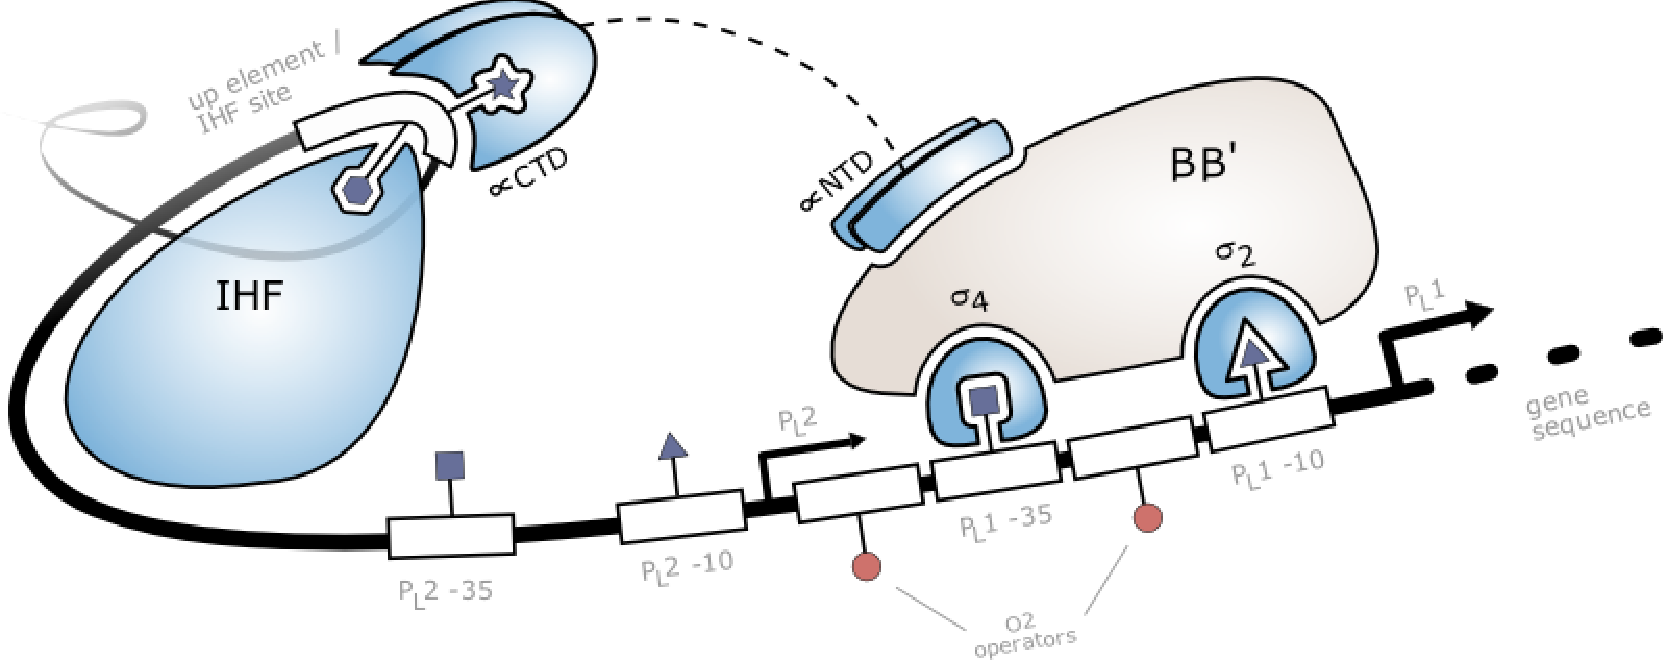
\includegraphics[width=\textwidth]{figures/fig1}
\caption[Short figure name.]{This is a figure that floats inline and here is its caption.
\label{fig:myInlineFigure}}
\end{figure}


Quisque facilisis erat a dui. Nam malesuada ornare dolor. Cras gravida, diam sit amet rhoncus ornare, erat elit consectetuer erat, id egestas pede nibh eget odio. Proin tincidunt, velit vel porta elementum, magna diam molestie sapien, non aliquet massa pede eu diam. Aliquam iaculis. Fusce et ipsum et nulla tristique facilisis. Donec eget sem sit amet ligula viverra gravida. Etiam vehicula urna vel turpis. Suspendisse sagittis ante a urna. Morbi a est quis orci consequat rutrum. Nullam egestas feugiat felis. Integer adipiscing semper ligula. Nunc molestie, nisl sit amet cursus convallis, sapien lectus pretium metus, vitae pretium enim wisi id lectus. Donec vestibulum. Etiam vel nibh. Nulla facilisi. Mauris pharetra. Donec augue. Fusce ultrices, neque id dignissim ultrices, tellus mauris dictum elit, vel lacinia enim metus eu nunc.

Proin at eros non eros adipiscing mollis. Donec semper turpis sed diam. Sed consequat ligula nec tortor. Integer eget sem. Ut vitae enim eu est vehicula gravida. Morbi ipsum ipsum, porta nec, tempor id, auctor vitae, purus. Pellentesque neque. Nulla luctus erat vitae libero. Integer nec enim. Phasellus aliquam enim et tortor. Quisque aliquet, quam elementum condimentum feugiat, tellus odio consectetuer wisi, vel nonummy sem neque in elit. Curabitur eleifend wisi iaculis ipsum. Pellentesque habitant morbi tristique senectus et netus et malesuada fames ac turpis egestas. In non velit non ligula laoreet ultrices. Praesent ultricies facilisis nisl. Vivamus luctus elit sit amet mi. Phasellus pellentesque, erat eget elementum volutpat, dolor nisl porta neque, vitae sodales ipsum nibh in ligula. Maecenas mattis pulvinar diam. Curabitur sed leo.

Nulla facilisi. In vel sem. Morbi id urna in diam dignissim feugiat. Proin molestie tortor eu velit. Aliquam erat volutpat. Nullam ultrices, diam tempus vulputate egestas, eros pede varius leo, sed imperdiet lectus est ornare odio. Lorem ipsum dolor sit amet, consectetuer adipiscing elit. Proin consectetuer velit in dui. Phasellus wisi purus, interdum vitae, rutrum accumsan, viverra in, velit. Sed enim risus, congue non, tristique in, commodo eu, metus. Aenean tortor mi, imperdiet id, gravida eu, posuere eu, felis. Mauris sollicitudin, turpis in hendrerit sodales, lectus ipsum pellentesque ligula, sit amet scelerisque urna nibh ut arcu. Aliquam in lacus. Vestibulum ante ipsum primis in faucibus orci luctus et ultrices posuere cubilia Curae; Nulla placerat aliquam wisi. Mauris viverra odio. Quisque fermentum pulvinar odio. Proin posuere est vitae ligula. Etiam euismod. Cras a eros.

Nunc auctor bibendum eros. Maecenas porta accumsan mauris. Etiam enim enim, elementum sed, bibendum quis, rhoncus non, metus. Fusce neque dolor, adipiscing sed, consectetuer et, lacinia sit amet, quam. Suspendisse wisi quam, consectetuer in, blandit sed, suscipit eu, eros. Etiam ligula enim, tempor ut, blandit nec, mollis eu, lectus. Nam cursus. Vivamus iaculis. Aenean risus purus, pharetra in, blandit quis, gravida a, turpis. Donec nisl. Aenean eget mi. Fusce mattis est id diam. Phasellus faucibus interdum sapien. Duis quis nunc. Sed enim.

Pellentesque vel dui sed orci faucibus iaculis. Suspendisse dictum magna id purus tincidunt rutrum. Nulla congue. Vivamus sit amet lorem posuere dui vulputate ornare. Phasellus mattis sollicitudin ligula. Duis dignissim felis et urna. Integer adipiscing congue metus. Nam pede. Etiam non wisi. Sed accumsan dolor ac augue. Pellentesque eget lectus. Aliquam nec dolor nec tellus ornare venenatis. Nullam blandit placerat sem. Curabitur quis ipsum. Mauris nisl tellus, aliquet eu, suscipit eu, ullamcorper quis, magna. Mauris elementum, pede at sodales vestibulum, nulla tortor congue massa, quis pellentesque odio dui id est. Cras faucibus augue.

%% Requires fltpage2 package
%%
% \begin{FPfigure}
% 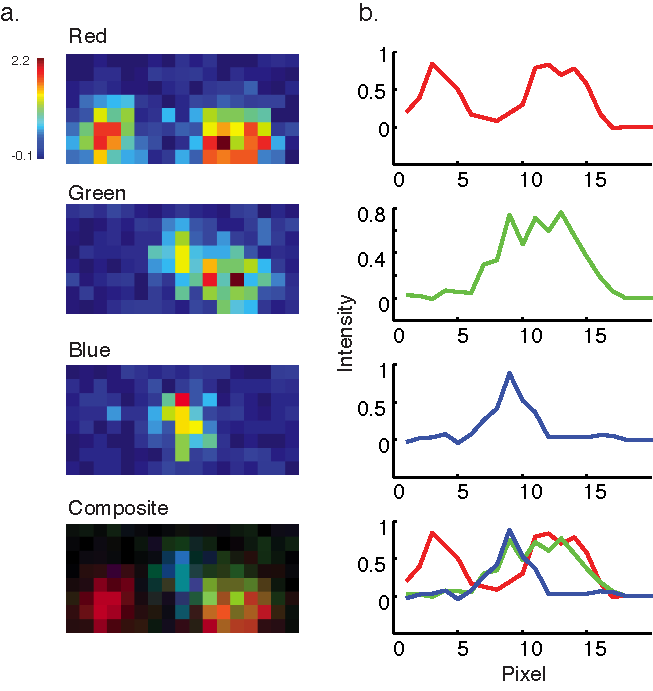
\includegraphics[width=\textwidth]{figures/fullpage}
% \caption[Short figure name.]{This is a full page figure using the FPfigure command. It takes up the whole page and the caption appears on the preceding page. Its useful for large figures. Harvard's rules about full page figures are tricky, but you don't have to worry about it because we took care of it for you. For example, the full figure is supposed to have a title in the same style as the caption but without the actual caption. The caption is supposed to appear alone on the preceding page with no other text. You do't have to worry about any of that. We have modified the fltpage package to make it work. This is a lengthy caption and it clearly would not fit on the same page as the figure. Note that you should only use the FPfigure command in instances where the figure really is too large. If the figure is small enough to fit by the caption than it does not produce the desired effect. Good luck with your thesis. I have to keep writing this to make the caption really long. LaTex is a lot of fun. You will enjoy working with it. Good luck on your post doctoral life! I am looking forward to mine. \label{fig:myFullPageFigure}}
% \end{FPfigure}
% \afterpage{\clearpage}

Suspendisse vestibulum dignissim quam. Integer vel augue. Phasellus nulla purus, interdum ac, venenatis non, varius rutrum, leo. Pellentesque habitant morbi tristique senectus et netus et malesuada fames ac turpis egestas. Duis a eros. Class aptent taciti sociosqu ad litora torquent per conubia nostra, per inceptos hymenaeos. Fusce magna mi, porttitor quis, convallis eget, sodales ac, urna. Phasellus luctus venenatis magna. Vivamus eget lacus. Nunc tincidunt convallis tortor. Duis eros mi, dictum vel, fringilla sit amet, fermentum id, sem. Phasellus nunc enim, faucibus ut, laoreet in, consequat id, metus. Vivamus dignissim. Cras lobortis tempor velit. Phasellus nec diam ac nisl lacinia tristique. Nullam nec metus id mi dictum dignissim. Nullam quis wisi non sem lobortis condimentum. Phasellus pulvinar, nulla non aliquam eleifend, tortor wisi scelerisque felis, in sollicitudin arcu ante lacinia leo.

Pellentesque habitant morbi tristique senectus et netus et malesuada fames ac turpis egestas. Vestibulum tortor quam, feugiat vitae, ultricies eget, tempor sit amet, ante. Donec eu libero sit amet quam egestas semper. Aenean ultricies mi vitae est. Mauris placerat eleifend leo. Quisque sit amet est et sapien ullamcorper pharetra. Vestibulum erat wisi, condimentum sed, commodo vitae, ornare sit amet, wisi. Aenean fermentum, elit eget tincidunt condimentum, eros ipsum rutrum orci, sagittis tempus lacus enim ac dui. Donec non enim in turpis pulvinar facilisis. Ut felis.

Cras sed ante. Phasellus in massa. Curabitur dolor eros, gravida et, hendrerit ac, cursus non, massa. Aliquam lorem. In hac habitasse platea dictumst. Cras eu mauris. Quisque lacus. Donec ipsum. Nullam vitae sem at nunc pharetra ultricies. Vivamus elit eros, ullamcorper a, adipiscing sit amet, porttitor ut, nibh. Maecenas adipiscing mollis massa. Nunc ut dui eget nulla venenatis aliquet. Sed luctus posuere justo. Cras vehicula varius turpis. Vivamus eros metus, tristique sit amet, molestie dignissim, malesuada et, urna.

Proin at eros non eros adipiscing mollis. Donec semper turpis sed diam. Sed consequat ligula nec tortor. Integer eget sem. Ut vitae enim eu est vehicula gravida. Morbi ipsum ipsum, porta nec, tempor id, auctor vitae, purus. Pellentesque neque. Nulla luctus erat vitae libero. Integer nec enim. Phasellus aliquam enim et tortor. Quisque aliquet, quam elementum condimentum feugiat, tellus odio consectetuer wisi, vel nonummy sem neque in elit. Curabitur eleifend wisi iaculis ipsum. Pellentesque habitant morbi tristique senectus et netus et malesuada fames ac turpis egestas. In non velit non ligula laoreet ultrices. Praesent ultricies facilisis nisl. Vivamus luctus elit sit amet mi. Phasellus pellentesque, erat eget elementum volutpat, dolor nisl porta neque, vitae sodales ipsum nibh in ligula. Maecenas mattis pulvinar diam. Curabitur sed leo.

Nulla facilisi. In vel sem. Morbi id urna in diam dignissim feugiat. Proin molestie tortor eu velit. Aliquam erat volutpat. Nullam ultrices, diam tempus vulputate egestas, eros pede varius leo, sed imperdiet lectus est ornare odio. Lorem ipsum dolor sit amet, consectetuer adipiscing elit. Proin consectetuer velit in dui. Phasellus wisi purus, interdum vitae, rutrum accumsan, viverra in, velit. Sed enim risus, congue non, tristique in, commodo eu, metus. Aenean tortor mi, imperdiet id, gravida eu, posuere eu, felis. Mauris sollicitudin, turpis in hendrerit sodales, lectus ipsum pellentesque ligula, sit amet scelerisque urna nibh ut arcu. Aliquam in lacus. Vestibulum ante ipsum primis in faucibus orci luctus et ultrices posuere cubilia Curae; Nulla placerat aliquam wisi. Mauris viverra odio. Quisque fermentum pulvinar odio. Proin posuere est vitae ligula. Etiam euismod. Cras a eros.

Nunc auctor bibendum eros. Maecenas porta accumsan mauris. Etiam enim enim, elementum sed, bibendum quis, rhoncus non, metus. Fusce neque dolor, adipiscing sed, consectetuer et, lacinia sit amet, quam. Suspendisse wisi quam, consectetuer in, blandit sed, suscipit eu, eros. Etiam ligula enim, tempor ut, blandit nec, mollis eu, lectus. Nam cursus. Vivamus iaculis. Aenean risus purus, pharetra in, blandit quis, gravida a, turpis. Donec nisl. Aenean eget mi. Fusce mattis est id diam. Phasellus faucibus interdum sapien. Duis quis nunc. Sed enim.

Pellentesque vel dui sed orci faucibus iaculis. Suspendisse dictum magna id purus tincidunt rutrum. Nulla congue. Vivamus sit amet lorem posuere dui vulputate ornare. Phasellus mattis sollicitudin ligula. Duis dignissim felis et urna. Integer adipiscing congue metus. Nam pede. Etiam non wisi. Sed accumsan dolor ac augue. Pellentesque eget lectus. Aliquam nec dolor nec tellus ornare venenatis. Nullam blandit placerat sem. Curabitur quis ipsum. Mauris nisl tellus, aliquet eu, suscipit eu, ullamcorper quis, magna. Mauris elementum, pede at sodales vestibulum, nulla tortor congue massa, quis pellentesque odio dui id est. Cras faucibus augue.

Suspendisse vestibulum dignissim quam. Integer vel augue. Phasellus nulla purus, interdum ac, venenatis non, varius rutrum, leo. Pellentesque habitant morbi tristique senectus et netus et malesuada fames ac turpis egestas. Duis a eros. Class aptent taciti sociosqu ad litora torquent per conubia nostra, per inceptos hymenaeos. Fusce magna mi, porttitor quis, convallis eget, sodales ac, urna. Phasellus luctus venenatis magna. Vivamus eget lacus. Nunc tincidunt convallis tortor. Duis eros mi, dictum vel, fringilla sit amet, fermentum id, sem. Phasellus nunc enim, faucibus ut, laoreet in, consequat id, metus. Vivamus dignissim. Cras lobortis tempor velit. Phasellus nec diam ac nisl lacinia tristique. Nullam nec metus id mi dictum dignissim. Nullam quis wisi non sem lobortis condimentum. Phasellus pulvinar, nulla non aliquam eleifend, tortor wisi scelerisque felis, in sollicitudin arcu ante lacinia leo.

Pellentesque habitant morbi tristique senectus et netus et malesuada fames ac turpis egestas. Vestibulum tortor quam, feugiat vitae, ultricies eget, tempor sit amet, ante. Donec eu libero sit amet quam egestas semper. Aenean ultricies mi vitae est. Mauris placerat eleifend leo. Quisque sit amet est et sapien ullamcorper pharetra. Vestibulum erat wisi, condimentum sed, commodo vitae, ornare sit amet, wisi. Aenean fermentum, elit eget tincidunt condimentum, eros ipsum rutrum orci, sagittis tempus lacus enim ac dui. Donec non enim in turpis pulvinar facilisis. Ut felis.

Cras sed ante. Phasellus in massa. Curabitur dolor eros, gravida et, hendrerit ac, cursus non, massa. Aliquam lorem. In hac habitasse platea dictumst. Cras eu mauris. Quisque lacus. Donec ipsum. Nullam vitae sem at nunc pharetra ultricies. Vivamus elit eros, ullamcorper a, adipiscing sit amet, porttitor ut, nibh. Maecenas adipiscing mollis massa. Nunc ut dui eget nulla venenatis aliquet. Sed luctus posuere justo. Cras vehicula varius turpis. Vivamus eros metus, tristique sit amet, molestie dignissim, malesuada et, urna.

Cras dictum. Maecenas ut turpis. In vitae erat ac orci dignissim eleifend. Nunc quis justo. Sed vel ipsum in purus tincidunt pharetra. Sed pulvinar, felis id consectetuer malesuada, enim nisl mattis elit, a facilisis tortor nibh quis leo. Sed augue lacus, pretium vitae, molestie eget, rhoncus quis, elit. Donec in augue. Fusce orci wisi, ornare id, mollis vel, lacinia vel, massa.

Lorem ipsum dolor sit amet, consectetuer adipiscing elit. Morbi commodo, ipsum sed pharetra gravida, orci magna rhoncus neque, id pulvinar odio lorem non turpis. Nullam sit amet enim. Suspendisse id velit vitae ligula volutpat condimentum. Aliquam erat volutpat. Sed quis velit. Nulla facilisi. Nulla libero. Vivamus pharetra posuere sapien. Nam consectetuer. Sed aliquam, nunc eget euismod ullamcorper, lectus nunc ullamcorper orci, fermentum bibendum enim nibh eget ipsum. Donec porttitor ligula eu dolor. Maecenas vitae nulla consequat libero cursus venenatis. Nam magna enim, accumsan eu, blandit sed, blandit a, eros.

Quisque facilisis erat a dui. Nam malesuada ornare dolor. Cras gravida, diam sit amet rhoncus ornare, erat elit consectetuer erat, id egestas pede nibh eget odio. Proin tincidunt, velit vel porta elementum, magna diam molestie sapien, non aliquet massa pede eu diam. Aliquam iaculis. Fusce et ipsum et nulla tristique facilisis. Donec eget sem sit amet ligula viverra gravida. Etiam vehicula urna vel turpis. Suspendisse sagittis ante a urna. Morbi a est quis orci consequat rutrum. Nullam egestas feugiat felis. Integer adipiscing semper ligula. Nunc molestie, nisl sit amet cursus convallis, sapien lectus pretium metus, vitae pretium enim wisi id lectus. Donec vestibulum. Etiam vel nibh. Nulla facilisi. Mauris pharetra. Donec augue. Fusce ultrices, neque id dignissim ultrices, tellus mauris dictum elit, vel lacinia enim metus eu nunc.

Proin at eros non eros adipiscing mollis. Donec semper turpis sed diam. Sed consequat ligula nec tortor. Integer eget sem. Ut vitae enim eu est vehicula gravida. Morbi ipsum ipsum, porta nec, tempor id, auctor vitae, purus. Pellentesque neque. Nulla luctus erat vitae libero. Integer nec enim. Phasellus aliquam enim et tortor. Quisque aliquet, quam elementum condimentum feugiat, tellus odio consectetuer wisi, vel nonummy sem neque in elit. Curabitur eleifend wisi iaculis ipsum. Pellentesque habitant morbi tristique senectus et netus et malesuada fames ac turpis egestas. In non velit non ligula laoreet ultrices. Praesent ultricies facilisis nisl. Vivamus luctus elit sit amet mi. Phasellus pellentesque, erat eget elementum volutpat, dolor nisl porta neque, vitae sodales ipsum nibh in ligula. Maecenas mattis pulvinar diam. Curabitur sed leo.

Nulla facilisi. In vel sem. Morbi id urna in diam dignissim feugiat. Proin molestie tortor eu velit. Aliquam erat volutpat. Nullam ultrices, diam tempus vulputate egestas, eros pede varius leo, sed imperdiet lectus est ornare odio. Lorem ipsum dolor sit amet, consectetuer adipiscing elit. Proin consectetuer velit in dui. Phasellus wisi purus, interdum vitae, rutrum accumsan, viverra in, velit. Sed enim risus, congue non, tristique in, commodo eu, metus. Aenean tortor mi, imperdiet id, gravida eu, posuere eu, felis. Mauris sollicitudin, turpis in hendrerit sodales, lectus ipsum pellentesque ligula, sit amet scelerisque urna nibh ut arcu. Aliquam in lacus. Vestibulum ante ipsum primis in faucibus orci luctus et ultrices posuere cubilia Curae; Nulla placerat aliquam wisi. Mauris viverra odio. Quisque fermentum pulvinar odio. Proin posuere est vitae ligula. Etiam euismod. Cras a eros.

Nunc auctor bibendum eros. Maecenas porta accumsan mauris. Etiam enim enim, elementum sed, bibendum quis, rhoncus non, metus. Fusce neque dolor, adipiscing sed, consectetuer et, lacinia sit amet, quam. Suspendisse wisi quam, consectetuer in, blandit sed, suscipit eu, eros. Etiam ligula enim, tempor ut, blandit nec, mollis eu, lectus. Nam cursus. Vivamus iaculis. Aenean risus purus, pharetra in, blandit quis, gravida a, turpis. Donec nisl. Aenean eget mi. Fusce mattis est id diam. Phasellus faucibus interdum sapien. Duis quis nunc. Sed enim.

Pellentesque vel dui sed orci faucibus iaculis. Suspendisse dictum magna id purus tincidunt rutrum. Nulla congue. Vivamus sit amet lorem posuere dui vulputate ornare. Phasellus mattis sollicitudin ligula. Duis dignissim felis et urna. Integer adipiscing congue metus. Nam pede. Etiam non wisi. Sed accumsan dolor ac augue. Pellentesque eget lectus. Aliquam nec dolor nec tellus ornare venenatis. Nullam blandit placerat sem. Curabitur quis ipsum. Mauris nisl tellus, aliquet eu, suscipit eu, ullamcorper quis, magna. Mauris elementum, pede at sodales vestibulum, nulla tortor congue massa, quis pellentesque odio dui id est. Cras faucibus augue.

Suspendisse vestibulum dignissim quam. Integer vel augue. Phasellus nulla purus, interdum ac, venenatis non, varius rutrum, leo. Pellentesque habitant morbi tristique senectus et netus et malesuada fames ac turpis egestas. Duis a eros. Class aptent taciti sociosqu ad litora torquent per conubia nostra, per inceptos hymenaeos. Fusce magna mi, porttitor quis, convallis eget, sodales ac, urna. Phasellus luctus venenatis magna. Vivamus eget lacus. Nunc tincidunt convallis tortor. Duis eros mi, dictum vel, fringilla sit amet, fermentum id, sem. Phasellus nunc enim, faucibus ut, laoreet in, consequat id, metus. Vivamus dignissim. Cras lobortis tempor velit. Phasellus nec diam ac nisl lacinia tristique. Nullam nec metus id mi dictum dignissim. Nullam quis wisi non sem lobortis condimentum. Phasellus pulvinar, nulla non aliquam eleifend, tortor wisi scelerisque felis, in sollicitudin arcu ante lacinia leo.

Pellentesque habitant morbi tristique senectus et netus et malesuada fames ac turpis egestas. Vestibulum tortor quam, feugiat vitae, ultricies eget, tempor sit amet, ante. Donec eu libero sit amet quam egestas semper. Aenean ultricies mi vitae est. Mauris placerat eleifend leo. Quisque sit amet est et sapien ullamcorper pharetra. Vestibulum erat wisi, condimentum sed, commodo vitae, ornare sit amet, wisi. Aenean fermentum, elit eget tincidunt condimentum, eros ipsum rutrum orci, sagittis tempus lacus enim ac dui. Donec non enim in turpis pulvinar facilisis. Ut felis.

Cras sed ante. Phasellus in massa. Curabitur dolor eros, gravida et, hendrerit ac, cursus non, massa. Aliquam lorem. In hac habitasse platea dictumst. Cras eu mauris. Quisque lacus. Donec ipsum. Nullam vitae sem at nunc pharetra ultricies. Vivamus elit eros, ullamcorper a, adipiscing sit amet, porttitor ut, nibh. Maecenas adipiscing mollis massa. Nunc ut dui eget nulla venenatis aliquet. Sed luctus posuere justo. Cras vehicula varius turpis. Vivamus eros metus, tristique sit amet, molestie dignissim, malesuada et, urna.

Cras dictum. Maecenas ut turpis. In vitae erat ac orci dignissim eleifend. Nunc quis justo. Sed vel ipsum in purus tincidunt pharetra. Sed pulvinar, felis id consectetuer malesuada, enim nisl mattis elit, a facilisis tortor nibh quis leo. Sed augue lacus, pretium vitae, molestie eget, rhoncus quis, elit. Donec in augue. Fusce orci wisi, ornare id, mollis vel, lacinia vel, massa.

Lorem ipsum dolor sit amet, consectetuer adipiscing elit. Morbi commodo, ipsum sed pharetra gravida, orci magna rhoncus neque, id pulvinar odio lorem non turpis. Nullam sit amet enim. Suspendisse id velit vitae ligula volutpat condimentum. Aliquam erat volutpat. Sed quis velit. Nulla facilisi. Nulla libero. Vivamus pharetra posuere sapien. Nam consectetuer. Sed aliquam, nunc eget euismod ullamcorper, lectus nunc ullamcorper orci, fermentum bibendum enim nibh eget ipsum. Donec porttitor ligula eu dolor. Maecenas vitae nulla consequat libero cursus venenatis. Nam magna enim, accumsan eu, blandit sed, blandit a, eros.

Quisque facilisis erat a dui. Nam malesuada ornare dolor. Cras gravida, diam sit amet rhoncus ornare, erat elit consectetuer erat, id egestas pede nibh eget odio. Proin tincidunt, velit vel porta elementum, magna diam molestie sapien, non aliquet massa pede eu diam. Aliquam iaculis. Fusce et ipsum et nulla tristique facilisis. Donec eget sem sit amet ligula viverra gravida. Etiam vehicula urna vel turpis. Suspendisse sagittis ante a urna. Morbi a est quis orci consequat rutrum. Nullam egestas feugiat felis. Integer adipiscing semper ligula. Nunc molestie, nisl sit amet cursus convallis, sapien lectus pretium metus, vitae pretium enim wisi id lectus. Donec vestibulum. Etiam vel nibh. Nulla facilisi. Mauris pharetra. Donec augue. Fusce ultrices, neque id dignissim ultrices, tellus mauris dictum elit, vel lacinia enim metus eu nunc.

Proin at eros non eros adipiscing mollis. Donec semper turpis sed diam. Sed consequat ligula nec tortor. Integer eget sem. Ut vitae enim eu est vehicula gravida. Morbi ipsum ipsum, porta nec, tempor id, auctor vitae, purus. Pellentesque neque. Nulla luctus erat vitae libero. Integer nec enim. Phasellus aliquam enim et tortor. Quisque aliquet, quam elementum condimentum feugiat, tellus odio consectetuer wisi, vel nonummy sem neque in elit. Curabitur eleifend wisi iaculis ipsum. Pellentesque habitant morbi tristique senectus et netus et malesuada fames ac turpis egestas. In non velit non ligula laoreet ultrices. Praesent ultricies facilisis nisl. Vivamus luctus elit sit amet mi. Phasellus pellentesque, erat eget elementum volutpat, dolor nisl porta neque, vitae sodales ipsum nibh in ligula. Maecenas mattis pulvinar diam. Curabitur sed leo.

Nulla facilisi. In vel sem. Morbi id urna in diam dignissim feugiat. Proin molestie tortor eu velit. Aliquam erat volutpat. Nullam ultrices, diam tempus vulputate egestas, eros pede varius leo, sed imperdiet lectus est ornare odio. Lorem ipsum dolor sit amet, consectetuer adipiscing elit. Proin consectetuer velit in dui. Phasellus wisi purus, interdum vitae, rutrum accumsan, viverra in, velit. Sed enim risus, congue non, tristique in, commodo eu, metus. Aenean tortor mi, imperdiet id, gravida eu, posuere eu, felis. Mauris sollicitudin, turpis in hendrerit sodales, lectus ipsum pellentesque ligula, sit amet scelerisque urna nibh ut arcu. Aliquam in lacus. Vestibulum ante ipsum primis in faucibus orci luctus et ultrices posuere cubilia Curae; Nulla placerat aliquam wisi. Mauris viverra odio. Quisque fermentum pulvinar odio. Proin posuere est vitae ligula. Etiam euismod. Cras a eros.

Nunc auctor bibendum eros. Maecenas porta accumsan mauris. Etiam enim enim, elementum sed, bibendum quis, rhoncus non, metus. Fusce neque dolor, adipiscing sed, consectetuer et, lacinia sit amet, quam. Suspendisse wisi quam, consectetuer in, blandit sed, suscipit eu, eros. Etiam ligula enim, tempor ut, blandit nec, mollis eu, lectus. Nam cursus. Vivamus iaculis. Aenean risus purus, pharetra in, blandit quis, gravida a, turpis. Donec nisl. Aenean eget mi. Fusce mattis est id diam. Phasellus faucibus interdum sapien. Duis quis nunc. Sed enim.


Cras sed ante. Phasellus in massa. Curabitur dolor eros, gravida et, hendrerit ac, cursus non, massa. Aliquam lorem. In hac habitasse platea dictumst. Cras eu mauris. Quisque lacus. Donec ipsum. Nullam vitae sem at nunc pharetra ultricies. Vivamus elit eros, ullamcorper a, adipiscing sit amet, porttitor ut, nibh. Maecenas adipiscing mollis massa. Nunc ut dui eget nulla venenatis aliquet. Sed luctus posuere justo. Cras vehicula varius turpis. Vivamus eros metus, tristique sit amet, molestie dignissim, malesuada et, urna.

Cras dictum. Maecenas ut turpis. In vitae erat ac orci dignissim eleifend. Nunc quis justo. Sed vel ipsum in purus tincidunt pharetra. Sed pulvinar, felis id consectetuer malesuada, enim nisl mattis elit, a facilisis tortor nibh quis leo. Sed augue lacus, pretium vitae, molestie eget, rhoncus quis, elit. Donec in augue. Fusce orci wisi, ornare id, mollis vel, lacinia vel, massa.

Lorem ipsum dolor sit amet, consectetuer adipiscing elit. Morbi commodo, ipsum sed pharetra gravida, orci magna rhoncus neque, id pulvinar odio lorem non turpis. Nullam sit amet enim. Suspendisse id velit vitae ligula volutpat condimentum. Aliquam erat volutpat. Sed quis velit. Nulla facilisi. Nulla libero. Vivamus pharetra posuere sapien. Nam consectetuer. Sed aliquam, nunc eget euismod ullamcorper, lectus nunc ullamcorper orci, fermentum bibendum enim nibh eget ipsum. Donec porttitor ligula eu dolor. Maecenas vitae nulla consequat libero cursus venenatis. Nam magna enim, accumsan eu, blandit sed, blandit a, eros.

Quisque facilisis erat a dui. Nam malesuada ornare dolor. Cras gravida, diam sit amet rhoncus ornare, erat elit consectetuer erat, id egestas pede nibh eget odio. Proin tincidunt, velit vel porta elementum, magna diam molestie sapien, non aliquet massa pede eu diam. Aliquam iaculis. Fusce et ipsum et nulla tristique facilisis. Donec eget sem sit amet ligula viverra gravida. Etiam vehicula urna vel turpis. Suspendisse sagittis ante a urna. Morbi a est quis orci consequat rutrum. Nullam egestas feugiat felis. Integer adipiscing semper ligula. Nunc molestie, nisl sit amet cursus convallis, sapien lectus pretium metus, vitae pretium enim wisi id lectus. Donec vestibulum. Etiam vel nibh. Nulla facilisi. Mauris pharetra. Donec augue. Fusce ultrices, neque id dignissim ultrices, tellus mauris dictum elit, vel lacinia enim metus eu nunc.

Proin at eros non eros adipiscing mollis. Donec semper turpis sed diam. Sed consequat ligula nec tortor. Integer eget sem. Ut vitae enim eu est vehicula gravida. Morbi ipsum ipsum, porta nec, tempor id, auctor vitae, purus. Pellentesque neque. Nulla luctus erat vitae libero. Integer nec enim. Phasellus aliquam enim et tortor. Quisque aliquet, quam elementum condimentum feugiat, tellus odio consectetuer wisi, vel nonummy sem neque in elit. Curabitur eleifend wisi iaculis ipsum. Pellentesque habitant morbi tristique senectus et netus et malesuada fames ac turpis egestas. In non velit non ligula laoreet ultrices. Praesent ultricies facilisis nisl. Vivamus luctus elit sit amet mi. Phasellus pellentesque, erat eget elementum volutpat, dolor nisl porta neque, vitae sodales ipsum nibh in ligula. Maecenas mattis pulvinar diam. Curabitur sed leo.

Nulla facilisi. In vel sem. Morbi id urna in diam dignissim feugiat. Proin molestie tortor eu velit. Aliquam erat volutpat. Nullam ultrices, diam tempus vulputate egestas, eros pede varius leo, sed imperdiet lectus est ornare odio. Lorem ipsum dolor sit amet, consectetuer adipiscing elit. Proin consectetuer velit in dui. Phasellus wisi purus, interdum vitae, rutrum accumsan, viverra in, velit. Sed enim risus, congue non, tristique in, commodo eu, metus. Aenean tortor mi, imperdiet id, gravida eu, posuere eu, felis. Mauris sollicitudin, turpis in hendrerit sodales, lectus ipsum pellentesque ligula, sit amet scelerisque urna nibh ut arcu. Aliquam in lacus. Vestibulum ante ipsum primis in faucibus orci luctus et ultrices posuere cubilia Curae; Nulla placerat aliquam wisi. Mauris viverra odio. Quisque fermentum pulvinar odio. Proin posuere est vitae ligula. Etiam euismod. Cras a eros.

Nunc auctor bibendum eros. Maecenas porta accumsan mauris. Etiam enim enim, elementum sed, bibendum quis, rhoncus non, metus. Fusce neque dolor, adipiscing sed, consectetuer et, lacinia sit amet, quam. Suspendisse wisi quam, consectetuer in, blandit sed, suscipit eu, eros. Etiam ligula enim, tempor ut, blandit nec, mollis eu, lectus. Nam cursus. Vivamus iaculis. Aenean risus purus, pharetra in, blandit quis, gravida a, turpis. Donec nisl. Aenean eget mi. Fusce mattis est id diam. Phasellus faucibus interdum sapien. Duis quis nunc. Sed enim.

Pellentesque vel dui sed orci faucibus iaculis. Suspendisse dictum magna id purus tincidunt rutrum. Nulla congue. Vivamus sit amet lorem posuere dui vulputate ornare. Phasellus mattis sollicitudin ligula. Duis dignissim felis et urna. Integer adipiscing congue metus. Nam pede. Etiam non wisi. Sed accumsan dolor ac augue. Pellentesque eget lectus. Aliquam nec dolor nec tellus ornare venenatis. Nullam blandit placerat sem. Curabitur quis ipsum. Mauris nisl tellus, aliquet eu, suscipit eu, ullamcorper quis, magna. Mauris elementum, pede at sodales vestibulum, nulla tortor congue massa, quis pellentesque odio dui id est. Cras faucibus augue.

Suspendisse vestibulum dignissim quam. Integer vel augue. Phasellus nulla purus, interdum ac, venenatis non, varius rutrum, leo. Pellentesque habitant morbi tristique senectus et netus et malesuada fames ac turpis egestas. Duis a eros. Class aptent taciti sociosqu ad litora torquent per conubia nostra, per inceptos hymenaeos. Fusce magna mi, porttitor quis, convallis eget, sodales ac, urna. Phasellus luctus venenatis magna. Vivamus eget lacus. Nunc tincidunt convallis tortor. Duis eros mi, dictum vel, fringilla sit amet, fermentum id, sem. Phasellus nunc enim, faucibus ut, laoreet in, consequat id, metus. Vivamus dignissim. Cras lobortis tempor velit. Phasellus nec diam ac nisl lacinia tristique. Nullam nec metus id mi dictum dignissim. Nullam quis wisi non sem lobortis condimentum. Phasellus pulvinar, nulla non aliquam eleifend, tortor wisi scelerisque felis, in sollicitudin arcu ante lacinia leo.

Pellentesque habitant morbi tristique senectus et netus et malesuada fames ac turpis egestas. Vestibulum tortor quam, feugiat vitae, ultricies eget, tempor sit amet, ante. Donec eu libero sit amet quam egestas semper. Aenean ultricies mi vitae est. Mauris placerat eleifend leo. Quisque sit amet est et sapien ullamcorper pharetra. Vestibulum erat wisi, condimentum sed, commodo vitae, ornare sit amet, wisi. Aenean fermentum, elit eget tincidunt condimentum, eros ipsum rutrum orci, sagittis tempus lacus enim ac dui. Donec non enim in turpis pulvinar facilisis. Ut felis.

Cras sed ante. Phasellus in massa. Curabitur dolor eros, gravida et, hendrerit ac, cursus non, massa. Aliquam lorem. In hac habitasse platea dictumst. Cras eu mauris. Quisque lacus. Donec ipsum. Nullam vitae sem at nunc pharetra ultricies. Vivamus elit eros, ullamcorper a, adipiscing sit amet, porttitor ut, nibh. Maecenas adipiscing mollis massa. Nunc ut dui eget nulla venenatis aliquet. Sed luctus posuere justo. Cras vehicula varius turpis. Vivamus eros metus, tristique sit amet, molestie dignissim, malesuada et, urna.

Cras dictum. Maecenas ut turpis. In vitae erat ac orci dignissim eleifend. Nunc quis justo. Sed vel ipsum in purus tincidunt pharetra. Sed pulvinar, felis id consectetuer malesuada, enim nisl mattis elit, a facilisis tortor nibh quis leo. Sed augue lacus, pretium vitae, molestie eget, rhoncus quis, elit. Donec in augue. Fusce orci wisi, ornare id, mollis vel, lacinia vel, massa.

Lorem ipsum dolor sit amet, consectetuer adipiscing elit. Morbi commodo, ipsum sed pharetra gravida, orci magna rhoncus neque, id pulvinar odio lorem non turpis. Nullam sit amet enim. Suspendisse id velit vitae ligula volutpat condimentum. Aliquam erat volutpat. Sed quis velit. Nulla facilisi. Nulla libero. Vivamus pharetra posuere sapien. Nam consectetuer. Sed aliquam, nunc eget euismod ullamcorper, lectus nunc ullamcorper orci, fermentum bibendum enim nibh eget ipsum. Donec porttitor ligula eu dolor. Maecenas vitae nulla consequat libero cursus venenatis. Nam magna enim, accumsan eu, blandit sed, blandit a, eros.

Quisque facilisis erat a dui. Nam malesuada ornare dolor. Cras gravida, diam sit amet rhoncus ornare, erat elit consectetuer erat, id egestas pede nibh eget odio. Proin tincidunt, velit vel porta elementum, magna diam molestie sapien, non aliquet massa pede eu diam. Aliquam iaculis. Fusce et ipsum et nulla tristique facilisis. Donec eget sem sit amet ligula viverra gravida. Etiam vehicula urna vel turpis. Suspendisse sagittis ante a urna. Morbi a est quis orci consequat rutrum. Nullam egestas feugiat felis. Integer adipiscing semper ligula. Nunc molestie, nisl sit amet cursus convallis, sapien lectus pretium metus, vitae pretium enim wisi id lectus. Donec vestibulum. Etiam vel nibh. Nulla facilisi. Mauris pharetra. Donec augue. Fusce ultrices, neque id dignissim ultrices, tellus mauris dictum elit, vel lacinia enim metus eu nunc.

Proin at eros non eros adipiscing mollis. Donec semper turpis sed diam. Sed consequat ligula nec tortor. Integer eget sem. Ut vitae enim eu est vehicula gravida. Morbi ipsum ipsum, porta nec, tempor id, auctor vitae, purus. Pellentesque neque. Nulla luctus erat vitae libero. Integer nec enim. Phasellus aliquam enim et tortor. Quisque aliquet, quam elementum condimentum feugiat, tellus odio consectetuer wisi, vel nonummy sem neque in elit. Curabitur eleifend wisi iaculis ipsum. Pellentesque habitant morbi tristique senectus et netus et malesuada fames ac turpis egestas. In non velit non ligula laoreet ultrices. Praesent ultricies facilisis nisl. Vivamus luctus elit sit amet mi. Phasellus pellentesque, erat eget elementum volutpat, dolor nisl porta neque, vitae sodales ipsum nibh in ligula. Maecenas mattis pulvinar diam. Curabitur sed leo.

Nulla facilisi. In vel sem. Morbi id urna in diam dignissim feugiat. Proin molestie tortor eu velit. Aliquam erat volutpat. Nullam ultrices, diam tempus vulputate egestas, eros pede varius leo, sed imperdiet lectus est ornare odio. Lorem ipsum dolor sit amet, consectetuer adipiscing elit. Proin consectetuer velit in dui. Phasellus wisi purus, interdum vitae, rutrum accumsan, viverra in, velit. Sed enim risus, congue non, tristique in, commodo eu, metus. Aenean tortor mi, imperdiet id, gravida eu, posuere eu, felis. Mauris sollicitudin, turpis in hendrerit sodales, lectus ipsum pellentesque ligula, sit amet scelerisque urna nibh ut arcu. Aliquam in lacus. Vestibulum ante ipsum primis in faucibus orci luctus et ultrices posuere cubilia Curae; Nulla placerat aliquam wisi. Mauris viverra odio. Quisque fermentum pulvinar odio. Proin posuere est vitae ligula. Etiam euismod. Cras a eros.

Nunc auctor bibendum eros. Maecenas porta accumsan mauris. Etiam enim enim, elementum sed, bibendum quis, rhoncus non, metus. Fusce neque dolor, adipiscing sed, consectetuer et, lacinia sit amet, quam. Suspendisse wisi quam, consectetuer in, blandit sed, suscipit eu, eros. Etiam ligula enim, tempor ut, blandit nec, mollis eu, lectus. Nam cursus. Vivamus iaculis. Aenean risus purus, pharetra in, blandit quis, gravida a, turpis. Donec nisl. Aenean eget mi. Fusce mattis est id diam. Phasellus faucibus interdum sapien. Duis quis nunc. Sed enim.

Pellentesque vel dui sed orci faucibus iaculis. Suspendisse dictum magna id purus tincidunt rutrum. Nulla congue. Vivamus sit amet lorem posuere dui vulputate ornare. Phasellus mattis sollicitudin ligula. Duis dignissim felis et urna. Integer adipiscing congue metus. Nam pede. Etiam non wisi. Sed accumsan dolor ac augue. Pellentesque eget lectus. Aliquam nec dolor nec tellus ornare venenatis. Nullam blandit placerat sem. Curabitur quis ipsum. Mauris nisl tellus, aliquet eu, suscipit eu, ullamcorper quis, magna. Mauris elementum, pede at sodales vestibulum, nulla tortor congue massa, quis pellentesque odio dui id est. Cras faucibus augue.

Suspendisse vestibulum dignissim quam. Integer vel augue. Phasellus nulla purus, interdum ac, venenatis non, varius rutrum, leo. Pellentesque habitant morbi tristique senectus et netus et malesuada fames ac turpis egestas. Duis a eros. Class aptent taciti sociosqu ad litora torquent per conubia nostra, per inceptos hymenaeos. Fusce magna mi, porttitor quis, convallis eget, sodales ac, urna. Phasellus luctus venenatis magna. Vivamus eget lacus. Nunc tincidunt convallis tortor. Duis eros mi, dictum vel, fringilla sit amet, fermentum id, sem. Phasellus nunc enim, faucibus ut, laoreet in, consequat id, metus. Vivamus dignissim. Cras lobortis tempor velit. Phasellus nec diam ac nisl lacinia tristique. Nullam nec metus id mi dictum dignissim. Nullam quis wisi non sem lobortis condimentum. Phasellus pulvinar, nulla non aliquam eleifend, tortor wisi scelerisque felis, in sollicitudin arcu ante lacinia leo.

%# -*- coding: utf-8-unix -*-
%%==================================================

\chapter{{\LaTeX} 排版例子}

\section{数学排版}

\subsection{公式排版}

这里有举一个长公式排版的例子,来自\href{http://www.tex.ac.uk/tex-archive/info/math/voss/mathmode/Mathmode.pdf}{《Math mode》}:

\begin{multline}
  \frac {1}{2}\Delta (f_{ij}f^{ij})=
  2\left (\sum _{i<j}\chi _{ij}(\sigma _{i}-
    \sigma _{j}) ^{2}+ f^{ij}\nabla _{j}\nabla _{i}(\Delta f)+\right .\\
  \left .+\nabla _{k}f_{ij}\nabla ^{k}f^{ij}+
    f^{ij}f^{k}\left [2\nabla _{i}R_{jk}-
      \nabla _{k}R_{ij}\right ]\vphantom {\sum _{i<j}}\right )
\end{multline}

下面演示了mathtools宏包中可伸长符号(箭头、等号的例子)的例子。
\begin{displaymath}
A \xleftarrow[n=0]{} B \xrightarrow[LongLongLongLong]{n>0} C 
\end{displaymath}

\begin{eqnarray}
f(x) & \xleftrightarrow[]{A=B}  & B \\
& \xleftharpoondown[below]{above} & B \nonumber \\
& \xLeftrightarrow[below]{above} & B
\end{eqnarray}

又如:
\begin{align}
\label{eq:none}
& I(X_3;X_4)-I(X_3;X_4\mid{}X_1)-I(X_3;X_4\mid{}X_2) \nonumber \\
= & [I(X_3;X_4)-I(X_3;X_4\mid{}X_1)]-I(X_3;X_4\mid{}\tilde{X}_2) \\
= & I(X_1;X_3;X_4)-I(X_3;X_4\mid{}\tilde{X}_2)
\end{align}

\subsection{国际单位制}

使用\verb+siunitx+宏包可以方便地输入国际标准单位制单位,例如\verb+\SI{5}{\um}+可以得到\SI{5}{\um}。

\subsection{定理环境}

模板中定义了丰富的定理环境
algo(算法),thm(定理),lem(引理),prop(命题),cor(推论),defn(定义),conj(猜想),exmp(例),rem(注),case(情形),
bthm(断言定理),blem(断言引理),bprop(断言命题),bcor(断言推论)。
amsmath还提供了一个proof(证明)的环境。
这里举一个“定理”和“证明”的例子。
\begin{thm}[留数定理]
\label{thm:res}
  假设$U$是复平面上的一个单连通开子集,$a_1,\ldots,a_n$是复平面上有限个点,$f$是定义在$U\backslash \{a_1,\ldots,a_n\}$上的全纯函数,
  如果$\gamma$是一条把$a_1,\ldots,a_n$包围起来的可求长曲线,但不经过任何一个$a_k$,并且其起点与终点重合,那么:

  \begin{equation}
    \label{eq:res}
    \ointop_{\gamma}f(z)\,\mathrm{d}z = 2\uppi\mathbf{i}\sum^n_{k=1}\mathrm{I}(\gamma,a_k)\mathrm{Res}(f,a_k)
  \end{equation}

  如果$\gamma$是若尔当曲线,那么$\mathrm{I}(\gamma, a_k)=1$,因此:

  \begin{equation}
    \label{eq:resthm}
    \ointop_{\gamma}f(z)\,\mathrm{d}z = 2\uppi\mathbf{i}\sum^n_{k=1}\mathrm{Res}(f,a_k)
  \end{equation}

      % \oint_\gamma f(z)\, dz = 2\pi i \sum_{k=1}^n \mathrm{Res}(f, a_k ). 

  在这里,$\mathrm{Res}(f, a_k)$表示$f$在点$a_k$的留数,$\mathrm{I}(\gamma,a_k)$表示$\gamma$关于点$a_k$的卷绕数。
  卷绕数是一个整数,它描述了曲线$\gamma$绕过点$a_k$的次数。如果$\gamma$依逆时针方向绕着$a_k$移动,卷绕数就是一个正数,
  如果$\gamma$根本不绕过$a_k$,卷绕数就是零。

  定理\ref{thm:res}的证明。
  
  \begin{proof}
    首先,由……

    其次,……

    所以……
  \end{proof}
\end{thm}

上面的公式例子中,有一些细节希望大家注意。微分号d应该使用“直立体”也就是用mathrm包围起来。
并且,微分号和被积函数之间应该有一段小间隔,可以插入\verb+\,+得到。
斜体的$d$通常只作为一般变量。
i,j作为虚数单位时,也应该使用“直立体”为了明显,还加上了粗体,例如\verb+\mathbf{i}+。斜体$i,j$通常用作表示“序号”。
其他字母在表示常量时,也推荐使用“直立体”譬如,圆周率$\uppi$(需要upgreek宏包),自然对数的底$\mathrm{e}$。
不过,我个人觉得斜体的$e$和$\pi$很潇洒,在不至于引起混淆的情况下,我也用这两个字母的斜体表示对应的常量。

\section{插入图像}

\subsection{支持的图片格式}

\XeTeX 可以很方便地插入PDF、PNG、JPG格式的图片。

JPG的例子如\ref{fig:csulogo}所示,PNG的例子如\ref{fig:tem}所示,
\begin{figure}[!htp]
  \centering
  
\includegraphics[scale=0.4]{example/csulogo.jpg}
  \caption{中南大学校徽}
  \label{fig:csulogo}
\end{figure}

\begin{figure}[!htp]
	\centering
	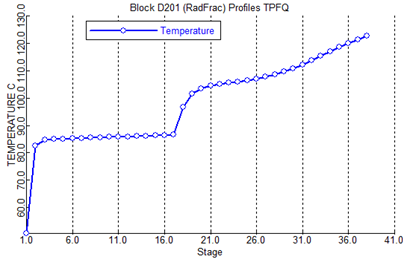
\includegraphics[scale=0.6]{example/tem.png}
	\caption{塔板温度分布图}
	\label{fig:tem}
\end{figure}

这里还有插入EPS图像和PDF图像的例子,如图\ref{fig:epspdf:a}和图\ref{fig:epspdf:b}。这里将EPS和PDF图片作为子图插入,每个子图有自己的小标题。子图标题使用subcaption宏包添加。

\begin{figure}[!htp]
  \centering
  \subcaptionbox{EPS 图像\label{fig:epspdf:a}}[3cm] %标题的长度,超过则会换行,如下一个小图。
    {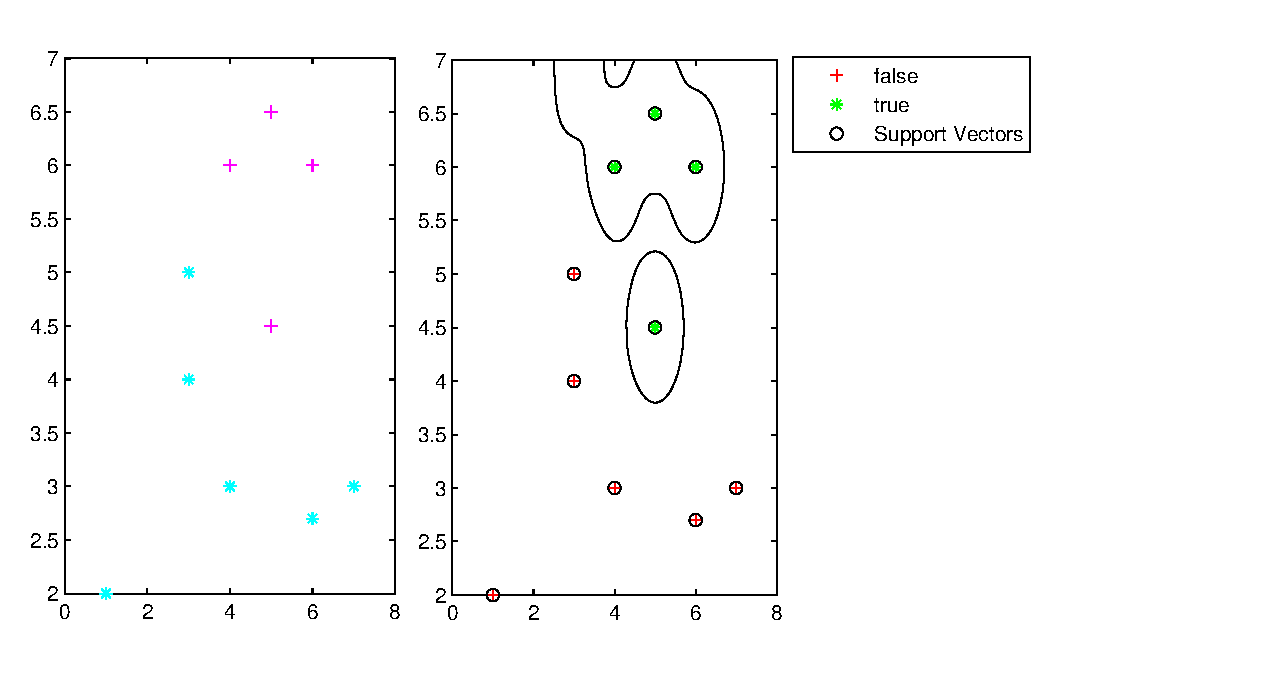
\includegraphics[height=4cm]{example/fig14.eps}}
  \hspace{4em}
  \subcaptionbox{PDF 图像。如果标题很长的话,它会自动换行\label{fig:epspdf:b}}
    {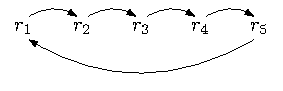
\includegraphics{example/permutation.pdf}}
  \caption{插入eps和pdf的例子(使用 subcaptionbox 方式)}
  \label{fig:pdfeps-subcaptionbox}
\end{figure}

\begin{figure}[!htp]
  \centering
  \begin{subfigure}{2.5cm}
    \centering
    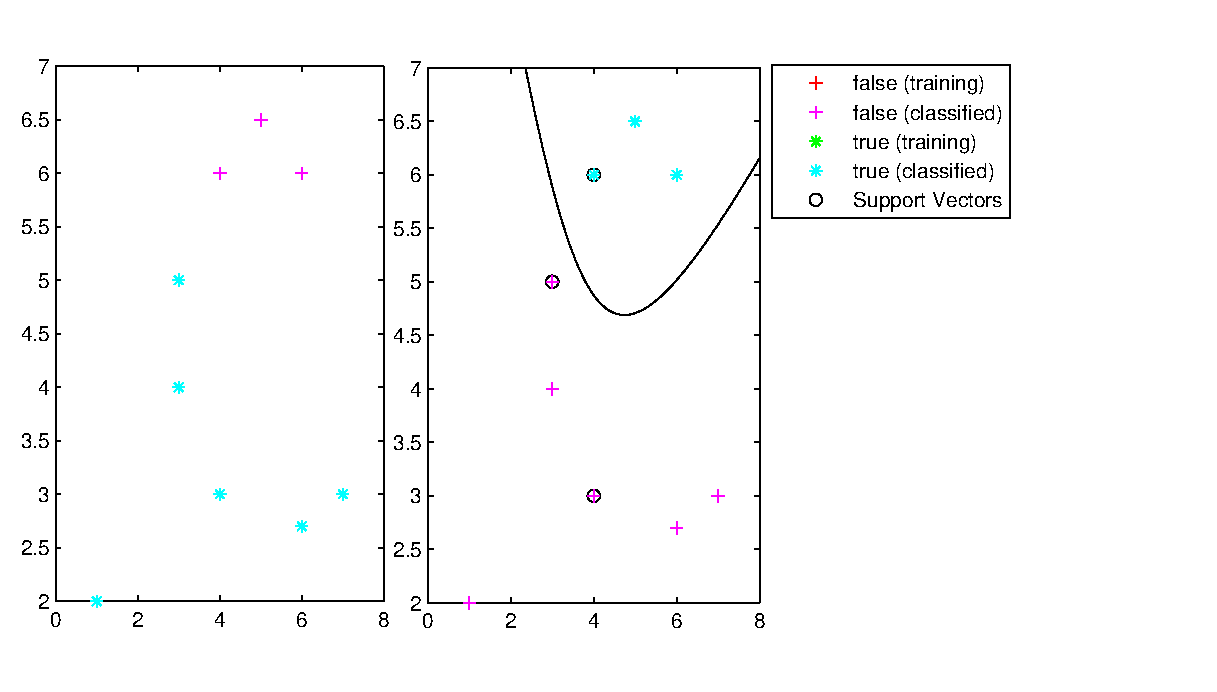
\includegraphics[height=3cm]{example/fig13.eps}
    \caption{EPS 图像}
  \end{subfigure}
  \hspace{4em}
  \begin{subfigure}{0.4\textwidth}
    \centering
    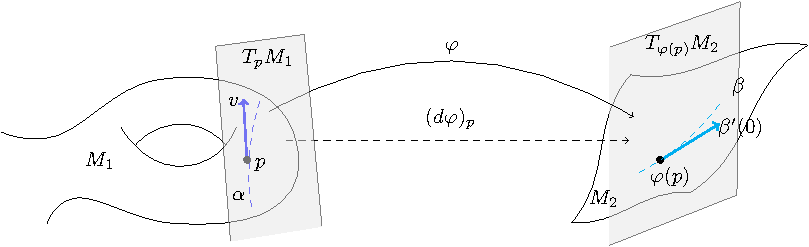
\includegraphics[height=2cm]{example/tangentmap.pdf}
    \caption{PDF 图像,注意这个图略矮些。subfigure中同一行的子图在顶端对齐。}
  \end{subfigure}
  \caption{插入eps和pdf的例子(使用 subfigure 方式)}
  \label{fig:pdfeps-subfigure}
\end{figure}

更多关于 \LaTeX 插图的例子可以参考\href{http://www.cs.duke.edu/junhu/Graphics3.pdf}{《\LaTeX 插图指南》}。

\subsection{绘制流程图}

图\ref{fig:flow_chart}是一张流程图示意。使用tikz环境,搭配四种预定义节点(\verb+startstop+、\verb+process+、\verb+decision+和\verb+io+),可以容易地绘制出流程图。
\begin{figure}[!htp]
    \centering
    \resizebox{6cm}{!}{\begin{tikzpicture}[node distance=2cm]
    \node (pic) [startstop] {待测图片};
    \node (bg) [io, below of=pic] {读取背景};
    \node (pair) [process, below of=bg] {匹配特征点对};
    \node (threshold) [decision, below of=pair, yshift=-0.5cm] {多于阈值};
    \node (clear) [decision, right of=threshold, xshift=3cm] {清晰?};
    \node (capture) [process, right of=pair, xshift=3cm, yshift=0.5cm] {重采};
    \node (matrix_p) [process, below of=threshold, yshift=-0.8cm] {透视变换矩阵};
    \node (matrix_a) [process, right of=matrix_p, xshift=3cm] {仿射变换矩阵};
    \node (reg) [process, below of=matrix_p] {图像修正};
    \node (return) [startstop, below of=reg] {配准结果};
     
    %连接具体形状
    \draw [arrow](pic) -- (bg);
    \draw [arrow](bg) -- (pair);
    \draw [arrow](pair) -- (threshold);

    \draw [arrow](threshold) -- node[anchor=south] {否} (clear);

    \draw [arrow](clear) -- node[anchor=west] {否} (capture);
    \draw [arrow](capture) |- (pic);
    \draw [arrow](clear) -- node[anchor=west] {是} (matrix_a);
    \draw [arrow](matrix_a) |- (reg);

    \draw [arrow](threshold) -- node[anchor=east] {是} (matrix_p);
    \draw [arrow](matrix_p) -- (reg);
    \draw [arrow](reg) -- (return);
\end{tikzpicture}
}
    \caption{绘制流程图效果}
    \label{fig:flow_chart}
\end{figure}

\section{表格}

这一节给出的是一些表格的例子,如表\ref{tab:firstone}所示。

\begin{table}[!hpb]
  \centering
  \caption{一个颇为标准的三线表格}
  \label{tab:firstone}
  \begin{tabular}{@{}llr@{}} \toprule
    \multicolumn{2}{c}{Item} \\ \cmidrule(r){1-2}
    Animal & Description & Price (\$)\\ \midrule
    Gnat & per gram & 13.65 \\
    & each & 0.01 \\
    Gnu & stuffed & 92.50 \\
    Emu & stuffed & 33.33 \\
    Armadillo & frozen & 8.99 \\ \bottomrule
  \end{tabular}
\end{table}

下面一个是一个更复杂的表格,用threeparttable实现带有脚注的表格,如表\ref{tab:footnote}。

\begin{table}[!htpb]
  \caption{一个带有脚注的表格的例子}
  \label{tab:footnote}
  \centering
  \begin{threeparttable}[b]
     \begin{tabular}{ccd{4}cccc}
      \toprule
      \multirow{2}{6mm}{total}&\multicolumn{2}{c}{20\tnote{1}} & \multicolumn{2}{c}{40} &  \multicolumn{2}{c}{60}\\
      \cmidrule(lr){2-3}\cmidrule(lr){4-5}\cmidrule(lr){6-7}
      &www & \multicolumn{1}{c}{k} & www & k & www & k \\ % 使用说明符 d 的列会自动进入数学模式,使用 \multicolumn 对文字表头做特殊处理
      \midrule
      &$\underset{(2.12)}{4.22}$ & 120.0140\tnote{2} & 333.15 & 0.0411 & 444.99 & 0.1387 \\
      &168.6123 & 10.86 & 255.37 & 0.0353 & 376.14 & 0.1058 \\
      &6.761    & 0.007 & 235.37 & 0.0267 & 348.66 & 0.1010 \\
      \bottomrule
    \end{tabular}
    \begin{tablenotes}
    \item [1] the first note.% or \item [a]
    \item [2] the second note.% or \item [b]
    \end{tablenotes}
  \end{threeparttable}
\end{table}

\section{参考文献管理}

 \LaTeX 具有将参考文献内容和表现形式分开管理的能力,涉及三个要素:参考文献数据库、参考文献引用格式、在正文中引用参考文献。
这样的流程需要多次编译:

\begin{enumerate}[noitemsep,topsep=0pt,parsep=0pt,partopsep=0pt]
	\item 用户将论文中需要引用的参考文献条目,录入纯文本数据库文件(bib文件)。
	\item 调用xelatex对论文模板做第一次编译,扫描文中引用的参考文献,生成参考文献入口文件(aux)文件。
	\item 调用bibtex,以参考文献格式和入口文件为输入,生成格式化以后的参考文献条目文件(bib)。
	\item 再次调用xelatex编译模板,将格式化以后的参考文献条目插入正文。
\end{enumerate}

参考文献数据库(thesis.bib)的条目,可以从Google Scholar搜索引擎\footnote{\url{https://scholar.google.com}}、CiteSeerX搜索引擎\footnote{\url{http://citeseerx.ist.psu.edu}}中查找,文献管理软件Papers\footnote{\url{http://papersapp.com}}、Mendeley\footnote{\url{http://www.mendeley.com}}、JabRef\footnote{\url{http://jabref.sourceforge.net}}也能够输出条目信息。

下面是在Google Scholar上搜索到的一条文献信息,格式是纯文本:

\begin{lstlisting}[caption={从Google Scholar找到的参考文献条目}, label=googlescholar, escapeinside="", numbers=none]
    @phdthesis{"白2008信用风险传染模型和信用衍生品的定价",
      title={"信用风险传染模型和信用衍生品的定价"},
      author={"白云芬"},
      year={2008},
      school={"上海交通大学"}
    } 
\end{lstlisting}

推荐修改后在bib文件中的内容为:

\begin{lstlisting}[caption={修改后的参考文献条目}, label=itemok, escapeinside="", numbers=none]
  @phdthesis{bai2008,
    title={"信用风险传染模型和信用衍生品的定价"},
    author={"白云芬"},
    date={2008},
    address={"上海"},
    school={"上海交通大学"}
  } 
\end{lstlisting}

按照教务处的要求,参考文献外观应符合国标GBT7714的要求\footnote{\url{http://www.cces.net.cn/guild/sites/tmxb/Files/19798_2.pdf}}。
在模板中,表现形式的控制逻辑通过biblatex-gb7714-2015包实现\footnote{\url{https://www.ctan.org/pkg/biblatex-gb7714-2015}},基于{Bib\LaTeX}管理文献。在目前的多数TeX发行版中,可能都没有默认包含biblatex-gb7714-2015,需要手动安装。

正文中引用参考文献时,用\verb+\cite{key1,key2,key3...}+可以产生“上标引用的参考文献”,
如\cite{Meta_CN,chen2007act,DPMG}。
使用\verb+\parencite{key1,key2,key3...}+则可以产生水平引用的参考文献,例如\parencite{JohnD,zhubajie,IEEE-1363}。
请看下面的例子,将会穿插使用水平的和上标的参考文献:关于书的\parencite{Meta_CN,JohnD,IEEE-1363},关于期刊的\cite{chen2007act,chen2007ewi},
会议论文\parencite{DPMG,kocher99,cnproceed},
硕士学位论文\parencite{zhubajie,metamori2004},博士学位论文\cite{shaheshang,FistSystem01,bai2008},标准文件\parencite{IEEE-1363},技术报告\cite{NPB2},电子文献\parencite{xiaoyu2001, CHRISTINE1998},用户手册\parencite{RManual}。

总结一些注意事项:
\begin{itemize}
\item 参考文献只有在正文中被引用了,才会在最后的参考文献列表中出现;
\item 参考文献“数据库文件”bib是纯文本文件,请使用UTF-8编码,不要使用GBK编码;
\item 参考文献条目中默认通过date域输入时间。兼容使用year域时会产生编译warning,可忽略。
\end{itemize}

\section{用listings插入源代码}

\begin{lstlisting}[language={C}, caption={一段C源代码}]
#include <stdio.h>
#include <unistd.h>
#include <sys/types.h>
#include <sys/wait.h>

int main() {
  pid_t pid;

  switch ((pid = fork())) {
  case -1:
    printf("fork failed\n");
    break;
  case 0:
    /* child calls exec */
    execl("/bin/ls", "ls", "-l", (char*)0);
    printf("execl failed\n");
    break;
  default:
    /* parent uses wait to suspend execution until child finishes */
    wait((int*)0);
    printf("is completed\n");
    break;
  }

  return 0;
}
\end{lstlisting}

\section{用algorithm和algorithmicx宏包插入算法描述}

algorithmicx 比 algorithmic 增加了一些命令。
示例如算法\ref{algo:sum_100}和算法\ref{algo:merge_sort},
后者的代码来自\href{http://hustsxh.is-programmer.com/posts/38801.html}{xhSong的博客}。
algorithmicx的详细使用方法见\href{http://mirror.hust.edu.cn/CTAN/macros/latex/contrib/algorithmicx/algorithmicx.pdf}{官方README}。
使用算法宏包时,算法出现的位置很多时候不按照tex文件里的书写顺序, 
需要强制定位时可以使用\verb+\begin{algorithm}[H]+
\footnote{http://tex.stackexchange.com/questions/165021/fixing-the-location-of-the-appearance-in-algorithmicx-environment}
\begin{algorithm}
% \begin{algorithm}[H] % 强制定位
\caption{求100以内的整数和}
\label{algo:sum_100}
\begin{algorithmic}[1] %每行显示行号
\Ensure 100以内的整数和 % 输出
\State $sum \gets 0$
\For{$i = 0 \to 100$}
    \State $sum \gets sum + i$
  \EndFor
\end{algorithmic}
\end{algorithm}

%!TEX root = ../dissertation.tex
\begin{savequote}[75mm]
Nulla facilisi. In vel sem. Morbi id urna in diam dignissim feugiat. Proin molestie tortor eu velit. Aliquam erat volutpat. Nullam ultrices, diam tempus vulputate egestas, eros pede varius leo.
\qauthor{Quoteauthor Lastname}
\end{savequote}

\chapter{Consectetuer adipiscing elit}

\newthought{Lorem ipsum dolor sit amet}, consectetuer adipiscing elit. Morbi commodo, ipsum sed pharetra gravida, orci magna rhoncus neque, id pulvinar odio lorem non turpis. Nullam sit amet enim. Suspendisse id velit vitae ligula volutpat condimentum. Aliquam erat volutpat. Sed quis velit. Nulla facilisi. Nulla libero. Vivamus pharetra posuere sapien. Nam consectetuer. Sed aliquam, nunc eget euismod ullamcorper, lectus nunc ullamcorper orci, fermentum bibendum enim nibh eget ipsum. Donec porttitor ligula eu dolor. Maecenas vitae nulla consequat libero cursus venenatis. Nam magna enim, accumsan eu, blandit sed, blandit a, eros.

Lorem ipsum dolor sit amet, consectetuer adipiscing elit. Morbi commodo, ipsum sed pharetra gravida, orci magna rhoncus neque, id pulvinar odio lorem non turpis. Nullam sit amet enim. Suspendisse id velit vitae ligula volutpat condimentum. Aliquam erat volutpat. Sed quis velit. Nulla facilisi. Nulla libero. Vivamus pharetra posuere sapien. Nam consectetuer. Sed aliquam, nunc eget euismod ullamcorper, lectus nunc ullamcorper orci, fermentum bibendum enim nibh eget ipsum. Donec porttitor ligula eu dolor. Maecenas vitae nulla consequat libero cursus venenatis. Nam magna enim, accumsan eu, blandit sed, blandit a, eros.

Quisque facilisis erat a dui. Nam malesuada ornare dolor. Cras gravida, diam sit amet rhoncus ornare, erat elit consectetuer erat, id egestas pede nibh eget odio. Proin tincidunt, velit vel porta elementum, magna diam molestie sapien, non aliquet massa pede eu diam. Aliquam iaculis. Fusce et ipsum et nulla tristique facilisis. Donec eget sem sit amet ligula viverra gravida. Etiam vehicula urna vel turpis. Suspendisse sagittis ante a urna. Morbi a est quis orci consequat rutrum. Nullam egestas feugiat felis. Integer adipiscing semper ligula. Nunc molestie, nisl sit amet cursus convallis, sapien lectus pretium metus, vitae pretium enim wisi id lectus. Donec vestibulum. Etiam vel nibh. Nulla facilisi. Mauris pharetra. Donec augue. Fusce ultrices, neque id dignissim ultrices, tellus mauris dictum elit, vel lacinia enim metus eu nunc.

Proin at eros non eros adipiscing mollis. Donec semper turpis sed diam. Sed consequat ligula nec tortor. Integer eget sem. Ut vitae enim eu est vehicula gravida. Morbi ipsum ipsum, porta nec, tempor id, auctor vitae, purus. Pellentesque neque. Nulla luctus erat vitae libero. Integer nec enim. Phasellus aliquam enim et tortor. Quisque aliquet, quam elementum condimentum feugiat, tellus odio consectetuer wisi, vel nonummy sem neque in elit. Curabitur eleifend wisi iaculis ipsum. Pellentesque habitant morbi tristique senectus et netus et malesuada fames ac turpis egestas. In non velit non ligula laoreet ultrices. Praesent ultricies facilisis nisl. Vivamus luctus elit sit amet mi. Phasellus pellentesque, erat eget elementum volutpat, dolor nisl porta neque, vitae sodales ipsum nibh in ligula. Maecenas mattis pulvinar diam. Curabitur sed leo.

Nulla facilisi. In vel sem. Morbi id urna in diam dignissim feugiat. Proin molestie tortor eu velit. Aliquam erat volutpat. Nullam ultrices, diam tempus vulputate egestas, eros pede varius leo, sed imperdiet lectus est ornare odio. Lorem ipsum dolor sit amet, consectetuer adipiscing elit. Proin consectetuer velit in dui. Phasellus wisi purus, interdum vitae, rutrum accumsan, viverra in, velit. Sed enim risus, congue non, tristique in, commodo eu, metus. Aenean tortor mi, imperdiet id, gravida eu, posuere eu, felis. Mauris sollicitudin, turpis in hendrerit sodales, lectus ipsum pellentesque ligula, sit amet scelerisque urna nibh ut arcu. Aliquam in lacus. Vestibulum ante ipsum primis in faucibus orci luctus et ultrices posuere cubilia Curae; Nulla placerat aliquam wisi. Mauris viverra odio. Quisque fermentum pulvinar odio. Proin posuere est vitae ligula. Etiam euismod. Cras a eros.

Nunc auctor bibendum eros. Maecenas porta accumsan mauris. Etiam enim enim, elementum sed, bibendum quis, rhoncus non, metus. Fusce neque dolor, adipiscing sed, consectetuer et, lacinia sit amet, quam. Suspendisse wisi quam, consectetuer in, blandit sed, suscipit eu, eros. Etiam ligula enim, tempor ut, blandit nec, mollis eu, lectus. Nam cursus. Vivamus iaculis. Aenean risus purus, pharetra in, blandit quis, gravida a, turpis. Donec nisl. Aenean eget mi. Fusce mattis est id diam. Phasellus faucibus interdum sapien. Duis quis nunc. Sed enim.

Pellentesque vel dui sed orci faucibus iaculis. Suspendisse dictum magna id purus tincidunt rutrum. Nulla congue. Vivamus sit amet lorem posuere dui vulputate ornare. Phasellus mattis sollicitudin ligula. Duis dignissim felis et urna. Integer adipiscing congue metus. Nam pede. Etiam non wisi. Sed accumsan dolor ac augue. Pellentesque eget lectus. Aliquam nec dolor nec tellus ornare venenatis. Nullam blandit placerat sem. Curabitur quis ipsum. Mauris nisl tellus, aliquet eu, suscipit eu, ullamcorper quis, magna. Mauris elementum, pede at sodales vestibulum, nulla tortor congue massa, quis pellentesque odio dui id est. Cras faucibus augue.

Suspendisse vestibulum dignissim quam. Integer vel augue. Phasellus nulla purus, interdum ac, venenatis non, varius rutrum, leo. Pellentesque habitant morbi tristique senectus et netus et malesuada fames ac turpis egestas. Duis a eros. Class aptent taciti sociosqu ad litora torquent per conubia nostra, per inceptos hymenaeos. Fusce magna mi, porttitor quis, convallis eget, sodales ac, urna. Phasellus luctus venenatis magna. Vivamus eget lacus. Nunc tincidunt convallis tortor. Duis eros mi, dictum vel, fringilla sit amet, fermentum id, sem. Phasellus nunc enim, faucibus ut, laoreet in, consequat id, metus. Vivamus dignissim. Cras lobortis tempor velit. Phasellus nec diam ac nisl lacinia tristique. Nullam nec metus id mi dictum dignissim. Nullam quis wisi non sem lobortis condimentum. Phasellus pulvinar, nulla non aliquam eleifend, tortor wisi scelerisque felis, in sollicitudin arcu ante lacinia leo.

Pellentesque habitant morbi tristique senectus et netus et malesuada fames ac turpis egestas. Vestibulum tortor quam, feugiat vitae, ultricies eget, tempor sit amet, ante. Donec eu libero sit amet quam egestas semper. Aenean ultricies mi vitae est. Mauris placerat eleifend leo. Quisque sit amet est et sapien ullamcorper pharetra. Vestibulum erat wisi, condimentum sed, commodo vitae, ornare sit amet, wisi. Aenean fermentum, elit eget tincidunt condimentum, eros ipsum rutrum orci, sagittis tempus lacus enim ac dui. Donec non enim in turpis pulvinar facilisis. Ut felis.

Cras sed ante. Phasellus in massa. Curabitur dolor eros, gravida et, hendrerit ac, cursus non, massa. Aliquam lorem. In hac habitasse platea dictumst. Cras eu mauris. Quisque lacus. Donec ipsum. Nullam vitae sem at nunc pharetra ultricies. Vivamus elit eros, ullamcorper a, adipiscing sit amet, porttitor ut, nibh. Maecenas adipiscing mollis massa. Nunc ut dui eget nulla venenatis aliquet. Sed luctus posuere justo. Cras vehicula varius turpis. Vivamus eros metus, tristique sit amet, molestie dignissim, malesuada et, urna.

Cras dictum. Maecenas ut turpis. In vitae erat ac orci dignissim eleifend. Nunc quis justo. Sed vel ipsum in purus tincidunt pharetra. Sed pulvinar, felis id consectetuer malesuada, enim nisl mattis elit, a facilisis tortor nibh quis leo. Sed augue lacus, pretium vitae, molestie eget, rhoncus quis, elit. Donec in augue. Fusce orci wisi, ornare id, mollis vel, lacinia vel, massa.

Lorem ipsum dolor sit amet, consectetuer adipiscing elit. Morbi commodo, ipsum sed pharetra gravida, orci magna rhoncus neque, id pulvinar odio lorem non turpis. Nullam sit amet enim. Suspendisse id velit vitae ligula volutpat condimentum. Aliquam erat volutpat. Sed quis velit. Nulla facilisi. Nulla libero. Vivamus pharetra posuere sapien. Nam consectetuer. Sed aliquam, nunc eget euismod ullamcorper, lectus nunc ullamcorper orci, fermentum bibendum enim nibh eget ipsum. Donec porttitor ligula eu dolor. Maecenas vitae nulla consequat libero cursus venenatis. Nam magna enim, accumsan eu, blandit sed, blandit a, eros.

Quisque facilisis erat a dui. Nam malesuada ornare dolor. Cras gravida, diam sit amet rhoncus ornare, erat elit consectetuer erat, id egestas pede nibh eget odio. Proin tincidunt, velit vel porta elementum, magna diam molestie sapien, non aliquet massa pede eu diam. Aliquam iaculis. Fusce et ipsum et nulla tristique facilisis. Donec eget sem sit amet ligula viverra gravida. Etiam vehicula urna vel turpis. Suspendisse sagittis ante a urna. Morbi a est quis orci consequat rutrum. Nullam egestas feugiat felis. Integer adipiscing semper ligula. Nunc molestie, nisl sit amet cursus convallis, sapien lectus pretium metus, vitae pretium enim wisi id lectus. Donec vestibulum. Etiam vel nibh. Nulla facilisi. Mauris pharetra. Donec augue. Fusce ultrices, neque id dignissim ultrices, tellus mauris dictum elit, vel lacinia enim metus eu nunc.

Proin at eros non eros adipiscing mollis. Donec semper turpis sed diam. Sed consequat ligula nec tortor. Integer eget sem. Ut vitae enim eu est vehicula gravida. Morbi ipsum ipsum, porta nec, tempor id, auctor vitae, purus. Pellentesque neque. Nulla luctus erat vitae libero. Integer nec enim. Phasellus aliquam enim et tortor. Quisque aliquet, quam elementum condimentum feugiat, tellus odio consectetuer wisi, vel nonummy sem neque in elit. Curabitur eleifend wisi iaculis ipsum. Pellentesque habitant morbi tristique senectus et netus et malesuada fames ac turpis egestas. In non velit non ligula laoreet ultrices. Praesent ultricies facilisis nisl. Vivamus luctus elit sit amet mi. Phasellus pellentesque, erat eget elementum volutpat, dolor nisl porta neque, vitae sodales ipsum nibh in ligula. Maecenas mattis pulvinar diam. Curabitur sed leo.

Nulla facilisi. In vel sem. Morbi id urna in diam dignissim feugiat. Proin molestie tortor eu velit. Aliquam erat volutpat. Nullam ultrices, diam tempus vulputate egestas, eros pede varius leo, sed imperdiet lectus est ornare odio. Lorem ipsum dolor sit amet, consectetuer adipiscing elit. Proin consectetuer velit in dui. Phasellus wisi purus, interdum vitae, rutrum accumsan, viverra in, velit. Sed enim risus, congue non, tristique in, commodo eu, metus. Aenean tortor mi, imperdiet id, gravida eu, posuere eu, felis. Mauris sollicitudin, turpis in hendrerit sodales, lectus ipsum pellentesque ligula, sit amet scelerisque urna nibh ut arcu. Aliquam in lacus. Vestibulum ante ipsum primis in faucibus orci luctus et ultrices posuere cubilia Curae; Nulla placerat aliquam wisi. Mauris viverra odio. Quisque fermentum pulvinar odio. Proin posuere est vitae ligula. Etiam euismod. Cras a eros.

Nunc auctor bibendum eros. Maecenas porta accumsan mauris. Etiam enim enim, elementum sed, bibendum quis, rhoncus non, metus. Fusce neque dolor, adipiscing sed, consectetuer et, lacinia sit amet, quam. Suspendisse wisi quam, consectetuer in, blandit sed, suscipit eu, eros. Etiam ligula enim, tempor ut, blandit nec, mollis eu, lectus. Nam cursus. Vivamus iaculis. Aenean risus purus, pharetra in, blandit quis, gravida a, turpis. Donec nisl. Aenean eget mi. Fusce mattis est id diam. Phasellus faucibus interdum sapien. Duis quis nunc. Sed enim.

Pellentesque vel dui sed orci faucibus iaculis. Suspendisse dictum magna id purus tincidunt rutrum. Nulla congue. Vivamus sit amet lorem posuere dui vulputate ornare. Phasellus mattis sollicitudin ligula. Duis dignissim felis et urna. Integer adipiscing congue metus. Nam pede. Etiam non wisi. Sed accumsan dolor ac augue. Pellentesque eget lectus. Aliquam nec dolor nec tellus ornare venenatis. Nullam blandit placerat sem. Curabitur quis ipsum. Mauris nisl tellus, aliquet eu, suscipit eu, ullamcorper quis, magna. Mauris elementum, pede at sodales vestibulum, nulla tortor congue massa, quis pellentesque odio dui id est. Cras faucibus augue.

Suspendisse vestibulum dignissim quam. Integer vel augue. Phasellus nulla purus, interdum ac, venenatis non, varius rutrum, leo. Pellentesque habitant morbi tristique senectus et netus et malesuada fames ac turpis egestas. Duis a eros. Class aptent taciti sociosqu ad litora torquent per conubia nostra, per inceptos hymenaeos. Fusce magna mi, porttitor quis, convallis eget, sodales ac, urna. Phasellus luctus venenatis magna. Vivamus eget lacus. Nunc tincidunt convallis tortor. Duis eros mi, dictum vel, fringilla sit amet, fermentum id, sem. Phasellus nunc enim, faucibus ut, laoreet in, consequat id, metus. Vivamus dignissim. Cras lobortis tempor velit. Phasellus nec diam ac nisl lacinia tristique. Nullam nec metus id mi dictum dignissim. Nullam quis wisi non sem lobortis condimentum. Phasellus pulvinar, nulla non aliquam eleifend, tortor wisi scelerisque felis, in sollicitudin arcu ante lacinia leo.

Pellentesque habitant morbi tristique senectus et netus et malesuada fames ac turpis egestas. Vestibulum tortor quam, feugiat vitae, ultricies eget, tempor sit amet, ante. Donec eu libero sit amet quam egestas semper. Aenean ultricies mi vitae est. Mauris placerat eleifend leo. Quisque sit amet est et sapien ullamcorper pharetra. Vestibulum erat wisi, condimentum sed, commodo vitae, ornare sit amet, wisi. Aenean fermentum, elit eget tincidunt condimentum, eros ipsum rutrum orci, sagittis tempus lacus enim ac dui. Donec non enim in turpis pulvinar facilisis. Ut felis.

Cras sed ante. Phasellus in massa. Curabitur dolor eros, gravida et, hendrerit ac, cursus non, massa. Aliquam lorem. In hac habitasse platea dictumst. Cras eu mauris. Quisque lacus. Donec ipsum. Nullam vitae sem at nunc pharetra ultricies. Vivamus elit eros, ullamcorper a, adipiscing sit amet, porttitor ut, nibh. Maecenas adipiscing mollis massa. Nunc ut dui eget nulla venenatis aliquet. Sed luctus posuere justo. Cras vehicula varius turpis. Vivamus eros metus, tristique sit amet, molestie dignissim, malesuada et, urna.

Cras dictum. Maecenas ut turpis. In vitae erat ac orci dignissim eleifend. Nunc quis justo. Sed vel ipsum in purus tincidunt pharetra. Sed pulvinar, felis id consectetuer malesuada, enim nisl mattis elit, a facilisis tortor nibh quis leo. Sed augue lacus, pretium vitae, molestie eget, rhoncus quis, elit. Donec in augue. Fusce orci wisi, ornare id, mollis vel, lacinia vel, massa.

Lorem ipsum dolor sit amet, consectetuer adipiscing elit. Morbi commodo, ipsum sed pharetra gravida, orci magna rhoncus neque, id pulvinar odio lorem non turpis. Nullam sit amet enim. Suspendisse id velit vitae ligula volutpat condimentum. Aliquam erat volutpat. Sed quis velit. Nulla facilisi. Nulla libero. Vivamus pharetra posuere sapien. Nam consectetuer. Sed aliquam, nunc eget euismod ullamcorper, lectus nunc ullamcorper orci, fermentum bibendum enim nibh eget ipsum. Donec porttitor ligula eu dolor. Maecenas vitae nulla consequat libero cursus venenatis. Nam magna enim, accumsan eu, blandit sed, blandit a, eros.

Quisque facilisis erat a dui. Nam malesuada ornare dolor. Cras gravida, diam sit amet rhoncus ornare, erat elit consectetuer erat, id egestas pede nibh eget odio. Proin tincidunt, velit vel porta elementum, magna diam molestie sapien, non aliquet massa pede eu diam. Aliquam iaculis. Fusce et ipsum et nulla tristique facilisis. Donec eget sem sit amet ligula viverra gravida. Etiam vehicula urna vel turpis. Suspendisse sagittis ante a urna. Morbi a est quis orci consequat rutrum. Nullam egestas feugiat felis. Integer adipiscing semper ligula. Nunc molestie, nisl sit amet cursus convallis, sapien lectus pretium metus, vitae pretium enim wisi id lectus. Donec vestibulum. Etiam vel nibh. Nulla facilisi. Mauris pharetra. Donec augue. Fusce ultrices, neque id dignissim ultrices, tellus mauris dictum elit, vel lacinia enim metus eu nunc.

Proin at eros non eros adipiscing mollis. Donec semper turpis sed diam. Sed consequat ligula nec tortor. Integer eget sem. Ut vitae enim eu est vehicula gravida. Morbi ipsum ipsum, porta nec, tempor id, auctor vitae, purus. Pellentesque neque. Nulla luctus erat vitae libero. Integer nec enim. Phasellus aliquam enim et tortor. Quisque aliquet, quam elementum condimentum feugiat, tellus odio consectetuer wisi, vel nonummy sem neque in elit. Curabitur eleifend wisi iaculis ipsum. Pellentesque habitant morbi tristique senectus et netus et malesuada fames ac turpis egestas. In non velit non ligula laoreet ultrices. Praesent ultricies facilisis nisl. Vivamus luctus elit sit amet mi. Phasellus pellentesque, erat eget elementum volutpat, dolor nisl porta neque, vitae sodales ipsum nibh in ligula. Maecenas mattis pulvinar diam. Curabitur sed leo.

Nulla facilisi. In vel sem. Morbi id urna in diam dignissim feugiat. Proin molestie tortor eu velit. Aliquam erat volutpat. Nullam ultrices, diam tempus vulputate egestas, eros pede varius leo, sed imperdiet lectus est ornare odio. Lorem ipsum dolor sit amet, consectetuer adipiscing elit. Proin consectetuer velit in dui. Phasellus wisi purus, interdum vitae, rutrum accumsan, viverra in, velit. Sed enim risus, congue non, tristique in, commodo eu, metus. Aenean tortor mi, imperdiet id, gravida eu, posuere eu, felis. Mauris sollicitudin, turpis in hendrerit sodales, lectus ipsum pellentesque ligula, sit amet scelerisque urna nibh ut arcu. Aliquam in lacus. Vestibulum ante ipsum primis in faucibus orci luctus et ultrices posuere cubilia Curae; Nulla placerat aliquam wisi. Mauris viverra odio. Quisque fermentum pulvinar odio. Proin posuere est vitae ligula. Etiam euismod. Cras a eros.

Nunc auctor bibendum eros. Maecenas porta accumsan mauris. Etiam enim enim, elementum sed, bibendum quis, rhoncus non, metus. Fusce neque dolor, adipiscing sed, consectetuer et, lacinia sit amet, quam. Suspendisse wisi quam, consectetuer in, blandit sed, suscipit eu, eros. Etiam ligula enim, tempor ut, blandit nec, mollis eu, lectus. Nam cursus. Vivamus iaculis. Aenean risus purus, pharetra in, blandit quis, gravida a, turpis. Donec nisl. Aenean eget mi. Fusce mattis est id diam. Phasellus faucibus interdum sapien. Duis quis nunc. Sed enim.

Pellentesque vel dui sed orci faucibus iaculis. Suspendisse dictum magna id purus tincidunt rutrum. Nulla congue. Vivamus sit amet lorem posuere dui vulputate ornare. Phasellus mattis sollicitudin ligula. Duis dignissim felis et urna. Integer adipiscing congue metus. Nam pede. Etiam non wisi. Sed accumsan dolor ac augue. Pellentesque eget lectus. Aliquam nec dolor nec tellus ornare venenatis. Nullam blandit placerat sem. Curabitur quis ipsum. Mauris nisl tellus, aliquet eu, suscipit eu, ullamcorper quis, magna. Mauris elementum, pede at sodales vestibulum, nulla tortor congue massa, quis pellentesque odio dui id est. Cras faucibus augue.

Suspendisse vestibulum dignissim quam. Integer vel augue. Phasellus nulla purus, interdum ac, venenatis non, varius rutrum, leo. Pellentesque habitant morbi tristique senectus et netus et malesuada fames ac turpis egestas. Duis a eros. Class aptent taciti sociosqu ad litora torquent per conubia nostra, per inceptos hymenaeos. Fusce magna mi, porttitor quis, convallis eget, sodales ac, urna. Phasellus luctus venenatis magna. Vivamus eget lacus. Nunc tincidunt convallis tortor. Duis eros mi, dictum vel, fringilla sit amet, fermentum id, sem. Phasellus nunc enim, faucibus ut, laoreet in, consequat id, metus. Vivamus dignissim. Cras lobortis tempor velit. Phasellus nec diam ac nisl lacinia tristique. Nullam nec metus id mi dictum dignissim. Nullam quis wisi non sem lobortis condimentum. Phasellus pulvinar, nulla non aliquam eleifend, tortor wisi scelerisque felis, in sollicitudin arcu ante lacinia leo.

Pellentesque habitant morbi tristique senectus et netus et malesuada fames ac turpis egestas. Vestibulum tortor quam, feugiat vitae, ultricies eget, tempor sit amet, ante. Donec eu libero sit amet quam egestas semper. Aenean ultricies mi vitae est. Mauris placerat eleifend leo. Quisque sit amet est et sapien ullamcorper pharetra. Vestibulum erat wisi, condimentum sed, commodo vitae, ornare sit amet, wisi. Aenean fermentum, elit eget tincidunt condimentum, eros ipsum rutrum orci, sagittis tempus lacus enim ac dui. Donec non enim in turpis pulvinar facilisis. Ut felis.

Cras sed ante. Phasellus in massa. Curabitur dolor eros, gravida et, hendrerit ac, cursus non, massa. Aliquam lorem. In hac habitasse platea dictumst. Cras eu mauris. Quisque lacus. Donec ipsum. Nullam vitae sem at nunc pharetra ultricies. Vivamus elit eros, ullamcorper a, adipiscing sit amet, porttitor ut, nibh. Maecenas adipiscing mollis massa. Nunc ut dui eget nulla venenatis aliquet. Sed luctus posuere justo. Cras vehicula varius turpis. Vivamus eros metus, tristique sit amet, molestie dignissim, malesuada et, urna.

Cras dictum. Maecenas ut turpis. In vitae erat ac orci dignissim eleifend. Nunc quis justo. Sed vel ipsum in purus tincidunt pharetra. Sed pulvinar, felis id consectetuer malesuada, enim nisl mattis elit, a facilisis tortor nibh quis leo. Sed augue lacus, pretium vitae, molestie eget, rhoncus quis, elit. Donec in augue. Fusce orci wisi, ornare id, mollis vel, lacinia vel, massa.

Lorem ipsum dolor sit amet, consectetuer adipiscing elit. Morbi commodo, ipsum sed pharetra gravida, orci magna rhoncus neque, id pulvinar odio lorem non turpis. Nullam sit amet enim. Suspendisse id velit vitae ligula volutpat condimentum. Aliquam erat volutpat. Sed quis velit. Nulla facilisi. Nulla libero. Vivamus pharetra posuere sapien. Nam consectetuer. Sed aliquam, nunc eget euismod ullamcorper, lectus nunc ullamcorper orci, fermentum bibendum enim nibh eget ipsum. Donec porttitor ligula eu dolor. Maecenas vitae nulla consequat libero cursus venenatis. Nam magna enim, accumsan eu, blandit sed, blandit a, eros.

Quisque facilisis erat a dui. Nam malesuada ornare dolor. Cras gravida, diam sit amet rhoncus ornare, erat elit consectetuer erat, id egestas pede nibh eget odio. Proin tincidunt, velit vel porta elementum, magna diam molestie sapien, non aliquet massa pede eu diam. Aliquam iaculis. Fusce et ipsum et nulla tristique facilisis. Donec eget sem sit amet ligula viverra gravida. Etiam vehicula urna vel turpis. Suspendisse sagittis ante a urna. Morbi a est quis orci consequat rutrum. Nullam egestas feugiat felis. Integer adipiscing semper ligula. Nunc molestie, nisl sit amet cursus convallis, sapien lectus pretium metus, vitae pretium enim wisi id lectus. Donec vestibulum. Etiam vel nibh. Nulla facilisi. Mauris pharetra. Donec augue. Fusce ultrices, neque id dignissim ultrices, tellus mauris dictum elit, vel lacinia enim metus eu nunc.

Proin at eros non eros adipiscing mollis. Donec semper turpis sed diam. Sed consequat ligula nec tortor. Integer eget sem. Ut vitae enim eu est vehicula gravida. Morbi ipsum ipsum, porta nec, tempor id, auctor vitae, purus. Pellentesque neque. Nulla luctus erat vitae libero. Integer nec enim. Phasellus aliquam enim et tortor. Quisque aliquet, quam elementum condimentum feugiat, tellus odio consectetuer wisi, vel nonummy sem neque in elit. Curabitur eleifend wisi iaculis ipsum. Pellentesque habitant morbi tristique senectus et netus et malesuada fames ac turpis egestas. In non velit non ligula laoreet ultrices. Praesent ultricies facilisis nisl. Vivamus luctus elit sit amet mi. Phasellus pellentesque, erat eget elementum volutpat, dolor nisl porta neque, vitae sodales ipsum nibh in ligula. Maecenas mattis pulvinar diam. Curabitur sed leo.

Nulla facilisi. In vel sem. Morbi id urna in diam dignissim feugiat. Proin molestie tortor eu velit. Aliquam erat volutpat. Nullam ultrices, diam tempus vulputate egestas, eros pede varius leo, sed imperdiet lectus est ornare odio. Lorem ipsum dolor sit amet, consectetuer adipiscing elit. Proin consectetuer velit in dui. Phasellus wisi purus, interdum vitae, rutrum accumsan, viverra in, velit. Sed enim risus, congue non, tristique in, commodo eu, metus. Aenean tortor mi, imperdiet id, gravida eu, posuere eu, felis. Mauris sollicitudin, turpis in hendrerit sodales, lectus ipsum pellentesque ligula, sit amet scelerisque urna nibh ut arcu. Aliquam in lacus. Vestibulum ante ipsum primis in faucibus orci luctus et ultrices posuere cubilia Curae; Nulla placerat aliquam wisi. Mauris viverra odio. Quisque fermentum pulvinar odio. Proin posuere est vitae ligula. Etiam euismod. Cras a eros.

Nunc auctor bibendum eros. Maecenas porta accumsan mauris. Etiam enim enim, elementum sed, bibendum quis, rhoncus non, metus. Fusce neque dolor, adipiscing sed, consectetuer et, lacinia sit amet, quam. Suspendisse wisi quam, consectetuer in, blandit sed, suscipit eu, eros. Etiam ligula enim, tempor ut, blandit nec, mollis eu, lectus. Nam cursus. Vivamus iaculis. Aenean risus purus, pharetra in, blandit quis, gravida a, turpis. Donec nisl. Aenean eget mi. Fusce mattis est id diam. Phasellus faucibus interdum sapien. Duis quis nunc. Sed enim.

Pellentesque vel dui sed orci faucibus iaculis. Suspendisse dictum magna id purus tincidunt rutrum. Nulla congue. Vivamus sit amet lorem posuere dui vulputate ornare. Phasellus mattis sollicitudin ligula. Duis dignissim felis et urna. Integer adipiscing congue metus. Nam pede. Etiam non wisi. Sed accumsan dolor ac augue. Pellentesque eget lectus. Aliquam nec dolor nec tellus ornare venenatis. Nullam blandit placerat sem. Curabitur quis ipsum. Mauris nisl tellus, aliquet eu, suscipit eu, ullamcorper quis, magna. Mauris elementum, pede at sodales vestibulum, nulla tortor congue massa, quis pellentesque odio dui id est. Cras faucibus augue.

Suspendisse vestibulum dignissim quam. Integer vel augue. Phasellus nulla purus, interdum ac, venenatis non, varius rutrum, leo. Pellentesque habitant morbi tristique senectus et netus et malesuada fames ac turpis egestas. Duis a eros. Class aptent taciti sociosqu ad litora torquent per conubia nostra, per inceptos hymenaeos. Fusce magna mi, porttitor quis, convallis eget, sodales ac, urna. Phasellus luctus venenatis magna. Vivamus eget lacus. Nunc tincidunt convallis tortor. Duis eros mi, dictum vel, fringilla sit amet, fermentum id, sem. Phasellus nunc enim, faucibus ut, laoreet in, consequat id, metus. Vivamus dignissim. Cras lobortis tempor velit. Phasellus nec diam ac nisl lacinia tristique. Nullam nec metus id mi dictum dignissim. Nullam quis wisi non sem lobortis condimentum. Phasellus pulvinar, nulla non aliquam eleifend, tortor wisi scelerisque felis, in sollicitudin arcu ante lacinia leo.

Pellentesque habitant morbi tristique senectus et netus et malesuada fames ac turpis egestas. Vestibulum tortor quam, feugiat vitae, ultricies eget, tempor sit amet, ante. Donec eu libero sit amet quam egestas semper. Aenean ultricies mi vitae est. Mauris placerat eleifend leo. Quisque sit amet est et sapien ullamcorper pharetra. Vestibulum erat wisi, condimentum sed, commodo vitae, ornare sit amet, wisi. Aenean fermentum, elit eget tincidunt condimentum, eros ipsum rutrum orci, sagittis tempus lacus enim ac dui. Donec non enim in turpis pulvinar facilisis. Ut felis.

Cras sed ante. Phasellus in massa. Curabitur dolor eros, gravida et, hendrerit ac, cursus non, massa. Aliquam lorem. In hac habitasse platea dictumst. Cras eu mauris. Quisque lacus. Donec ipsum. Nullam vitae sem at nunc pharetra ultricies. Vivamus elit eros, ullamcorper a, adipiscing sit amet, porttitor ut, nibh. Maecenas adipiscing mollis massa. Nunc ut dui eget nulla venenatis aliquet. Sed luctus posuere justo. Cras vehicula varius turpis. Vivamus eros metus, tristique sit amet, molestie dignissim, malesuada et, urna.

Cras dictum. Maecenas ut turpis. In vitae erat ac orci dignissim eleifend. Nunc quis justo. Sed vel ipsum in purus tincidunt pharetra. Sed pulvinar, felis id consectetuer malesuada, enim nisl mattis elit, a facilisis tortor nibh quis leo. Sed augue lacus, pretium vitae, molestie eget, rhoncus quis, elit. Donec in augue. Fusce orci wisi, ornare id, mollis vel, lacinia vel, massa.

Lorem ipsum dolor sit amet, consectetuer adipiscing elit. Morbi commodo, ipsum sed pharetra gravida, orci magna rhoncus neque, id pulvinar odio lorem non turpis. Nullam sit amet enim. Suspendisse id velit vitae ligula volutpat condimentum. Aliquam erat volutpat. Sed quis velit. Nulla facilisi. Nulla libero. Vivamus pharetra posuere sapien. Nam consectetuer. Sed aliquam, nunc eget euismod ullamcorper, lectus nunc ullamcorper orci, fermentum bibendum enim nibh eget ipsum. Donec porttitor ligula eu dolor. Maecenas vitae nulla consequat libero cursus venenatis. Nam magna enim, accumsan eu, blandit sed, blandit a, eros.

Quisque facilisis erat a dui. Nam malesuada ornare dolor. Cras gravida, diam sit amet rhoncus ornare, erat elit consectetuer erat, id egestas pede nibh eget odio. Proin tincidunt, velit vel porta elementum, magna diam molestie sapien, non aliquet massa pede eu diam. Aliquam iaculis. Fusce et ipsum et nulla tristique facilisis. Donec eget sem sit amet ligula viverra gravida. Etiam vehicula urna vel turpis. Suspendisse sagittis ante a urna. Morbi a est quis orci consequat rutrum. Nullam egestas feugiat felis. Integer adipiscing semper ligula. Nunc molestie, nisl sit amet cursus convallis, sapien lectus pretium metus, vitae pretium enim wisi id lectus. Donec vestibulum. Etiam vel nibh. Nulla facilisi. Mauris pharetra. Donec augue. Fusce ultrices, neque id dignissim ultrices, tellus mauris dictum elit, vel lacinia enim metus eu nunc.

Proin at eros non eros adipiscing mollis. Donec semper turpis sed diam. Sed consequat ligula nec tortor. Integer eget sem. Ut vitae enim eu est vehicula gravida. Morbi ipsum ipsum, porta nec, tempor id, auctor vitae, purus. Pellentesque neque. Nulla luctus erat vitae libero. Integer nec enim. Phasellus aliquam enim et tortor. Quisque aliquet, quam elementum condimentum feugiat, tellus odio consectetuer wisi, vel nonummy sem neque in elit. Curabitur eleifend wisi iaculis ipsum. Pellentesque habitant morbi tristique senectus et netus et malesuada fames ac turpis egestas. In non velit non ligula laoreet ultrices. Praesent ultricies facilisis nisl. Vivamus luctus elit sit amet mi. Phasellus pellentesque, erat eget elementum volutpat, dolor nisl porta neque, vitae sodales ipsum nibh in ligula. Maecenas mattis pulvinar diam. Curabitur sed leo.

Nulla facilisi. In vel sem. Morbi id urna in diam dignissim feugiat. Proin molestie tortor eu velit. Aliquam erat volutpat. Nullam ultrices, diam tempus vulputate egestas, eros pede varius leo, sed imperdiet lectus est ornare odio. Lorem ipsum dolor sit amet, consectetuer adipiscing elit. Proin consectetuer velit in dui. Phasellus wisi purus, interdum vitae, rutrum accumsan, viverra in, velit. Sed enim risus, congue non, tristique in, commodo eu, metus. Aenean tortor mi, imperdiet id, gravida eu, posuere eu, felis. Mauris sollicitudin, turpis in hendrerit sodales, lectus ipsum pellentesque ligula, sit amet scelerisque urna nibh ut arcu. Aliquam in lacus. Vestibulum ante ipsum primis in faucibus orci luctus et ultrices posuere cubilia Curae; Nulla placerat aliquam wisi. Mauris viverra odio. Quisque fermentum pulvinar odio. Proin posuere est vitae ligula. Etiam euismod. Cras a eros.

Nunc auctor bibendum eros. Maecenas porta accumsan mauris. Etiam enim enim, elementum sed, bibendum quis, rhoncus non, metus. Fusce neque dolor, adipiscing sed, consectetuer et, lacinia sit amet, quam. Suspendisse wisi quam, consectetuer in, blandit sed, suscipit eu, eros. Etiam ligula enim, tempor ut, blandit nec, mollis eu, lectus. Nam cursus. Vivamus iaculis. Aenean risus purus, pharetra in, blandit quis, gravida a, turpis. Donec nisl. Aenean eget mi. Fusce mattis est id diam. Phasellus faucibus interdum sapien. Duis quis nunc. Sed enim.

Pellentesque vel dui sed orci faucibus iaculis. Suspendisse dictum magna id purus tincidunt rutrum. Nulla congue. Vivamus sit amet lorem posuere dui vulputate ornare. Phasellus mattis sollicitudin ligula. Duis dignissim felis et urna. Integer adipiscing congue metus. Nam pede. Etiam non wisi. Sed accumsan dolor ac augue. Pellentesque eget lectus. Aliquam nec dolor nec tellus ornare venenatis. Nullam blandit placerat sem. Curabitur quis ipsum. Mauris nisl tellus, aliquet eu, suscipit eu, ullamcorper quis, magna. Mauris elementum, pede at sodales vestibulum, nulla tortor congue massa, quis pellentesque odio dui id est. Cras faucibus augue.

Suspendisse vestibulum dignissim quam. Integer vel augue. Phasellus nulla purus, interdum ac, venenatis non, varius rutrum, leo. Pellentesque habitant morbi tristique senectus et netus et malesuada fames ac turpis egestas. Duis a eros. Class aptent taciti sociosqu ad litora torquent per conubia nostra, per inceptos hymenaeos. Fusce magna mi, porttitor quis, convallis eget, sodales ac, urna. Phasellus luctus venenatis magna. Vivamus eget lacus. Nunc tincidunt convallis tortor. Duis eros mi, dictum vel, fringilla sit amet, fermentum id, sem. Phasellus nunc enim, faucibus ut, laoreet in, consequat id, metus. Vivamus dignissim. Cras lobortis tempor velit. Phasellus nec diam ac nisl lacinia tristique. Nullam nec metus id mi dictum dignissim. Nullam quis wisi non sem lobortis condimentum. Phasellus pulvinar, nulla non aliquam eleifend, tortor wisi scelerisque felis, in sollicitudin arcu ante lacinia leo.

Pellentesque habitant morbi tristique senectus et netus et malesuada fames ac turpis egestas. Vestibulum tortor quam, feugiat vitae, ultricies eget, tempor sit amet, ante. Donec eu libero sit amet quam egestas semper. Aenean ultricies mi vitae est. Mauris placerat eleifend leo. Quisque sit amet est et sapien ullamcorper pharetra. Vestibulum erat wisi, condimentum sed, commodo vitae, ornare sit amet, wisi. Aenean fermentum, elit eget tincidunt condimentum, eros ipsum rutrum orci, sagittis tempus lacus enim ac dui. Donec non enim in turpis pulvinar facilisis. Ut felis.

Cras sed ante. Phasellus in massa. Curabitur dolor eros, gravida et, hendrerit ac, cursus non, massa. Aliquam lorem. In hac habitasse platea dictumst. Cras eu mauris. Quisque lacus. Donec ipsum. Nullam vitae sem at nunc pharetra ultricies. Vivamus elit eros, ullamcorper a, adipiscing sit amet, porttitor ut, nibh. Maecenas adipiscing mollis massa. Nunc ut dui eget nulla venenatis aliquet. Sed luctus posuere justo. Cras vehicula varius turpis. Vivamus eros metus, tristique sit amet, molestie dignissim, malesuada et, urna.

Cras dictum. Maecenas ut turpis. In vitae erat ac orci dignissim eleifend. Nunc quis justo. Sed vel ipsum in purus tincidunt pharetra. Sed pulvinar, felis id consectetuer malesuada, enim nisl mattis elit, a facilisis tortor nibh quis leo. Sed augue lacus, pretium vitae, molestie eget, rhoncus quis, elit. Donec in augue. Fusce orci wisi, ornare id, mollis vel, lacinia vel, massa.

Lorem ipsum dolor sit amet, consectetuer adipiscing elit. Morbi commodo, ipsum sed pharetra gravida, orci magna rhoncus neque, id pulvinar odio lorem non turpis. Nullam sit amet enim. Suspendisse id velit vitae ligula volutpat condimentum. Aliquam erat volutpat. Sed quis velit. Nulla facilisi. Nulla libero. Vivamus pharetra posuere sapien. Nam consectetuer. Sed aliquam, nunc eget euismod ullamcorper, lectus nunc ullamcorper orci, fermentum bibendum enim nibh eget ipsum. Donec porttitor ligula eu dolor. Maecenas vitae nulla consequat libero cursus venenatis. Nam magna enim, accumsan eu, blandit sed, blandit a, eros.

Quisque facilisis erat a dui. Nam malesuada ornare dolor. Cras gravida, diam sit amet rhoncus ornare, erat elit consectetuer erat, id egestas pede nibh eget odio. Proin tincidunt, velit vel porta elementum, magna diam molestie sapien, non aliquet massa pede eu diam. Aliquam iaculis. Fusce et ipsum et nulla tristique facilisis. Donec eget sem sit amet ligula viverra gravida. Etiam vehicula urna vel turpis. Suspendisse sagittis ante a urna. Morbi a est quis orci consequat rutrum. Nullam egestas feugiat felis. Integer adipiscing semper ligula. Nunc molestie, nisl sit amet cursus convallis, sapien lectus pretium metus, vitae pretium enim wisi id lectus. Donec vestibulum. Etiam vel nibh. Nulla facilisi. Mauris pharetra. Donec augue. Fusce ultrices, neque id dignissim ultrices, tellus mauris dictum elit, vel lacinia enim metus eu nunc.

Proin at eros non eros adipiscing mollis. Donec semper turpis sed diam. Sed consequat ligula nec tortor. Integer eget sem. Ut vitae enim eu est vehicula gravida. Morbi ipsum ipsum, porta nec, tempor id, auctor vitae, purus. Pellentesque neque. Nulla luctus erat vitae libero. Integer nec enim. Phasellus aliquam enim et tortor. Quisque aliquet, quam elementum condimentum feugiat, tellus odio consectetuer wisi, vel nonummy sem neque in elit. Curabitur eleifend wisi iaculis ipsum. Pellentesque habitant morbi tristique senectus et netus et malesuada fames ac turpis egestas. In non velit non ligula laoreet ultrices. Praesent ultricies facilisis nisl. Vivamus luctus elit sit amet mi. Phasellus pellentesque, erat eget elementum volutpat, dolor nisl porta neque, vitae sodales ipsum nibh in ligula. Maecenas mattis pulvinar diam. Curabitur sed leo.

Nulla facilisi. In vel sem. Morbi id urna in diam dignissim feugiat. Proin molestie tortor eu velit. Aliquam erat volutpat. Nullam ultrices, diam tempus vulputate egestas, eros pede varius leo, sed imperdiet lectus est ornare odio. Lorem ipsum dolor sit amet, consectetuer adipiscing elit. Proin consectetuer velit in dui. Phasellus wisi purus, interdum vitae, rutrum accumsan, viverra in, velit. Sed enim risus, congue non, tristique in, commodo eu, metus. Aenean tortor mi, imperdiet id, gravida eu, posuere eu, felis. Mauris sollicitudin, turpis in hendrerit sodales, lectus ipsum pellentesque ligula, sit amet scelerisque urna nibh ut arcu. Aliquam in lacus. Vestibulum ante ipsum primis in faucibus orci luctus et ultrices posuere cubilia Curae; Nulla placerat aliquam wisi. Mauris viverra odio. Quisque fermentum pulvinar odio. Proin posuere est vitae ligula. Etiam euismod. Cras a eros.

Nunc auctor bibendum eros. Maecenas porta accumsan mauris. Etiam enim enim, elementum sed, bibendum quis, rhoncus non, metus. Fusce neque dolor, adipiscing sed, consectetuer et, lacinia sit amet, quam. Suspendisse wisi quam, consectetuer in, blandit sed, suscipit eu, eros. Etiam ligula enim, tempor ut, blandit nec, mollis eu, lectus. Nam cursus. Vivamus iaculis. Aenean risus purus, pharetra in, blandit quis, gravida a, turpis. Donec nisl. Aenean eget mi. Fusce mattis est id diam. Phasellus faucibus interdum sapien. Duis quis nunc. Sed enim.

Pellentesque vel dui sed orci faucibus iaculis. Suspendisse dictum magna id purus tincidunt rutrum. Nulla congue. Vivamus sit amet lorem posuere dui vulputate ornare. Phasellus mattis sollicitudin ligula. Duis dignissim felis et urna. Integer adipiscing congue metus. Nam pede. Etiam non wisi. Sed accumsan dolor ac augue. Pellentesque eget lectus. Aliquam nec dolor nec tellus ornare venenatis. Nullam blandit placerat sem. Curabitur quis ipsum. Mauris nisl tellus, aliquet eu, suscipit eu, ullamcorper quis, magna. Mauris elementum, pede at sodales vestibulum, nulla tortor congue massa, quis pellentesque odio dui id est. Cras faucibus augue.

Suspendisse vestibulum dignissim quam. Integer vel augue. Phasellus nulla purus, interdum ac, venenatis non, varius rutrum, leo. Pellentesque habitant morbi tristique senectus et netus et malesuada fames ac turpis egestas. Duis a eros. Class aptent taciti sociosqu ad litora torquent per conubia nostra, per inceptos hymenaeos. Fusce magna mi, porttitor quis, convallis eget, sodales ac, urna. Phasellus luctus venenatis magna. Vivamus eget lacus. Nunc tincidunt convallis tortor. Duis eros mi, dictum vel, fringilla sit amet, fermentum id, sem. Phasellus nunc enim, faucibus ut, laoreet in, consequat id, metus. Vivamus dignissim. Cras lobortis tempor velit. Phasellus nec diam ac nisl lacinia tristique. Nullam nec metus id mi dictum dignissim. Nullam quis wisi non sem lobortis condimentum. Phasellus pulvinar, nulla non aliquam eleifend, tortor wisi scelerisque felis, in sollicitudin arcu ante lacinia leo.

Pellentesque habitant morbi tristique senectus et netus et malesuada fames ac turpis egestas. Vestibulum tortor quam, feugiat vitae, ultricies eget, tempor sit amet, ante. Donec eu libero sit amet quam egestas semper. Aenean ultricies mi vitae est. Mauris placerat eleifend leo. Quisque sit amet est et sapien ullamcorper pharetra. Vestibulum erat wisi, condimentum sed, commodo vitae, ornare sit amet, wisi. Aenean fermentum, elit eget tincidunt condimentum, eros ipsum rutrum orci, sagittis tempus lacus enim ac dui. Donec non enim in turpis pulvinar facilisis. Ut felis.

Cras sed ante. Phasellus in massa. Curabitur dolor eros, gravida et, hendrerit ac, cursus non, massa. Aliquam lorem. In hac habitasse platea dictumst. Cras eu mauris. Quisque lacus. Donec ipsum. Nullam vitae sem at nunc pharetra ultricies. Vivamus elit eros, ullamcorper a, adipiscing sit amet, porttitor ut, nibh. Maecenas adipiscing mollis massa. Nunc ut dui eget nulla venenatis aliquet. Sed luctus posuere justo. Cras vehicula varius turpis. Vivamus eros metus, tristique sit amet, molestie dignissim, malesuada et, urna.

Cras dictum. Maecenas ut turpis. In vitae erat ac orci dignissim eleifend. Nunc quis justo. Sed vel ipsum in purus tincidunt pharetra. Sed pulvinar, felis id consectetuer malesuada, enim nisl mattis elit, a facilisis tortor nibh quis leo. Sed augue lacus, pretium vitae, molestie eget, rhoncus quis, elit. Donec in augue. Fusce orci wisi, ornare id, mollis vel, lacinia vel, massa.

Lorem ipsum dolor sit amet, consectetuer adipiscing elit. Morbi commodo, ipsum sed pharetra gravida, orci magna rhoncus neque, id pulvinar odio lorem non turpis. Nullam sit amet enim. Suspendisse id velit vitae ligula volutpat condimentum. Aliquam erat volutpat. Sed quis velit. Nulla facilisi. Nulla libero. Vivamus pharetra posuere sapien. Nam consectetuer. Sed aliquam, nunc eget euismod ullamcorper, lectus nunc ullamcorper orci, fermentum bibendum enim nibh eget ipsum. Donec porttitor ligula eu dolor. Maecenas vitae nulla consequat libero cursus venenatis. Nam magna enim, accumsan eu, blandit sed, blandit a, eros.

Quisque facilisis erat a dui. Nam malesuada ornare dolor. Cras gravida, diam sit amet rhoncus ornare, erat elit consectetuer erat, id egestas pede nibh eget odio. Proin tincidunt, velit vel porta elementum, magna diam molestie sapien, non aliquet massa pede eu diam. Aliquam iaculis. Fusce et ipsum et nulla tristique facilisis. Donec eget sem sit amet ligula viverra gravida. Etiam vehicula urna vel turpis. Suspendisse sagittis ante a urna. Morbi a est quis orci consequat rutrum. Nullam egestas feugiat felis. Integer adipiscing semper ligula. Nunc molestie, nisl sit amet cursus convallis, sapien lectus pretium metus, vitae pretium enim wisi id lectus. Donec vestibulum. Etiam vel nibh. Nulla facilisi. Mauris pharetra. Donec augue. Fusce ultrices, neque id dignissim ultrices, tellus mauris dictum elit, vel lacinia enim metus eu nunc.

Proin at eros non eros adipiscing mollis. Donec semper turpis sed diam. Sed consequat ligula nec tortor. Integer eget sem. Ut vitae enim eu est vehicula gravida. Morbi ipsum ipsum, porta nec, tempor id, auctor vitae, purus. Pellentesque neque. Nulla luctus erat vitae libero. Integer nec enim. Phasellus aliquam enim et tortor. Quisque aliquet, quam elementum condimentum feugiat, tellus odio consectetuer wisi, vel nonummy sem neque in elit. Curabitur eleifend wisi iaculis ipsum. Pellentesque habitant morbi tristique senectus et netus et malesuada fames ac turpis egestas. In non velit non ligula laoreet ultrices. Praesent ultricies facilisis nisl. Vivamus luctus elit sit amet mi. Phasellus pellentesque, erat eget elementum volutpat, dolor nisl porta neque, vitae sodales ipsum nibh in ligula. Maecenas mattis pulvinar diam. Curabitur sed leo.

Nulla facilisi. In vel sem. Morbi id urna in diam dignissim feugiat. Proin molestie tortor eu velit. Aliquam erat volutpat. Nullam ultrices, diam tempus vulputate egestas, eros pede varius leo, sed imperdiet lectus est ornare odio. Lorem ipsum dolor sit amet, consectetuer adipiscing elit. Proin consectetuer velit in dui. Phasellus wisi purus, interdum vitae, rutrum accumsan, viverra in, velit. Sed enim risus, congue non, tristique in, commodo eu, metus. Aenean tortor mi, imperdiet id, gravida eu, posuere eu, felis. Mauris sollicitudin, turpis in hendrerit sodales, lectus ipsum pellentesque ligula, sit amet scelerisque urna nibh ut arcu. Aliquam in lacus. Vestibulum ante ipsum primis in faucibus orci luctus et ultrices posuere cubilia Curae; Nulla placerat aliquam wisi. Mauris viverra odio. Quisque fermentum pulvinar odio. Proin posuere est vitae ligula. Etiam euismod. Cras a eros.

Nunc auctor bibendum eros. Maecenas porta accumsan mauris. Etiam enim enim, elementum sed, bibendum quis, rhoncus non, metus. Fusce neque dolor, adipiscing sed, consectetuer et, lacinia sit amet, quam. Suspendisse wisi quam, consectetuer in, blandit sed, suscipit eu, eros. Etiam ligula enim, tempor ut, blandit nec, mollis eu, lectus. Nam cursus. Vivamus iaculis. Aenean risus purus, pharetra in, blandit quis, gravida a, turpis. Donec nisl. Aenean eget mi. Fusce mattis est id diam. Phasellus faucibus interdum sapien. Duis quis nunc. Sed enim.

Pellentesque vel dui sed orci faucibus iaculis. Suspendisse dictum magna id purus tincidunt rutrum. Nulla congue. Vivamus sit amet lorem posuere dui vulputate ornare. Phasellus mattis sollicitudin ligula. Duis dignissim felis et urna. Integer adipiscing congue metus. Nam pede. Etiam non wisi. Sed accumsan dolor ac augue. Pellentesque eget lectus. Aliquam nec dolor nec tellus ornare venenatis. Nullam blandit placerat sem. Curabitur quis ipsum. Mauris nisl tellus, aliquet eu, suscipit eu, ullamcorper quis, magna. Mauris elementum, pede at sodales vestibulum, nulla tortor congue massa, quis pellentesque odio dui id est. Cras faucibus augue.

Suspendisse vestibulum dignissim quam. Integer vel augue. Phasellus nulla purus, interdum ac, venenatis non, varius rutrum, leo. Pellentesque habitant morbi tristique senectus et netus et malesuada fames ac turpis egestas. Duis a eros. Class aptent taciti sociosqu ad litora torquent per conubia nostra, per inceptos hymenaeos. Fusce magna mi, porttitor quis, convallis eget, sodales ac, urna. Phasellus luctus venenatis magna. Vivamus eget lacus. Nunc tincidunt convallis tortor. Duis eros mi, dictum vel, fringilla sit amet, fermentum id, sem. Phasellus nunc enim, faucibus ut, laoreet in, consequat id, metus. Vivamus dignissim. Cras lobortis tempor velit. Phasellus nec diam ac nisl lacinia tristique. Nullam nec metus id mi dictum dignissim. Nullam quis wisi non sem lobortis condimentum. Phasellus pulvinar, nulla non aliquam eleifend, tortor wisi scelerisque felis, in sollicitudin arcu ante lacinia leo.

Pellentesque habitant morbi tristique senectus et netus et malesuada fames ac turpis egestas. Vestibulum tortor quam, feugiat vitae, ultricies eget, tempor sit amet, ante. Donec eu libero sit amet quam egestas semper. Aenean ultricies mi vitae est. Mauris placerat eleifend leo. Quisque sit amet est et sapien ullamcorper pharetra. Vestibulum erat wisi, condimentum sed, commodo vitae, ornare sit amet, wisi. Aenean fermentum, elit eget tincidunt condimentum, eros ipsum rutrum orci, sagittis tempus lacus enim ac dui. Donec non enim in turpis pulvinar facilisis. Ut felis.

Cras sed ante. Phasellus in massa. Curabitur dolor eros, gravida et, hendrerit ac, cursus non, massa. Aliquam lorem. In hac habitasse platea dictumst. Cras eu mauris. Quisque lacus. Donec ipsum. Nullam vitae sem at nunc pharetra ultricies. Vivamus elit eros, ullamcorper a, adipiscing sit amet, porttitor ut, nibh. Maecenas adipiscing mollis massa. Nunc ut dui eget nulla venenatis aliquet. Sed luctus posuere justo. Cras vehicula varius turpis. Vivamus eros metus, tristique sit amet, molestie dignissim, malesuada et, urna.

Cras dictum. Maecenas ut turpis. In vitae erat ac orci dignissim eleifend. Nunc quis justo. Sed vel ipsum in purus tincidunt pharetra. Sed pulvinar, felis id consectetuer malesuada, enim nisl mattis elit, a facilisis tortor nibh quis leo. Sed augue lacus, pretium vitae, molestie eget, rhoncus quis, elit. Donec in augue. Fusce orci wisi, ornare id, mollis vel, lacinia vel, massa.

Lorem ipsum dolor sit amet, consectetuer adipiscing elit. Morbi commodo, ipsum sed pharetra gravida, orci magna rhoncus neque, id pulvinar odio lorem non turpis. Nullam sit amet enim. Suspendisse id velit vitae ligula volutpat condimentum. Aliquam erat volutpat. Sed quis velit. Nulla facilisi. Nulla libero. Vivamus pharetra posuere sapien. Nam consectetuer. Sed aliquam, nunc eget euismod ullamcorper, lectus nunc ullamcorper orci, fermentum bibendum enim nibh eget ipsum. Donec porttitor ligula eu dolor. Maecenas vitae nulla consequat libero cursus venenatis. Nam magna enim, accumsan eu, blandit sed, blandit a, eros.

Quisque facilisis erat a dui. Nam malesuada ornare dolor. Cras gravida, diam sit amet rhoncus ornare, erat elit consectetuer erat, id egestas pede nibh eget odio. Proin tincidunt, velit vel porta elementum, magna diam molestie sapien, non aliquet massa pede eu diam. Aliquam iaculis. Fusce et ipsum et nulla tristique facilisis. Donec eget sem sit amet ligula viverra gravida. Etiam vehicula urna vel turpis. Suspendisse sagittis ante a urna. Morbi a est quis orci consequat rutrum. Nullam egestas feugiat felis. Integer adipiscing semper ligula. Nunc molestie, nisl sit amet cursus convallis, sapien lectus pretium metus, vitae pretium enim wisi id lectus. Donec vestibulum. Etiam vel nibh. Nulla facilisi. Mauris pharetra. Donec augue. Fusce ultrices, neque id dignissim ultrices, tellus mauris dictum elit, vel lacinia enim metus eu nunc.

Proin at eros non eros adipiscing mollis. Donec semper turpis sed diam. Sed consequat ligula nec tortor. Integer eget sem. Ut vitae enim eu est vehicula gravida. Morbi ipsum ipsum, porta nec, tempor id, auctor vitae, purus. Pellentesque neque. Nulla luctus erat vitae libero. Integer nec enim. Phasellus aliquam enim et tortor. Quisque aliquet, quam elementum condimentum feugiat, tellus odio consectetuer wisi, vel nonummy sem neque in elit. Curabitur eleifend wisi iaculis ipsum. Pellentesque habitant morbi tristique senectus et netus et malesuada fames ac turpis egestas. In non velit non ligula laoreet ultrices. Praesent ultricies facilisis nisl. Vivamus luctus elit sit amet mi. Phasellus pellentesque, erat eget elementum volutpat, dolor nisl porta neque, vitae sodales ipsum nibh in ligula. Maecenas mattis pulvinar diam. Curabitur sed leo.

Nulla facilisi. In vel sem. Morbi id urna in diam dignissim feugiat. Proin molestie tortor eu velit. Aliquam erat volutpat. Nullam ultrices, diam tempus vulputate egestas, eros pede varius leo, sed imperdiet lectus est ornare odio. Lorem ipsum dolor sit amet, consectetuer adipiscing elit. Proin consectetuer velit in dui. Phasellus wisi purus, interdum vitae, rutrum accumsan, viverra in, velit. Sed enim risus, congue non, tristique in, commodo eu, metus. Aenean tortor mi, imperdiet id, gravida eu, posuere eu, felis. Mauris sollicitudin, turpis in hendrerit sodales, lectus ipsum pellentesque ligula, sit amet scelerisque urna nibh ut arcu. Aliquam in lacus. Vestibulum ante ipsum primis in faucibus orci luctus et ultrices posuere cubilia Curae; Nulla placerat aliquam wisi. Mauris viverra odio. Quisque fermentum pulvinar odio. Proin posuere est vitae ligula. Etiam euismod. Cras a eros.

Nunc auctor bibendum eros. Maecenas porta accumsan mauris. Etiam enim enim, elementum sed, bibendum quis, rhoncus non, metus. Fusce neque dolor, adipiscing sed, consectetuer et, lacinia sit amet, quam. Suspendisse wisi quam, consectetuer in, blandit sed, suscipit eu, eros. Etiam ligula enim, tempor ut, blandit nec, mollis eu, lectus. Nam cursus. Vivamus iaculis. Aenean risus purus, pharetra in, blandit quis, gravida a, turpis. Donec nisl. Aenean eget mi. Fusce mattis est id diam. Phasellus faucibus interdum sapien. Duis quis nunc. Sed enim.

Pellentesque vel dui sed orci faucibus iaculis. Suspendisse dictum magna id purus tincidunt rutrum. Nulla congue. Vivamus sit amet lorem posuere dui vulputate ornare. Phasellus mattis sollicitudin ligula. Duis dignissim felis et urna. Integer adipiscing congue metus. Nam pede. Etiam non wisi. Sed accumsan dolor ac augue. Pellentesque eget lectus. Aliquam nec dolor nec tellus ornare venenatis. Nullam blandit placerat sem. Curabitur quis ipsum. Mauris nisl tellus, aliquet eu, suscipit eu, ullamcorper quis, magna. Mauris elementum, pede at sodales vestibulum, nulla tortor congue massa, quis pellentesque odio dui id est. Cras faucibus augue.

Suspendisse vestibulum dignissim quam. Integer vel augue. Phasellus nulla purus, interdum ac, venenatis non, varius rutrum, leo. Pellentesque habitant morbi tristique senectus et netus et malesuada fames ac turpis egestas. Duis a eros. Class aptent taciti sociosqu ad litora torquent per conubia nostra, per inceptos hymenaeos. Fusce magna mi, porttitor quis, convallis eget, sodales ac, urna. Phasellus luctus venenatis magna. Vivamus eget lacus. Nunc tincidunt convallis tortor. Duis eros mi, dictum vel, fringilla sit amet, fermentum id, sem. Phasellus nunc enim, faucibus ut, laoreet in, consequat id, metus. Vivamus dignissim. Cras lobortis tempor velit. Phasellus nec diam ac nisl lacinia tristique. Nullam nec metus id mi dictum dignissim. Nullam quis wisi non sem lobortis condimentum. Phasellus pulvinar, nulla non aliquam eleifend, tortor wisi scelerisque felis, in sollicitudin arcu ante lacinia leo.

Pellentesque habitant morbi tristique senectus et netus et malesuada fames ac turpis egestas. Vestibulum tortor quam, feugiat vitae, ultricies eget, tempor sit amet, ante. Donec eu libero sit amet quam egestas semper. Aenean ultricies mi vitae est. Mauris placerat eleifend leo. Quisque sit amet est et sapien ullamcorper pharetra. Vestibulum erat wisi, condimentum sed, commodo vitae, ornare sit amet, wisi. Aenean fermentum, elit eget tincidunt condimentum, eros ipsum rutrum orci, sagittis tempus lacus enim ac dui. Donec non enim in turpis pulvinar facilisis. Ut felis.

Cras sed ante. Phasellus in massa. Curabitur dolor eros, gravida et, hendrerit ac, cursus non, massa. Aliquam lorem. In hac habitasse platea dictumst. Cras eu mauris. Quisque lacus. Donec ipsum. Nullam vitae sem at nunc pharetra ultricies. Vivamus elit eros, ullamcorper a, adipiscing sit amet, porttitor ut, nibh. Maecenas adipiscing mollis massa. Nunc ut dui eget nulla venenatis aliquet. Sed luctus posuere justo. Cras vehicula varius turpis. Vivamus eros metus, tristique sit amet, molestie dignissim, malesuada et, urna.

Cras dictum. Maecenas ut turpis. In vitae erat ac orci dignissim eleifend. Nunc quis justo. Sed vel ipsum in purus tincidunt pharetra. Sed pulvinar, felis id consectetuer malesuada, enim nisl mattis elit, a facilisis tortor nibh quis leo. Sed augue lacus, pretium vitae, molestie eget, rhoncus quis, elit. Donec in augue. Fusce orci wisi, ornare id, mollis vel, lacinia vel, massa.

Lorem ipsum dolor sit amet, consectetuer adipiscing elit. Morbi commodo, ipsum sed pharetra gravida, orci magna rhoncus neque, id pulvinar odio lorem non turpis. Nullam sit amet enim. Suspendisse id velit vitae ligula volutpat condimentum. Aliquam erat volutpat. Sed quis velit. Nulla facilisi. Nulla libero. Vivamus pharetra posuere sapien. Nam consectetuer. Sed aliquam, nunc eget euismod ullamcorper, lectus nunc ullamcorper orci, fermentum bibendum enim nibh eget ipsum. Donec porttitor ligula eu dolor. Maecenas vitae nulla consequat libero cursus venenatis. Nam magna enim, accumsan eu, blandit sed, blandit a, eros.

Quisque facilisis erat a dui. Nam malesuada ornare dolor. Cras gravida, diam sit amet rhoncus ornare, erat elit consectetuer erat, id egestas pede nibh eget odio. Proin tincidunt, velit vel porta elementum, magna diam molestie sapien, non aliquet massa pede eu diam. Aliquam iaculis. Fusce et ipsum et nulla tristique facilisis. Donec eget sem sit amet ligula viverra gravida. Etiam vehicula urna vel turpis. Suspendisse sagittis ante a urna. Morbi a est quis orci consequat rutrum. Nullam egestas feugiat felis. Integer adipiscing semper ligula. Nunc molestie, nisl sit amet cursus convallis, sapien lectus pretium metus, vitae pretium enim wisi id lectus. Donec vestibulum. Etiam vel nibh. Nulla facilisi. Mauris pharetra. Donec augue. Fusce ultrices, neque id dignissim ultrices, tellus mauris dictum elit, vel lacinia enim metus eu nunc.

Proin at eros non eros adipiscing mollis. Donec semper turpis sed diam. Sed consequat ligula nec tortor. Integer eget sem. Ut vitae enim eu est vehicula gravida. Morbi ipsum ipsum, porta nec, tempor id, auctor vitae, purus. Pellentesque neque. Nulla luctus erat vitae libero. Integer nec enim. Phasellus aliquam enim et tortor. Quisque aliquet, quam elementum condimentum feugiat, tellus odio consectetuer wisi, vel nonummy sem neque in elit. Curabitur eleifend wisi iaculis ipsum. Pellentesque habitant morbi tristique senectus et netus et malesuada fames ac turpis egestas. In non velit non ligula laoreet ultrices. Praesent ultricies facilisis nisl. Vivamus luctus elit sit amet mi. Phasellus pellentesque, erat eget elementum volutpat, dolor nisl porta neque, vitae sodales ipsum nibh in ligula. Maecenas mattis pulvinar diam. Curabitur sed leo.

Nulla facilisi. In vel sem. Morbi id urna in diam dignissim feugiat. Proin molestie tortor eu velit. Aliquam erat volutpat. Nullam ultrices, diam tempus vulputate egestas, eros pede varius leo, sed imperdiet lectus est ornare odio. Lorem ipsum dolor sit amet, consectetuer adipiscing elit. Proin consectetuer velit in dui. Phasellus wisi purus, interdum vitae, rutrum accumsan, viverra in, velit. Sed enim risus, congue non, tristique in, commodo eu, metus. Aenean tortor mi, imperdiet id, gravida eu, posuere eu, felis. Mauris sollicitudin, turpis in hendrerit sodales, lectus ipsum pellentesque ligula, sit amet scelerisque urna nibh ut arcu. Aliquam in lacus. Vestibulum ante ipsum primis in faucibus orci luctus et ultrices posuere cubilia Curae; Nulla placerat aliquam wisi. Mauris viverra odio. Quisque fermentum pulvinar odio. Proin posuere est vitae ligula. Etiam euismod. Cras a eros.

Nunc auctor bibendum eros. Maecenas porta accumsan mauris. Etiam enim enim, elementum sed, bibendum quis, rhoncus non, metus. Fusce neque dolor, adipiscing sed, consectetuer et, lacinia sit amet, quam. Suspendisse wisi quam, consectetuer in, blandit sed, suscipit eu, eros. Etiam ligula enim, tempor ut, blandit nec, mollis eu, lectus. Nam cursus. Vivamus iaculis. Aenean risus purus, pharetra in, blandit quis, gravida a, turpis. Donec nisl. Aenean eget mi. Fusce mattis est id diam. Phasellus faucibus interdum sapien. Duis quis nunc. Sed enim.

Pellentesque vel dui sed orci faucibus iaculis. Suspendisse dictum magna id purus tincidunt rutrum. Nulla congue. Vivamus sit amet lorem posuere dui vulputate ornare. Phasellus mattis sollicitudin ligula. Duis dignissim felis et urna. Integer adipiscing congue metus. Nam pede. Etiam non wisi. Sed accumsan dolor ac augue. Pellentesque eget lectus. Aliquam nec dolor nec tellus ornare venenatis. Nullam blandit placerat sem. Curabitur quis ipsum. Mauris nisl tellus, aliquet eu, suscipit eu, ullamcorper quis, magna. Mauris elementum, pede at sodales vestibulum, nulla tortor congue massa, quis pellentesque odio dui id est. Cras faucibus augue.

Suspendisse vestibulum dignissim quam. Integer vel augue. Phasellus nulla purus, interdum ac, venenatis non, varius rutrum, leo. Pellentesque habitant morbi tristique senectus et netus et malesuada fames ac turpis egestas. Duis a eros. Class aptent taciti sociosqu ad litora torquent per conubia nostra, per inceptos hymenaeos. Fusce magna mi, porttitor quis, convallis eget, sodales ac, urna. Phasellus luctus venenatis magna. Vivamus eget lacus. Nunc tincidunt convallis tortor. Duis eros mi, dictum vel, fringilla sit amet, fermentum id, sem. Phasellus nunc enim, faucibus ut, laoreet in, consequat id, metus. Vivamus dignissim. Cras lobortis tempor velit. Phasellus nec diam ac nisl lacinia tristique. Nullam nec metus id mi dictum dignissim. Nullam quis wisi non sem lobortis condimentum. Phasellus pulvinar, nulla non aliquam eleifend, tortor wisi scelerisque felis, in sollicitudin arcu ante lacinia leo.

Pellentesque habitant morbi tristique senectus et netus et malesuada fames ac turpis egestas. Vestibulum tortor quam, feugiat vitae, ultricies eget, tempor sit amet, ante. Donec eu libero sit amet quam egestas semper. Aenean ultricies mi vitae est. Mauris placerat eleifend leo. Quisque sit amet est et sapien ullamcorper pharetra. Vestibulum erat wisi, condimentum sed, commodo vitae, ornare sit amet, wisi. Aenean fermentum, elit eget tincidunt condimentum, eros ipsum rutrum orci, sagittis tempus lacus enim ac dui. Donec non enim in turpis pulvinar facilisis. Ut felis.

Cras sed ante. Phasellus in massa. Curabitur dolor eros, gravida et, hendrerit ac, cursus non, massa. Aliquam lorem. In hac habitasse platea dictumst. Cras eu mauris. Quisque lacus. Donec ipsum. Nullam vitae sem at nunc pharetra ultricies. Vivamus elit eros, ullamcorper a, adipiscing sit amet, porttitor ut, nibh. Maecenas adipiscing mollis massa. Nunc ut dui eget nulla venenatis aliquet. Sed luctus posuere justo. Cras vehicula varius turpis. Vivamus eros metus, tristique sit amet, molestie dignissim, malesuada et, urna.

Cras dictum. Maecenas ut turpis. In vitae erat ac orci dignissim eleifend. Nunc quis justo. Sed vel ipsum in purus tincidunt pharetra. Sed pulvinar, felis id consectetuer malesuada, enim nisl mattis elit, a facilisis tortor nibh quis leo. Sed augue lacus, pretium vitae, molestie eget, rhoncus quis, elit. Donec in augue. Fusce orci wisi, ornare id, mollis vel, lacinia vel, massa.

Lorem ipsum dolor sit amet, consectetuer adipiscing elit. Morbi commodo, ipsum sed pharetra gravida, orci magna rhoncus neque, id pulvinar odio lorem non turpis. Nullam sit amet enim. Suspendisse id velit vitae ligula volutpat condimentum. Aliquam erat volutpat. Sed quis velit. Nulla facilisi. Nulla libero. Vivamus pharetra posuere sapien. Nam consectetuer. Sed aliquam, nunc eget euismod ullamcorper, lectus nunc ullamcorper orci, fermentum bibendum enim nibh eget ipsum. Donec porttitor ligula eu dolor. Maecenas vitae nulla consequat libero cursus venenatis. Nam magna enim, accumsan eu, blandit sed, blandit a, eros.

Quisque facilisis erat a dui. Nam malesuada ornare dolor. Cras gravida, diam sit amet rhoncus ornare, erat elit consectetuer erat, id egestas pede nibh eget odio. Proin tincidunt, velit vel porta elementum, magna diam molestie sapien, non aliquet massa pede eu diam. Aliquam iaculis. Fusce et ipsum et nulla tristique facilisis. Donec eget sem sit amet ligula viverra gravida. Etiam vehicula urna vel turpis. Suspendisse sagittis ante a urna. Morbi a est quis orci consequat rutrum. Nullam egestas feugiat felis. Integer adipiscing semper ligula. Nunc molestie, nisl sit amet cursus convallis, sapien lectus pretium metus, vitae pretium enim wisi id lectus. Donec vestibulum. Etiam vel nibh. Nulla facilisi. Mauris pharetra. Donec augue. Fusce ultrices, neque id dignissim ultrices, tellus mauris dictum elit, vel lacinia enim metus eu nunc.

Proin at eros non eros adipiscing mollis. Donec semper turpis sed diam. Sed consequat ligula nec tortor. Integer eget sem. Ut vitae enim eu est vehicula gravida. Morbi ipsum ipsum, porta nec, tempor id, auctor vitae, purus. Pellentesque neque. Nulla luctus erat vitae libero. Integer nec enim. Phasellus aliquam enim et tortor. Quisque aliquet, quam elementum condimentum feugiat, tellus odio consectetuer wisi, vel nonummy sem neque in elit. Curabitur eleifend wisi iaculis ipsum. Pellentesque habitant morbi tristique senectus et netus et malesuada fames ac turpis egestas. In non velit non ligula laoreet ultrices. Praesent ultricies facilisis nisl. Vivamus luctus elit sit amet mi. Phasellus pellentesque, erat eget elementum volutpat, dolor nisl porta neque, vitae sodales ipsum nibh in ligula. Maecenas mattis pulvinar diam. Curabitur sed leo.

Nulla facilisi. In vel sem. Morbi id urna in diam dignissim feugiat. Proin molestie tortor eu velit. Aliquam erat volutpat. Nullam ultrices, diam tempus vulputate egestas, eros pede varius leo, sed imperdiet lectus est ornare odio. Lorem ipsum dolor sit amet, consectetuer adipiscing elit. Proin consectetuer velit in dui. Phasellus wisi purus, interdum vitae, rutrum accumsan, viverra in, velit. Sed enim risus, congue non, tristique in, commodo eu, metus. Aenean tortor mi, imperdiet id, gravida eu, posuere eu, felis. Mauris sollicitudin, turpis in hendrerit sodales, lectus ipsum pellentesque ligula, sit amet scelerisque urna nibh ut arcu. Aliquam in lacus. Vestibulum ante ipsum primis in faucibus orci luctus et ultrices posuere cubilia Curae; Nulla placerat aliquam wisi. Mauris viverra odio. Quisque fermentum pulvinar odio. Proin posuere est vitae ligula. Etiam euismod. Cras a eros.

Nunc auctor bibendum eros. Maecenas porta accumsan mauris. Etiam enim enim, elementum sed, bibendum quis, rhoncus non, metus. Fusce neque dolor, adipiscing sed, consectetuer et, lacinia sit amet, quam. Suspendisse wisi quam, consectetuer in, blandit sed, suscipit eu, eros. Etiam ligula enim, tempor ut, blandit nec, mollis eu, lectus. Nam cursus. Vivamus iaculis. Aenean risus purus, pharetra in, blandit quis, gravida a, turpis. Donec nisl. Aenean eget mi. Fusce mattis est id diam. Phasellus faucibus interdum sapien. Duis quis nunc. Sed enim.

Pellentesque vel dui sed orci faucibus iaculis. Suspendisse dictum magna id purus tincidunt rutrum. Nulla congue. Vivamus sit amet lorem posuere dui vulputate ornare. Phasellus mattis sollicitudin ligula. Duis dignissim felis et urna. Integer adipiscing congue metus. Nam pede. Etiam non wisi. Sed accumsan dolor ac augue. Pellentesque eget lectus. Aliquam nec dolor nec tellus ornare venenatis. Nullam blandit placerat sem. Curabitur quis ipsum. Mauris nisl tellus, aliquet eu, suscipit eu, ullamcorper quis, magna. Mauris elementum, pede at sodales vestibulum, nulla tortor congue massa, quis pellentesque odio dui id est. Cras faucibus augue.

Suspendisse vestibulum dignissim quam. Integer vel augue. Phasellus nulla purus, interdum ac, venenatis non, varius rutrum, leo. Pellentesque habitant morbi tristique senectus et netus et malesuada fames ac turpis egestas. Duis a eros. Class aptent taciti sociosqu ad litora torquent per conubia nostra, per inceptos hymenaeos. Fusce magna mi, porttitor quis, convallis eget, sodales ac, urna. Phasellus luctus venenatis magna. Vivamus eget lacus. Nunc tincidunt convallis tortor. Duis eros mi, dictum vel, fringilla sit amet, fermentum id, sem. Phasellus nunc enim, faucibus ut, laoreet in, consequat id, metus. Vivamus dignissim. Cras lobortis tempor velit. Phasellus nec diam ac nisl lacinia tristique. Nullam nec metus id mi dictum dignissim. Nullam quis wisi non sem lobortis condimentum. Phasellus pulvinar, nulla non aliquam eleifend, tortor wisi scelerisque felis, in sollicitudin arcu ante lacinia leo.

Pellentesque habitant morbi tristique senectus et netus et malesuada fames ac turpis egestas. Vestibulum tortor quam, feugiat vitae, ultricies eget, tempor sit amet, ante. Donec eu libero sit amet quam egestas semper. Aenean ultricies mi vitae est. Mauris placerat eleifend leo. Quisque sit amet est et sapien ullamcorper pharetra. Vestibulum erat wisi, condimentum sed, commodo vitae, ornare sit amet, wisi. Aenean fermentum, elit eget tincidunt condimentum, eros ipsum rutrum orci, sagittis tempus lacus enim ac dui. Donec non enim in turpis pulvinar facilisis. Ut felis.

Cras sed ante. Phasellus in massa. Curabitur dolor eros, gravida et, hendrerit ac, cursus non, massa. Aliquam lorem. In hac habitasse platea dictumst. Cras eu mauris. Quisque lacus. Donec ipsum. Nullam vitae sem at nunc pharetra ultricies. Vivamus elit eros, ullamcorper a, adipiscing sit amet, porttitor ut, nibh. Maecenas adipiscing mollis massa. Nunc ut dui eget nulla venenatis aliquet. Sed luctus posuere justo. Cras vehicula varius turpis. Vivamus eros metus, tristique sit amet, molestie dignissim, malesuada et, urna.

Cras dictum. Maecenas ut turpis. In vitae erat ac orci dignissim eleifend. Nunc quis justo. Sed vel ipsum in purus tincidunt pharetra. Sed pulvinar, felis id consectetuer malesuada, enim nisl mattis elit, a facilisis tortor nibh quis leo. Sed augue lacus, pretium vitae, molestie eget, rhoncus quis, elit. Donec in augue. Fusce orci wisi, ornare id, mollis vel, lacinia vel, massa.


\chapter[Chapter name for Index]{Lorem Ipsum}

A figure example, with text in line (NO CAPTION)
\begin{center}


\includegraphics[scale=0.15]{head/logo.png}


\end{center}

A figure example, with floating object and caption

\begin{figure}
\centering


\includegraphics[scale=0.15]{head/logo.png}
\caption{the logo of UniTo}

\end{figure}



\chapter{Fine-scale hydrological niche differentiation through the lens of multi-species co-occurrence models} 
\chaptermark{Modelling fine-scale hydrological niches}

\graphicspath{{Chapter5/Figs/}}

\begin{center}

{\large Andrew D. Letten, David A. Keith, Mark G. Tozer and Francis Hui}

\small{\textit{\textbf{Journal of Ecology}} \textbf{(2015)}}\\
\url{http://dx.doi.org/10.1111/1365-2745.12428}

\vspace{1in}
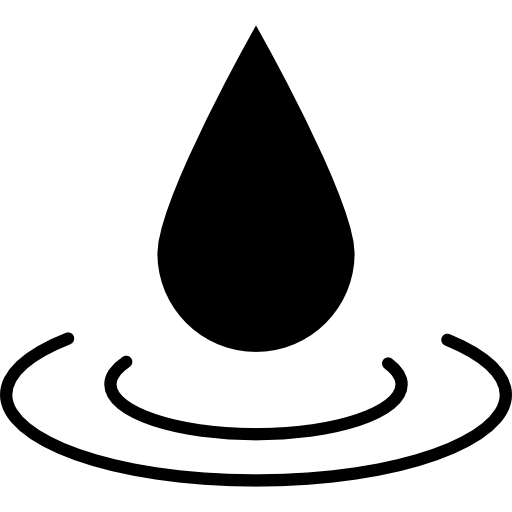
\includegraphics[width=0.15\linewidth]{Chapter5/Figs/hydro}

\vfill
This study was conceived by ADL with input from DAK. DAK and MGT provided floristic plot data and edaphic data. ADL conducted soil moisture sampling and collected supplementary floristic and edaphic data. FH and ADL developed latent variable co-occurrence models. ADL conducted analyses and wrote the manuscript, with contributions from DAK, MGT \& FH. 

\end{center}
\newpage

\section{Abstract}

1. Theory suggests spatial heterogeneity can facilitate species co-occurrence at fine-scales, but environmental data is rarely collected at sufficiently high resolution to test this empirically. While there is emerging evidence subtle variation in soil hydrology represents a fundamental fine-scale niche axis within plant communities, this is largely derived from studies of soil hydrology in isolation from other environmental factors. 

2. We assessed the comparative importance of fine-scale hydrological niche differentiation for species co-occurrence using a high resolution study of soil hydrology and other edaphic variables, coupled with a long-term (24 years) dataset of herbaceous plant plots in a heathland community in southeast Australia. 

3. For the analysis, we employed novel latent variable models (LVMs), which offer an explicit, model-based approach to partitioning out the different drivers of species co-occurrence patterns. While the regression component of an LVM models the species-specific environmental responses, the latent variable component can be used to identify residual patterns of co-occurrence, which may be attributable to unmeasured factors and/or biotic interactions.     

4. Relative to a host of plant resources, non-resource factors and `unmeasured' latent variables, soil hydrology emerged as the best predictor of negative co-occurrences within the community, with the dominant species exhibiting strongly differentiated responses across a comparatively narrow moisture gradient. Nevertheless, strong species-specific responses to environmental variability only emerged at scales greater than those at which plants may be expected to compete for resources, throwing doubt on the direct role of spatial heterogeneity as a mechanism for local-scale coexistence. 

5. \textit{Synthesis}. This study confirms the vital role of hydrological niches for the maintenance of within-community plant diversity, but also highlights the need for more rigorous analysis of scale dependencies to better understand the underlying coexistence mechanisms at play. In addition, it illustrates the inferential gains made possible with model-based approaches to the analysis of species co-occurrence.

\newpage

\section{Introduction}

Spatial environmental heterogeneity is widely recognised to play a fundamental role in driving broad-scale patterns of diversity and compositional turnover. The underlying mechanisms are diverse, but include wider niche space, more refuges from adverse conditions, and stronger selection for evolutionary diversification \citep[reviewed in][]{Stein2014}. At finer, within-community scales, however, the extent to which heterogeneity explains observed patterns of species co-occurrence is less clear. In spite of a wealth of theory suggesting that `variation dependent' coexistence mechanisms may be pervasive \citep{Chesson2000, Amarasekare2003, Snyder2004}, the empirical evidence is surprisingly sparse \citep[but see][]{Sears2007, Fridley2011}. One explanation for this disconnect between theory and data is that environmental heterogeneity is rarely examined at sufficiently high resolution to evaluate its influence on within-community scale patterns of diversity \citep{Adler2013, Kraft2014}. More specifically, in observational studies, the local environment is typically treated as spatially homogenous, with coexistence attributed to variation independent processes such as resource partitioning, the temporal storage effect or neutral dynamics \citep{Chesson2000, Hubbell2001}. Matching this missing fine-scale environmental data with floristic observations will aid identification of the proximal causes of plant diversity maintenance at within-community scales.

Species coexistence arising through spatial heterogeneity is contingent on multiple criteria, but the most fundamental prerequisite of these is the presence of different species-specific responses to the environment \citep{Chesson2000, Silvertown2004}. More specifically, for a given spatially heterogeneous environmental variable to operate as a plant niche axis, and thus reduce niche overlap, species need to favour different regions of that variable. It follows that the spatial structure of the variable needs to exhibit sufficient temporal stability such that individuals may germinate, reach reproductive maturity, and preferably build-up a local population before the environment changes \citep{Grubb1977, Chesson2000, Muko2000, Amarasekare2003}. Of the vital plant resources, water in the form of soil moisture has repeatedly been shown to exhibit a high degree of temporal stability, whereby across fine-scales, localities may often be consistently ranked on the basis of their soil water content \citep{Vachaud1985, Cassel2000, Pachepsky2005}. As such, given the essential physiological role of water in plant function, and the vast array of plant adaptations to water stress and uptake, there is a strong \textit{a priori} expectation that in some systems fine-scale variability in soil moisture may provide one of the more important axes of niche differentiation \citep{Silvertown2015}. 

Whilst ecologists have long been aware of the tendency for plant species to segregate along strong soil moisture gradients \citep{Pickett1978}, evidence that subtle variation in soil moisture can also moderate co-occurrence patterns is only just emerging. \citet{Silvertown1999} first demonstrated fine-scale hydrological niche differentiation across topographically invariant landscapes in European wet meadows. More recently, \citet{Araya2011} underscored the potential generality of the phenomenon in \textit{Restio} dominated fynbos communities in the Cape Floristic region of South Africa. Given their combined taxonomic and geographic breadth, together the evidence from these two studies is compelling, and yet there remains a strong mandate for wider investigation. In particular, we know very little about the comparative strength of soil moisture relative to other important plant resources (e.g. nitrogen, phosphorous, organic carbon) as drivers of fine-scale plant co-occurrence patterns.


Whilst manipulative experimental approaches arguably have the greatest potential to disentangle underlying mechanisms in annual plant communities \citep[e.g.][]{Sears2007a, Godoy2014}, they are less amenable to perennial systems where individuals can take several years to reach reproductive maturity. Fortunately, recent advances in statistical methods and computing power have greatly enhanced the capacity of researchers to draw robust inferences from the kinds of purely observational datasets that are typical in studies of perennial communities. In particular, an emerging family of community-level model-based approaches have the potential to yield significant new insights \citep{FERRIER2006, Warton2014}. These include a subset of models which are specifically orientated towards disentangling patterns of co-occurrence and their abiotic and/or biotic drivers \citep{Ovaskainen2010, Pollock2014, Harris2015}. In contrast with conventional null-model based approaches, multivariate co-occurrence models \citep[also known as Joint Species Distribution Models (JSDM), after][]{Clark2013} provide a direct means of assessing shared environmental responses separately from other (abiotic and biotic) processes that may generate non-random patterns of co-occurrence. Furthermore, as they are built upon the standard regression framework of generalized linear models \citep{mccullough1989}, they facilitate more transparent and accurate representations of the statistical properties of the data \citep[e.g. overdispersion of counts,][]{Warton2012}, as well as provide a means of accounting for structural complexity and uncertainty in a hierarchical framework \citep{Cressie2009}.

In this study, we assessed the comparative importance of hydrological niche segregation for species co-occurrence, using a high resolution study of soil hydrology and other edaphic variables, coupled with a long-term (24 years) dataset of herbaceous plant plots in a coastal heathland community in southeast Australia. To this end, we modelled pairwise co-occurrence using an extension of the latent variable model \citep[LVM,][]{Skrondal2004} approach for model-based unconstrained ordination recently proposed by \citet{Walker2011} and \citet{Hui2014}. LVMs offer an explicit, model-based approach to partitioning out the different drivers of species co-occurrence patterns. In particular, the regression component of an LVM models the species-specific environmental responses, based on which we can evaluate the prevalence of species-specific responses to soil hydrology, in comparison with a range of other important plant resources and non-resource factors. The latent variable component of the LVM is used to identify the residual patterns of species co-occurrence, which may be attributable to unmeasured factors and/or biotic interactions.

If heterogeneity in fine-scale hydrology is an important niche parameter, we predicted species would exhibit strongly differentiated responses to the local soil moisture gradient, and that relative to other environmental variables, this would translate into large numbers of negative correlations between species. To evaluate the overall influence of the environment on patterns of species co-occurrence, we further examined the residual patterns of co-occurrence in an LVM including multiple environmental predictors in a single model. If the environment is the dominant force structuring patterns of negative species co-occurrence, we expected weak residual correlations induced by the latent variables. Conversely, if any unmeasured environmental factors and/or biotic processes are equally, or more, important than measured environmental factors, we expected strong correlations based on the latent variables. 

Given that observations of species distributions at fine spatial grains are known to be sensitive to stochastic processes \citep{Chase2014}, we performed our primary analysis on all plots from all censuses combined, whilst accounting for spatial and temporal non-independence in a hierarchical framework. This aggregation of census data collected over a long period of time not only served to minimize the masking affect of stochastic phenomena on underlying species-environment associations, but also to reduce measurement error that might arise from missed detections in any given single survey. Nevertheless, to aid interpretation and disentangle spatial and temporal processes, we additionally examined species species-specific responses at each individual census, as well as at a finer spatial scale to the main analysis.

\section{Materials and methods}

\subsection{Study area and floristic sampling}

Sampling was conducted in an area (approx. 4 ha) of fire-prone coastal heathland in Royal National Park, New South Wales, Australia. The herbaceous ground layer is dominated by species within the Restionaceae, Cyperaceae and Poaceae families, while the overstorey consists mainly of sclerophyllous shrubs within the Proteaeceae, Myrtaceae, Ericaceae and Fabaceae families \citep{KEITH2007}. The soils derive from a sandstone substrate, and tend to be low in nutrients, sandy and acidic. The topography is relatively flat, with minimum and maximum elevations of 67 and 71 metres respectively. A previous study found that terrain-based hydrological models provided poor estimates of true soil moisture at the site \citep{Holman1999}, as is typical of low relief areas \citep{Anderson1980}.

Fifty-six 0.25 m$^{2}$ plots within the study area were sampled ten times over 24 years (1990-1994, 1999, 2002, 2007, 2011 and 2014). At each census, the abundance (number of stems) of all herbaceous species in each plot was recorded. The plots are spatially clustered into four groups of 14, with a mean distance of 211 metres between each cluster (min = 104 m; max = 323 m). Within each cluster, plots are spaced a mean distance of 18 metres apart (min = 5 m, max = 45 m). A fire in October 1988 burnt the entire site prior to the commencement of the study, with subsequent fires in January 1994 (all plots burnt) and January 2001 (14 plots in one cluster burnt).

We restricted our analysis to the most dominant species, where dominance was defined as those species present in at least 20\% of all 560 observations (56 plots x 10 censuses). Out of a total of 49 species, 12 met this criterion. The rationale for only considering the dominant species was both ecological and methodological. Firstly, we asserted \textit{a priori} that for any given environmental variable to be considered an important niche axis in the community, at least two of the dominant members should exhibit distinct responses to that variable. Secondly, the model-based framework we employed precluded the analysis of rare species for which too few data points were available.      


\subsection{Environmental sampling}

In March-May 2013, 56 100 cm access tubes for a PR2/6 soil moisture profile probe (Delta-T Devices: \url{http://www.delta-t.co.uk}) were installed within 10 cm of each plot. The probe is fitted with six sensors allowing for instantaneous soil moisture measurements at six depths (10/20/30/40/60/100 cm). After a two month settling-in period, soil moisture sampling commenced in early August 2013 and was repeated at monthly intervals until July 2014. At each monthly interval, three readings (x six depths) were taken at each plot, with the probe rotated through 120 degrees between each reading to account for any small scale variability in moisture at each depth.   

In addition to present day measurement of soil moisture, a range of edaphic variables known to be important for plant growth and survival have been sampled in the immediate vicinity of each plot on seven occasions spread across the sampling period (1991, 1993, 1994, 1995, 1999, 2002 and 2014). At each plot, 5-10 soil cores (diameter: 27 mm; length = 100 mm) were sampled randomly within 10 cm of the plot boundary. In each given sampling year, the cores from each plot were combined and analysed for a range of variables, including organic carbon (all years), ammonium nitrogen (NH$_{4}$) (all years excluding 1991, 1999 and 2014), nitrate nitrogen (NO$_{3}$) (all years excluding 1991), total iron (all years excluding 1991, 1995 and 2002), phosphorous (all years excluding 1991, 1995 and 2002),  conductivity (all years), pH (all years), cation-exchange capacity (CEC) (all years) and various exchangeable cations (Na, K, Ca, Mg \& Al) (all years).



\subsection{Data preparation}

Prior to inclusion in models, soil variables were evaluated for several criteria including sufficient spatial heterogeneity, relative temporal stability (a prerequisite for a spatial niche axis), and the absence of outliers. Both nitrate and exchangeable K were at such low levels that very little variability in their concentration could be detected, and were consequently excluded from the analysis. Of the remaining variables, nitrogen (ammonium), conductivity, exchangeable Na and exchangeable Ca were found to exhibit substantial temporal variability with rapid temporal decay in their spatial correlation (mean Spearman correlation coefficient between sample years = 0.23, 0.17, 0.20 \& 0.32 respectively) and so were also excluded.
%(see supplementary material for inter-census correlation matrices for all variables).
The mean value was then calculated for each of the remaining variables at each plot, following which outliers (never more than two) were excluded for several variables to avoid them having a disproportional influence on parameter estimates. The final set of variables included phosphorous, organic carbon, total iron, pH, cation exchange capacity, exchangeable Mg and exchangeable Al, as well as two measures of soil moisture detailed further below. 

In the absence of between year samples of soil moisture at each plot, the temporal stability of soil moisture at each depth was evaluated on the basis of the variability observed over the 12 month sampling period. 
The vertical profile (100, 200, 300, 400, 600 and 1,000 mm) for soil moisture exhibited a gradual decay in correlation such that values at 100 mm were near independent of those at 1,000 mm (r = 0.09), while those at intermediate depth fell along a spectrum between these two extremes. As a result, we subsequently restricted further evaluation of soil moisture to these two depths, one representing `shallow' near surface soil moisture (100 mm) and one representing `deep' soil moisture (1,000 mm). To evaluate the temporal stability of soil moisture, both in terms of relative spatial structure and absolute levels, we considered the mean Spearman rank correlation coefficient of all pairwise monthly comparisons (relative stability), and the overall standard deviation in mean monthly soil moisture (absolute stability). Deep soil moisture was highly stable in both relative and absolute terms, with mean pairwise correlation between months, r = 0.96, and standard deviation in average monthly soil moisture = 1.017. Shallow soil moisture was only slightly less stable with mean pairwise correlation between months = 0.86, and standard deviation in average monthly soil moisture = 4.7. The high Spearman rank coefficients observed at both depths indicate high temporal stability in the relative spatial structure of soil moisture at the study site, whilst the increase in stability with depth is consistent with previous work \citep{Cassel2000}. As such there is strong evidence that the spatial structure of soil moisture observed over the 12 month monitoring period is typical of that which would have been observed throughout the floristic sampling period. %This persistent pattern is further supported by two previous surveys ('96 and '99) of shallow soil moisture across a $~$40 m resolution grid partially overlapping the study area, which despite significant uncertainty in the exact location of samples between surveys, were comparatively well correlated (Spearman's \textit{r} = 0.356, \textit{p} $<$ 0.05) \citep{Holman1999}. 
Furthermore, variability in monthly rainfall over the 12 month monitoring period (sd = 57.3) was near that observed for the entire period since floristic surveys began in 1990 (sd = 78.4). The final per plot measurements of deep and shallow soil moisture were obtained by averaging across all 12 monthly samples. Notably, average shallow soil moisture was unrelated to elevation (\textit{p} = 0.832), while deep soil moisture was weakly, and positively related (R$^2$ = 0.1031 \textit{p} = 0.0179), indicating a very slight increase in deep soil moisture with increasing elevation. 

Finally, to obtain an estimate of light availability in the final year of sampling, bottom-up canopy photographs were taken over two days in March 2014. At each plot, two replicate photographs were taken using an SLR camera with a fish-eye lens positioned facing directly upwards on a level surface in an east-west orientation. The images were then digitally converted to black and white based on an automatic threshold using the GIMP graphics editor (www.gimp.org), and the ratio of black to white pixels (representing vegetation cover) was quantified.  The two counts for each plot were then averaged.

\subsection{Model design}

We used a novel approach to analyzing co-occurrence patterns based on latent variable models (LVM). LVMs can be regarded as an extension of factor analysis \citep{knott1999} to non-normally distributed responses. For each of the nine environmental predictors (excl. light availability), we ran three different LVMs: one leveraging all plots and censuses combined (full model); one for each of the four clusters of plots (individual cluster model) to infer to what extent patterns observed for the full dataset were driven by variation within or between clusters; and one for each of the ten individual censuses (individual census model) to evaluate the temporal stability of pairwise co-occurrence patterns. Additionally, we fitted an LVM for the full dataset which included multiple environmental predictors (excl. light availability) in order to identify remaining patterns of co-occurrence after accounting for the environment. Due to collinearity (\textit{r}  $>$ 0.7) amongst several variables, three variables (pH, CEC and Exchangeable Mg) were left out of the multi-predictor model. We also fitted a single LVM for species co-occurrence as a function of light availability for 2014 only. For the individual cluster models, we restricted our analysis to those species that occurred in at least 20\% of all plots in each cluster over the 10 censuses (as was done for the full model). For the individual census point models, the criterion was relaxed to 10\% of all plots at each time-step. A schematic summarizing the relationship between the different models and associated analyses (detailed further below) is provided in Fig. \ref{fig:schem}.

\begin{figure}[H]
\centering
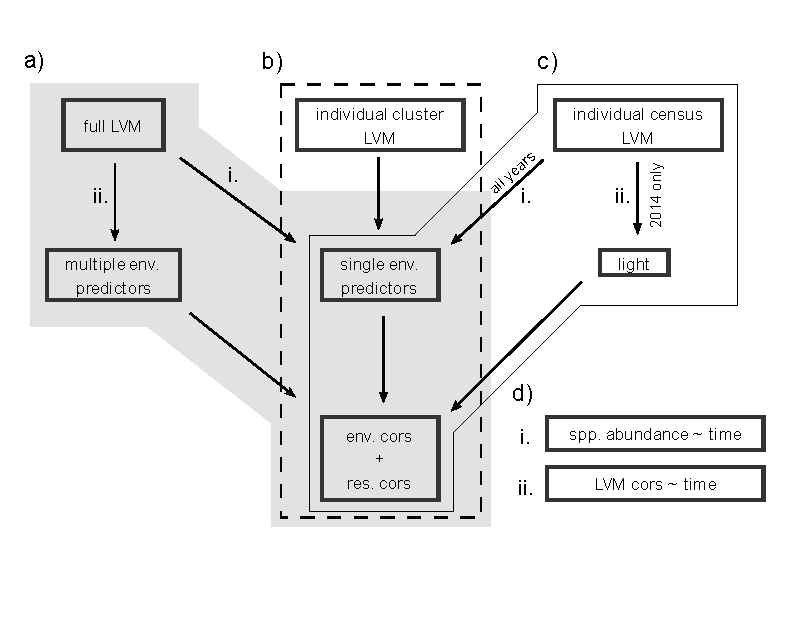
\includegraphics[width=1.0\linewidth]{Chapter5/Figures/schem2}
\caption{Schematic summary of core analysis. Environmental and residual correlations calculated  for: a) LVMs fitted to the full  dataset for i) each of the nine environmental predictors  independently, and ii) for multiple predictors in a single model; b) LVMs fitted to each individual cluster for each predictor independently; and c) i) LVMs fitted to each census for each predictor independently (all census years), and ii) additionally for light in 2014. Supplementary GAMMS were fitted for: d) i) species abundance as a function of time for comparison with the residual correlations from the multiple predictor model, and ii) for environmental and residual correlations from the individual census LVMs as a function of time.}
\label{fig:schem}
\end{figure}

Similar to other co-occurrence models such as JSDMs \citep[e.g.,][]{Ovaskainen2010, Clark2013, Pollock2014}, the extent to which species exhibit distinct environmental responses was inferred through a fitted regression model, specifically using the framework of generalized linear models. However, instead of employing an unstructured covariance matrix to account for the missing environmental covariates and/or biotic interactions \citep[as was done in][for instance]{Ovaskainen2010, Pollock2014}, LVMs utilize latent variables as a parsimonious means of modelling residual species correlation \citep[see also][]{Harris2015}. As such, we use the term `residual' in reference to remaining patterns in the data after accounting for one or more predictors, rather than in terms of its definition in the context of residual analysis. 

Our model can be regarded as an extension of the LVM proposed for model-based unconstrained ordination in \citet{Hui2014}, and can be written in the following hierarchical form:

\begin{align} \begin{aligned}[c] \label{eqn:basiclvm} 
\text{Responses:} &\quad [y_{ij} | \bm{u}_i, \bm{x}_i] \sim \text{Neg-Bin}(y_{ij}; \mu_{ij}, \phi_j) \\
&\quad \log(\mu_{ij}) = \eta_{ij} = \bm{x}'_i \bm{\beta}_j + \bm{u}'_i \bm{\lambda}_j \\
\text{Latent Variables:} &\quad [\bm{u}_{i}] \sim \mathcal{N}(\bm{0},\bm{I}) \\ 
\text{Priors:} &\quad [\bm{\beta}_j] \sim \mathcal{N}(\bm{0},c_0\bm{I}), \; [\bm{\lambda}_j] \sim \mathcal{N}(\bm{0},c_0\bm{I}), \; [\phi_j] \sim \text{Unif}(0,c_1), 
\end{aligned} \end{align}

where $`\sim'$ denotes ``is distributed as'', $\mathcal{N}(\cdot,\cdot)$ denotes a multivariate normal distribution with mean and covariance matrix given by the first and second arguments respectively, $\text{Unif}(0,c_1)$ denotes a uniform distribution with minimum zero and maximum $c_1$, and $\bm{I}$ denotes an identity matrix. To elaborate, $y_{ij}$ denotes the observed count for species $j$ at site $i$, and is assumed to come from a negative binomial (Neg-Bin) distribution with mean $\mu_{ij}$ and species-specific overdispersion parameter $\phi_j$. We used a negative binomial distribution as it exhibits a quadratic mean variance relationship, $\text{Var}(y_{ij}) = \mu_{ij} + \phi_j\mu^2_{ij}$, which allowed us to explicitly account for overdispersion present in the species counts.

Using a log-link function, the mean $\mu_{ij}$ was regressed against two sets of variables. Firstly, a vector of explanatory variables for each site, $\bm{x}_i$, which included an intercept term, environmental covariates (e.g. soil moisture), a fixed effect for the four clusters of plots to account for spatial non-independence within clusters (full and individual year models), and a random effect (intercept) for plot to account for temporal non-independence (full and individual cluster models). In order to account for unimodal species responses as predicted by niche theory \citep{Austin2002}, quadratic terms were included for the environmental covariates in each model. The second set of variables comprised a vector of two latent variables for each site, $\bm{u}_i = (u_{i1},u_{i2})$, which were assumed to be drawn from independent, standard normal distributions. The species-specific regression coefficients $\bm{\beta}_j$ and $\bm{\lambda}_j$ describe how the mean changes as a function of the explanatory and latent variables respectively.  

The key element in the LVM in equation (\ref{eqn:basiclvm}) are the latent variables $\bm{u}_i$, which can account for any residual correlation between species not attributable to spatial heterogeneity in the measured environmental covariates $\bm{x}_i$. This correlation may be driven by biotic interactions such as competition (negative) or facilitation (positive), or alternatively to missing predictors, where $\bm{\lambda}_j$ are the coefficients corresponding to these missing predictors. In addition, in our full model which combines multiple censuses, residual correlation may arise due to negatively or positively correlated fluctuations in species abundance through time. If unaccounted for, missing covariates, ecological interactions or temporal correlation will induce residual correlation between species which can potentially lead to erroneous inference. Latent variables offer an attractive approach to dealing with this issue. In particular, they require significantly fewer parameters to model species residual correlation compared to the unstructured (full rank) correlation matrices used by \citet{Ovaskainen2010} and \citet{Pollock2014}. Finally, note that more than two latent variables could have been used, although our preliminary testing with this dataset suggested that two was sufficient to characterize the main patterns of species residual correlations. 

We used Bayesian Markov Chain Monte Carlo (MCMC) methods to estimate the LVMs, with sampling performed through JAGS v3.4.0 \citep{plummer2003jags} using the package R2jags v0.03-08 \citep{su2012r2jags} in \texttt{R} v3.1.1. We assigned uninformative priors for all parameters, $\bm{\beta}_j, \bm{\lambda}_j$ and $\phi_j$, by setting $c_0 = c_1 = 100$ in equation (\ref{eqn:basiclvm}). For the full and individual cluster models, we also assigned an uninformative uniform prior for the variances of the random effect for plot. For each LVM fitted, we ran three chains with a burnin period of 10,000 iterations followed by 100,000 iterations with a thinning lag of 50 for each chain. This produced a final combined sample of 6000 MCMC samples for each LVM. We assessed parameters to have converged when traceplots were well mixed and the Gelman-Rubin statistic was below 1.1.

\texttt{R} code demonstrating the fitting and analysis of latent variable models of co-occurrence is provided in Appendix D.

\subsection*{Model inference and supplementary analysis}

After fitting the LVMs, in order to visualize patterns of co-occurrence arising from the different environmental factors, we calculated two types of correlation matrices. The first was constructed by calculating, for any two species, the correlation between their fitted values $\bm{x}'_i \bm{\beta}_j$ (across all plots). This is the same as equation (4) in \citet{Pollock2014}, with the resulting matrix representing the correlation between species that can be attributed to a shared/diverging environmental response. The second type of correlation matrix was calculated using the latent variable coefficients, $\bm{\lambda}_j$, also known as factor loadings. Specifically, if we let $\bm{\Lambda}$ be the two-column matrix formed by stacking the factor loadings on top of each other, then a covariance matrix is obtained as $\bm{\Lambda}\bm{\Lambda}'$ from which the residual correlation matrix can be calculated. This second residual correlation matrix represents the correlation between species that may be attributable to biotic interactions or missing environmental covariates. Since Bayesian MCMC estimation was used, the correlation between fitted responses was calculated for each MCMC sample, which made it possible to obtain a posterior distribution for each cell of the environmental and residual correlation matrix. As such, correlation `significance' was evaluated on the basis of the 95\% credible intervals for the posterior mean excluding zero. 


Having extracted environmental and residual correlation matrices for each environmental factor in each of the three model types (full, individual cluster, individual census point), we assessed the importance of each factor as a niche axis on the basis of two criteria: i) the number of significant negative pairwise environmental responses, where significance is defined as 95\% credible intervals that don't cross zero; and ii) the minimum number of species that need to be excluded to remove all negative pairwise responses, referred to in network theory as the minimum vertex cover. In this application, the minimum vertex cover quantifies the extent to which a given number \textit{n} of negative pairwise environmental responses is driven by one species exhibiting a different response to all other species, or at the other extreme consists of completely unique species pairs. In the former case, only one species need be excluded to remove all negative correlations whereas in the latter case $\textit{n}$ species must be removed. As such, with 12 species, if all 66 unique pairs exhibit significant negative correlations (an implausible scenario necessitating extremely narrow niche breadths), 11 would need to be excluded. In addition to quantifying negative pairwise environmental responses, we also counted the number of positive (shared) environmental responses to evaluate the extent to which a given environmental factor influences the fine-scale distribution of species even in the absence of any clear niche differentiation (e.g. if all species exhibit a similar response to the gradient). 

After considering species-specific environmental responses, we then examined the residual correlation matrix for each model, with particular emphasis on the full model including all of the environmental predictors, as this represents patterns of co-occurrence unexplained by all our measured predictors combined. To aid interpretation of the residual correlation matrix from the full multi-predictor model, we also fitted a generalized additive mixed model (GAMMs) for each species as a function of time, and compared the correlation in the fitted values from the GAMMs with the residual correlation matrix based on the full LVM model including multiple environmental predictors. The temporal GAMMs for each species were fitted using the MGCV package \citep{wood2012mgcv}, with a thin-plate spline smoother for time, a fixed effect for plot cluster, a random effect for plot, an AR(1) correlation structure nested within plot, and assuming a negative binomial error distribution with log link. If patterns in the residual correlation matrix of the full model are largely a product of temporal correlation (negative or positive) in species responses, we expected a strong correlation with the fitted value correlation matrix derived from the individual GAMMs. Correlation between the two matrices was assessed via a Mantel test. Note that the GAMM for one species, \textit{Empodisma minus}, failed to converge (most likely due to overdispersion), and as a result had to be excluded from the temporal analyses.

To investigate temporal trends in environmental and residual correlations, we also fitted GAMMs for mean pairwise environmental and residual correlation as a function of time for all variables combined. Each model included a thin-plate spline smoother for time, a random effect for environmental variable and an AR(1) correlation structure nested within environmental variable. Owing to the mean correlations values being consistently positive and right skewed, we used a gamma error distribution with a log link function. To correct over-smoothing observed in the residual correlation trends model, the maximum number of degrees of freedom was reduced from 9 (package default) to 4.

Finally, we performed \textit{post-hoc} exploratory analysis of the differences in species response to soil moisture with their pairwise differences in two readily available aboveground traits, plant height and seed mass. In each case, we used a Mantel test to compare pairwise difference in soil moisture (-1 x environmental correlation) with pairwise trait differences, and visualised the relationship with scatterplots.    

\section{Results}

Of the nine environmental variables considered independently in each of the single-predictor models for the full dataset, all but pH produced significant negative correlations due to diverging species-specific responses (Fig. \ref{fig:networkplots-negfull}). Deep soil-moisture was associated with both the largest number of negative correlations (18) and the largest number of node removals required to eliminate all negative correlations (4). As is to be expected given such strong correlations, the 12 species displayed a range of differentiated responses to the deep soil-moisture gradient, with some increasing monotonically (or near monotonically) towards the extremes of the gradient (e.g. \textit{Xanthorrhoea resinosa}, \textit{Haemodorum corymbosum} and \textit{Entolasia stricta}), whilst others exhibited unimodal peaks closer to the middle of the gradient (e.g. \textit{Ptilothrix deusta}, \textit{Empodisma minus} and \textit{Xyris gracilis}) (Fig. \ref{fig:responsefig_cred}). Exchangeable aluminium was associated with the second largest number of negative correlations (17), followed by organic carbon (11), shallow soil-moisture and total iron (10), exchangeable magnesium (6), cation exchange capacity (3), and phosphorous (1) (Fig. \ref{fig:networkplots-negfull}). Whilst pH was not associated with any negative pairwise correlations, 27 species pairs exhibited significant positive correlations to pH. Deep soil-moisture was associated with the second highest number of significant positive correlations, followed by exchangeable aluminum and exchangeable magnesium (21), organic carbon (18), shallow soil-moisture (17), total iron (16), cation exchange capacity (12), and phosphorous (8) (see Fig. S5.1 in Appendix D).
 
 \begin{figure}[H]
 \centering
 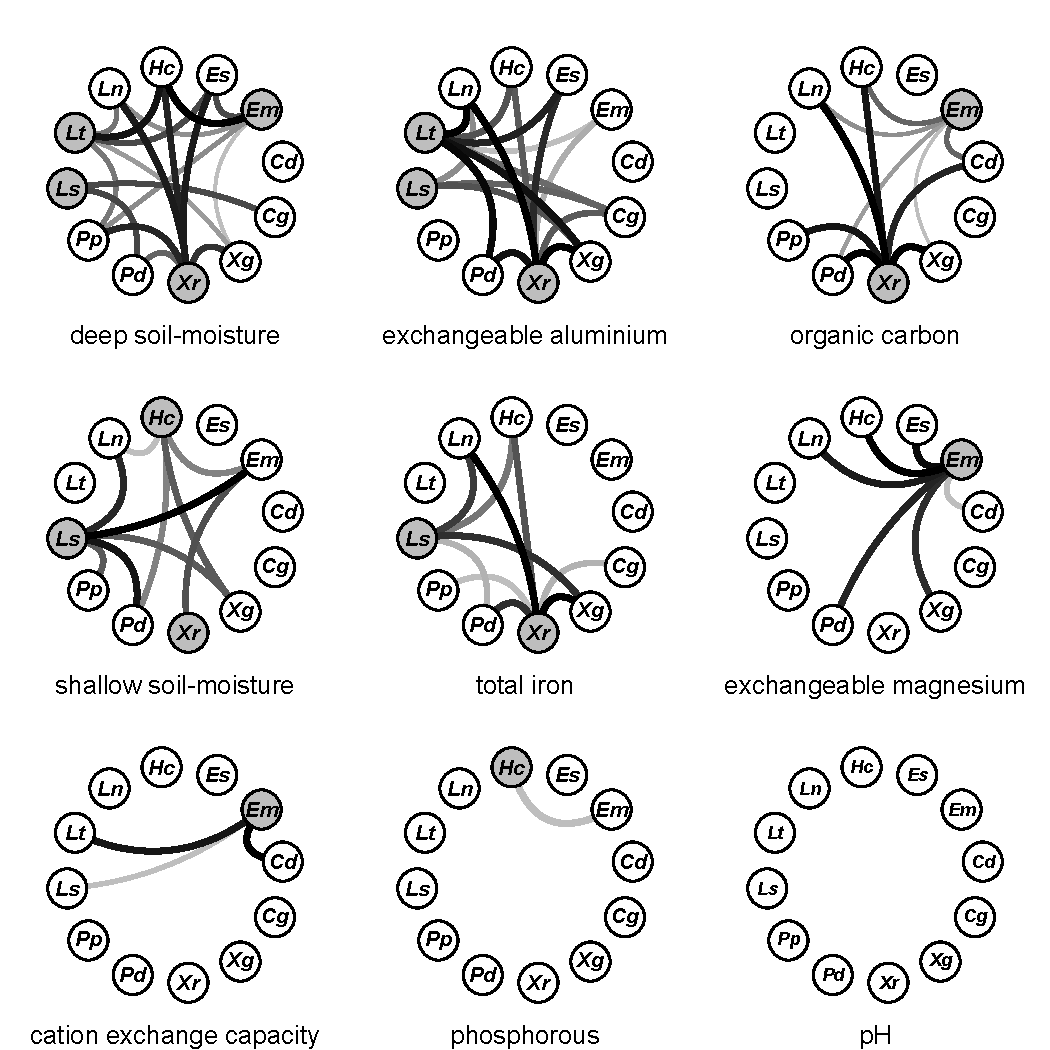
\includegraphics[width=1.0\linewidth]{Chapter5/Figures/networkplots-negfull}
 \caption{Negative pairwise species correlations to the environment derived from single-predictor LVMs for the full dataset. Connecting lines between species nodes denote negative mean posterior correlations with credible intervals excluding zero. Line colour and thickness indicates the strength of the negative correlation where darker and thicker lines are closer to -1. Nodes shaded grey indicate the minimum vertex cover, i.e. the smallest combination of species that need to be removed to break all negative associations (note that while the minimum number has a single solution, the species composition making up the minimum vertex cover set can vary). Species node labels combine the first letters of the genus and specific epithet given in full in Fig. \ref{fig:responsefig_cred}.}
 \label{fig:networkplots-negfull}
 \end{figure}
 
 \begin{figure}[H]
 \centering
 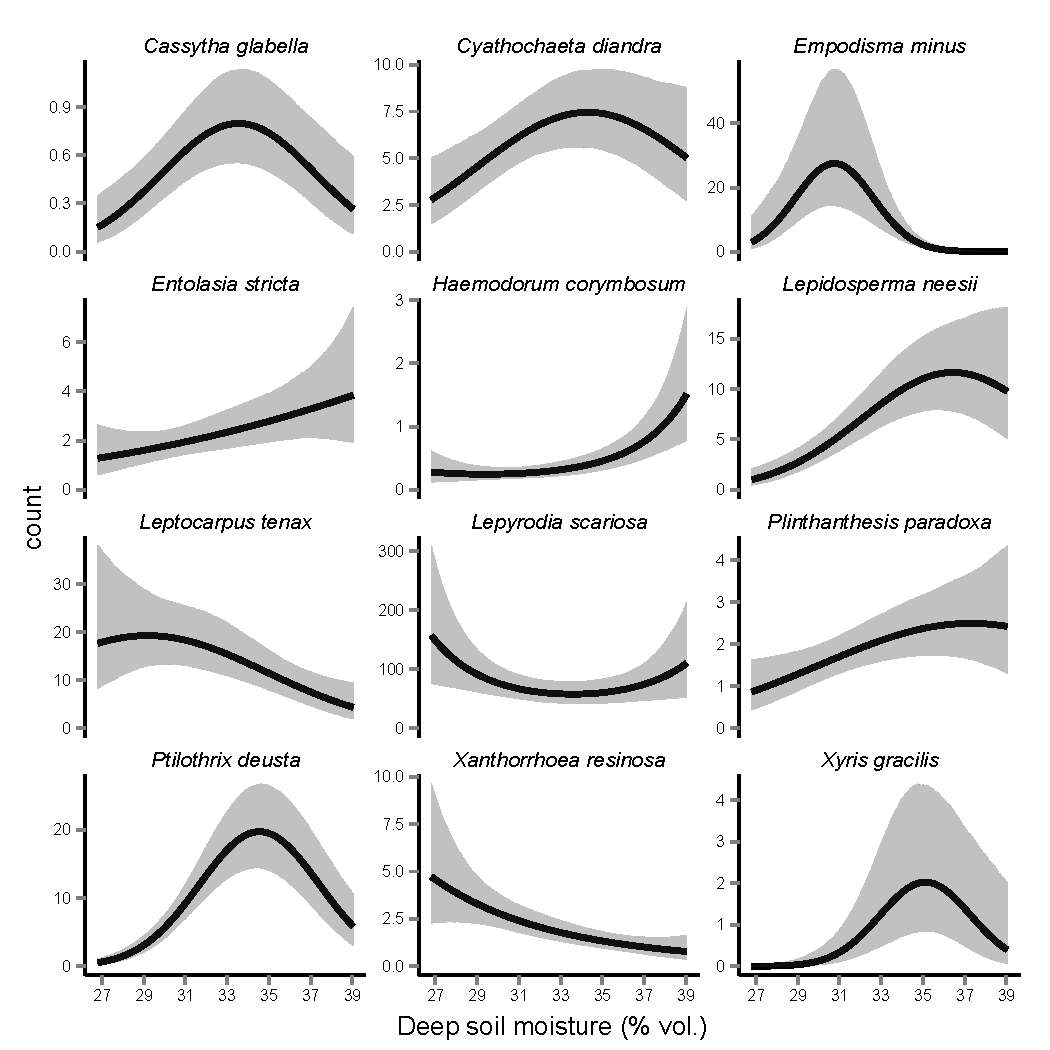
\includegraphics[width=1.0\linewidth]{Chapter5/Figures/responsefig_cred_mcmc}
 \caption{Species specific responses to the deep soil-moisture gradient. Fitted values derived from regression parameter estimates from the deep soil-moisture LVM (full dataset). Shaded region denotes 95\% credible intervals.}
 \label{fig:responsefig_cred}
 \end{figure}



Residual correlations based on single-predictor LVMs fitted to the full dataset were strongly associated with each other, and with residual correlations from the multi-predictor model (\textit{r} = 0.68-0.97). As such, the consistency of the observed residual correlations suggests a potentially important variable was not accounted for in any of the LVMs. Nevertheless, most of the significant correlations in the residual correlation matrix  of the multi-predictor model were positive (23) rather than negative (2), thus negating the probability that an important fine-scale niche axis was omitted from our analysis (Fig. \ref{fig:multiresid}). Furthermore, a substantial portion of the residual correlation appears to be attributable to shared and differentiated temporal responses between species, with the residual correlation matrix from the multi-predictor model being moderately associated with the temporal response correlation matrix derived from the temporal models (Mantel test \textit{r} = 0.43) (see Fig. S5.2 for smoothed species responses through time).



\begin{figure}[H]
\centering
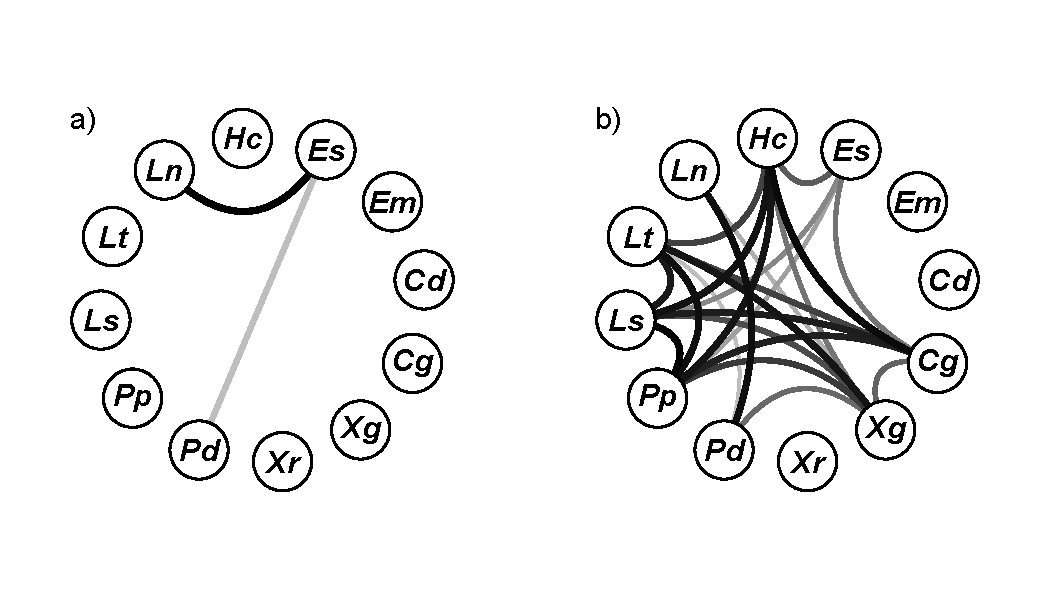
\includegraphics[width=0.7\linewidth]{Chapter5/Figures/multiresid}
\caption{Negative (a) and positive (b) pairwise residual correlations derived from the multi-predictor LVM for the full dataset. Connecting lines between species nodes denote posterior correlations with credible intervals excluding zero. Line colour and thickness indicates the strength of the correlation where darker and thicker lines are closer to $|1|$. Species node labels combine the first letters of the genus and specific epiphet.}
\label{fig:multiresid}
\end{figure}



Relative to the models run on the full dataset, the number of significant negative correlations due to diverging environmental responses between species was considerably smaller for models run on each individual cluster (plots separated by 5-45 metres). As such, most of the observed patterns of co-occurrence in the full models appears to be driven by environmental variation over spatial scales of 10s of metres, rather than metres (i.e. between clusters rather than within clusters). The one exception to this pattern was for phosphorous, which exhibited a relatively high number of significant negative co-occurrence associations in three of the four clusters. Notably, a substantial number of species did exhibit negative pairwise associations in the residual correlation matrices for at least two of the clusters, suggesting that biotic interactions may still influence co-occurrence at within-cluster scales (see Table S1).

The number of significant negative pairwise associations in species environmental response was also comparatively small for the individual census models. It is notable however that even if we ignore `significance' criteria, the sign of each pairwise species association is largely consistent with those observed for the single predictor models for the full dataset. In addition, the models for each individual census provide insight into the relative dominance of positive and negative interactions through time. Whilst there were no obvious trends in mean environmental correlation through time, residual correlations underwent a conspicuous upwards positive trend in the second half of the sampling period (Fig. \ref{fig:temptrends}). Pairwise species associations derived from the single LVM fitted for light availability in 2014 were almost universally positive, with all but one species (\textit{Xanthorrhoea resinosa}) being more abundant in less shaded locations. 

\begin{figure}[H]
\centering
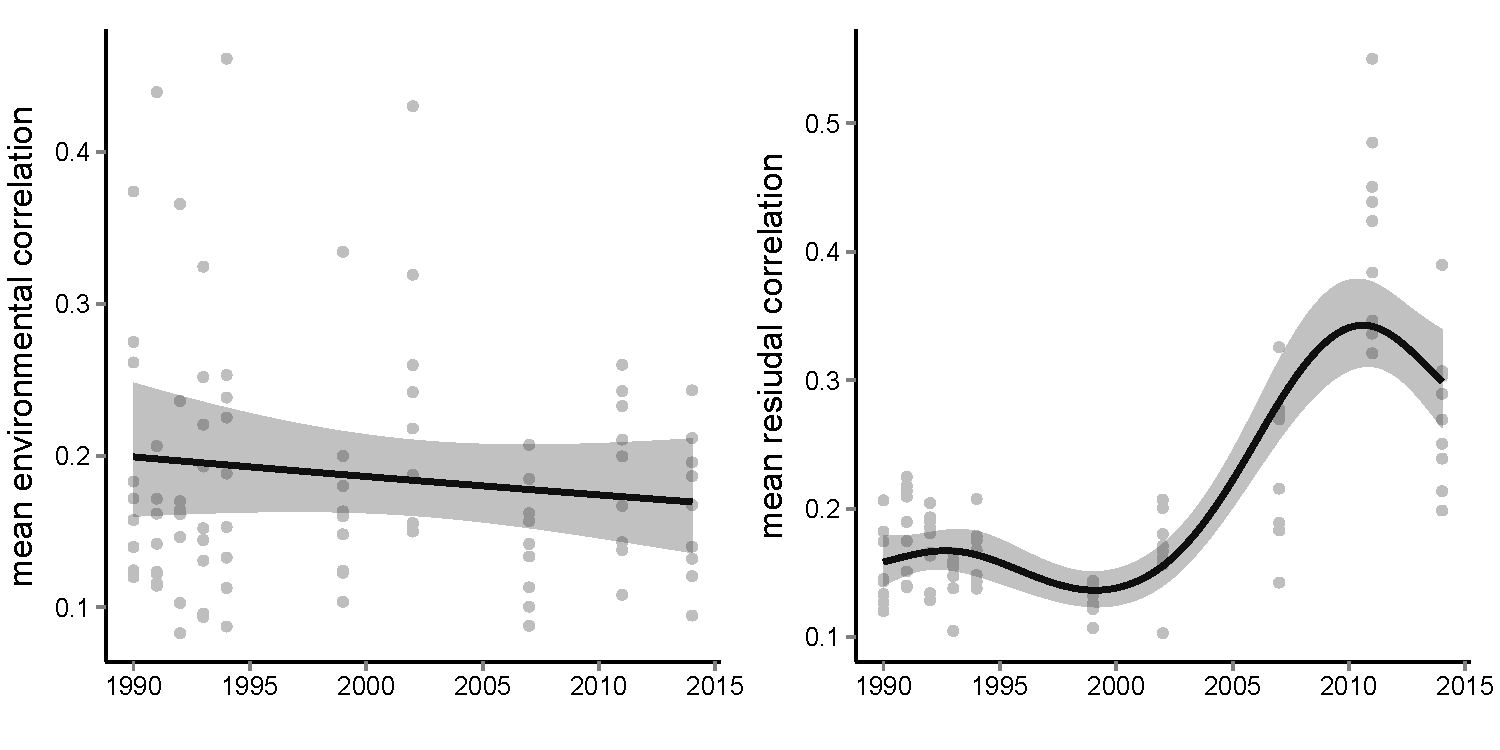
\includegraphics[width=1.0\linewidth]{Chapter5/Figures/temptrends}
\caption{Trends in mean environmental (left) and residual (right) correlation through time. Trend lines obtained with thin-plate splines in a GAMM framework (see main text for model fitting). Shaded region represents 95\% confidence intervals.}
\label{fig:temptrends}
\end{figure}



Differences in species pairwise responses to deep soil moisture were moderately positively related to pairwise difference in plant height (\textit{r} = 0.6259, \textit{P} = 0.002) but unrelated to differences in seed mass (\textit{r} = -0.1176, \textit{P} = 0.809) (Fig. \ref{fig:traits_diffs}). 

\begin{figure}[H]
\centering
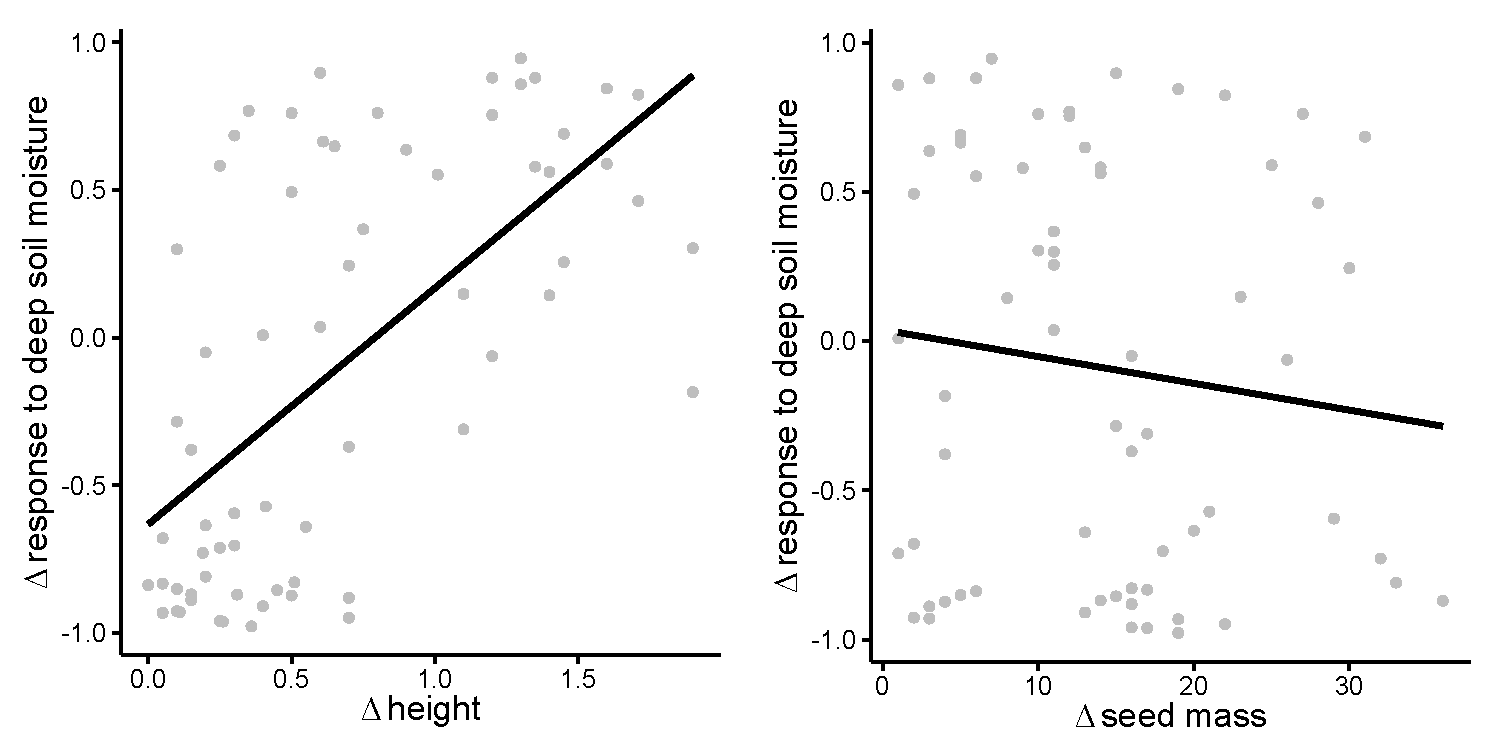
\includegraphics[width=1.0\linewidth]{Chapter5/Figures/traits_diffs}
\caption{Scatterplots of pairwise differences in species responses to deep soil moisture (-1 x environmental correlation) in relation to pairwise difference in plant height (left) and seed mass (right). Lines of best fit obtained from linear models.}
\label{fig:traits_diffs}
\end{figure}

\section{Discussion}

The notion that fine-scale spatial environmental variability may foster plant species coexistence is founded upon a rich body of theory \citep{Chesson2000, Amarasekare2003, Adler2013}, and yet empirical efforts to establish which, if any, environmental factors are associated with strong patterns of fine-scale niche differentiation are surprisingly sparse. We found strong empirical support for the hypothesis that differentiation along hydrological gradients represents one of the most important fine-scale plant niche axes at within-community scales \citep[\textit{sensu}][]{Silvertown2015}. On the basis of multiple criteria, deep soil moisture emerged as the single best predictor of negative co-occurrence patterns (Fig. \ref{fig:networkplots-negfull}), with the dominant community members exhibiting strongly differentiated responses across a comparatively narrow moisture gradient (Fig. \ref{fig:responsefig_cred}). Together with several earlier studies \citep[e.g.][]{Silvertown1999, Araya2011}, these results are amongst the first to demonstrate hydrological niche differentiation in the absence of significant topographical complexity. Furthermore, they highlight the robustness of the hypothesis when confronted with a comprehensive set of alternative prospective niche axes.

The adoption of a latent variable modelling framework enabled us to not only evaluate the comparative importance of each environmental factor, but also to determine the likelihood that an important factor was unaccounted for. Given that the residual correlation matrix from the multi-predictor model was dominated by positive pairwise associations, we can be confident that we accounted for the most important factors driving niche segregation amongst the dominant community members (Fig. \ref{fig:multiresid}). As such, our approach allows robust conclusions about the relative importance of soil hydrology not only with respect to measured variables but also unmeasured variables. Notably, a considerable portion of the residual correlation from the multi-predictor model appeared to be attributable to both positive, and to a lesser extent negative, temporal correlations in species peak abundance. These in turn appear to largely reflect differential interspecific temporal responses to fire events in 1988, 1994 and 2001 (Fig. S5.2). As such, with time-series data, co-occurrence models may also be used to draw inferences on successional processes and temporal niche partitioning. 

While the results provide strong evidence for fine-scale hydrological niche differentiation, the extent to which hydrological niches provide opportunities for local-scale species coexistence is to a large extent contingent on the scale at which the community is defined \citep{Amarasekare2003, Adler2013}. For instance, in the current study, negative co-occurrence patterns associated with the deep soil moisture gradient were only detectable when comparing plots across clusters separated by 100-320 metres. Similarly, \citet{Silvertown1999} made what is probably the strongest case for hydrological niches to date on the basis of plots dispersed across 10's of hectares, whilst even the ca. 50 x 50 metre plots of \cite{Araya2011} presumably allowed for individuals to be spaced as much as 70 metres apart. In contrast, \citet{Fridley2011} reported species-specific responses to microsite variation in soil depth in 3 x 3 metre plots in a limestone grassland, but this appeared to be unrelated to soil water potential. As such, the evidence for hydrological niches at the local scale within which neighbouring plants directly compete for resources arguably remains relatively weak. This conclusion would be in line with the dominant paradigm in community ecology that negative patterns of co-occurrence at the local scale are predominately indicative of competitive exclusion \citep[][but see Fridley \textit{et al.} 2011]{Gotelli2002}. Indeed, only phosphorous exhibited more than six negative pairwise associations (compared with just one for the full dataset) in any one plot cluster (Table S5.1). In contrast, the residual correlation matrices for two plot clusters exhibited a relatively large number of negative associations, which do not appear to be driven by any of the measured environmental factors. Nevertheless, even in the absence of localised spatial partitioning of resources, hydrological niches may still promote local coexistence via source-sink dynamics and spatial storage effects \citep{Shmida1984, Amarasekare2003, Snyder2004}. This will arise when species are able to disperse from favourable to less favourable locations at a sufficiently high rate to offset locally negative population growth rates and thus prevent local extinction \citep{Snyder2004}. Since monitoring began in the current study, all but one species has been recorded at all four clusters, suggesting that most of the dominant community members do indeed regularly disperse to and establish in locations where they are less competitive. It is also notable, that within short distances ($<$100 m) of our study plots, the topography is more varied, and as such may provide nearby opportunities for even finer scale hydrological niche differentiation. 

In contrast to the individual plot cluster models, the lack of strong negative environmental correlations in the individual census models appears to be an artefact of low power, particularly given that the raw correlation values corresponded closely with those from the full model. Nevertheless, it is interesting to note that whereas mean environmental correlations were relatively static through time, residuals correlations exhibited a strong upwards trend towards more positive values (Fig. \ref{fig:temptrends}). This trend most likely reflects a shared environmental response to increased overstorey shading, as indicated by the observed positive response of the majority of species to light availability in the most recent 2014 census. In a previous study from the same site, \citet{Letten2014a} described an increase in functional and phylogenetic similarity of community members through temporal succession consistent with this observation.

Our focus was on negative environmental correlations, but positive correlations also provide insight into other aspects of community assembly. For instance, positive correlations in species responses were highest for soil pH, suggesting pH may be a useful predictor of local richness patterns, whilst also acting as niche axis over larger spatial scales. It is also notable that although this system is typically associated with low-pH adapted species, many of the dominant herbaceous community members exhibited a positive response to the pH gradient (data not shown). As such, it would be interesting to explore the extent to which rarer species exploit this apparently `unoccupied' niche space within the landscape, particularly given the known importance of soil pH for plant community structure in other systems \citep{Laliberte2014}.

Although a comprehensive examination of trait-environment relationships was beyond the scope of this study, comparisons of species pairwise differences in seed mass and plant height relative to hydrological niches differences still proved informative. Whereas differences in seed mass, which may be associated with survival from drought stress \citep{Perez-Harguindeguy2013}, were unrelated to hydrological niches, differences in plant height were strongly positively related with differences in species response to soil moisture (Fig. \ref{fig:traits_diffs}; cf. Fig 2c in Adler \textit{et al.} 2013). This appeared to be driven predominately by taller species (e.g \textit{Leptocarpus tenax} and \textit{Xanthorrhoeaa resinosa}) favouring drier areas of the deep soil moisture gradient, while shorter species (e.g \textit{Plinthanthesis paradoxa} and \textit{Xyris gracilis}) were more abundant in wetter areas. This we expect reflects the greater tolerance of shorter species to anaerobic conditions in periodically saturated sites. Given that soil moisture measurements at all depths were typically around, or above, the field capacity of sandy-loam soil ($\sim$23\% vol., \citealp{atwell1999plants}), this possibly reflects the greater tolerance of shorter species to low oxygen in periodically saturated sites. In addition it suggests fine scale variability in soil moisture may have important implications for the structural complexity of standing vegetation.

Beyond differences in plant height and seed mass, it is notable that the dominant herbaceous members of the community actually exhibit remarkably similar phenotypes, with all but one of the twelve study species being a geophytic or hemicryptophytic monocot, and nine of the twelve belonging to just three families within the poales (\textit{Restionaceae}, \textit{Poaceae} and \textit{Cyperaceae}). This apparent constraint on functional strategies is likely attributable to the fire-prone and nutrient poor nature of the system, which makes it all the more remarkable that these same species exhibit such differentiated responses to the soil moisture gradient. One likely explanation is that these species exhibit a range of different below-ground adaptations to water acquisition and flooding/drought tolerance \citep{Silvertown2015}. 

An open question arising from our results is why species co-occurrence patterns should exhibit a stronger relationship with deep, rather than shallow, soil moisture. This is particularly true given that most of the study species are likely to have the bulk of their rooting volume above 1,000 mm where the deep soil moisture measurements were made. The most parsimonious explanation is that shallow soil moisture is unevenly modified by plant water usage and episodic rainfall recharge, and thus provides a poorer approximation of baseline soil moisture across the study area. More specifically, shallow soil moisture is likely to experience greater seasonal and interannual variability contingent on the density of standing vegetation. Observed trends in monthly soil moisture support this notion, with shallow soil moisture exhibiting a relatively strong seasonal trend over the 12 months of sampling, which appeared to be mostly attributable to increased plant water usage over spring/summer rather than decreased rainfall. In contrast, deep soil moisture was comparatively stable. This may explain the apparent lack of a strong relationship between species specific responses and near surface soil moisture observed by \citep{Fridley2012}. Ultimately, the depth of soil moisture that best predicts hydrological niches is likely to depend on numerous system-specific factors, but our findings highlight the potentially confounding role of plant water usage on inferences drawn from near surface measurements. Furthermore, it is notable that elevation was a poor predictor of soil moisture at any depth, confirming that the use of terrain-based hydrological models in plant niche studies may lead to misleading conclusions.

One challenge to interpreting plant compositional responses to spatial variability in soil moisture is the dual role of water as both a depletable resource factor (cf. nutrients or light) subject to density-dependent feedbacks and as a non-resource factor (cf. temperature or soil type) that mediates density-independent responses (e.g. via reduced oxygen diffusion). It follows that depending on supply rates, spatial heterogeneity in soil moisture may produce complex interactions between niche and fitness differences amongst interacting species \citep[\textit{sensu}][]{Chesson2000}. It might therefore be expected that the breadth of plant responses to soil moisture will allow for higher-dimensional trade-offs relative to more narrowly defined environmental factors \citep{tilman1982, Chase2003}. In the current study, soil moisture appeared to be consistently around or above the likely field capacity of the soil. This suggests that in this system soil moisture may exert a stronger influence on compositional patterns by acting as a stressor rather than a spatially heterogenous limiting resource. In the absence of data on spatial variation in air-filled porosity such inferences are unfortunately somewhat speculative, but this represents an important consideration for future studies.

It is important to recognise that demonstrating species-specific environmental responses along a given gradient, is not on its own sufficient evidence that it facilitates species coexistence. To this end, rigorous tests of species coexistence necessitate experimental manipulations of intra- and inter-specific competition \citep[e.g.][]{Levine2002, Sears2007a, Godoy2014}, or alternatively the mathematical parametrization of models from long-term demographic studies \citep[e.g.][]{Adler2006, Angert2009}. Unfortunately these approaches are not always practical, particularly in perennial systems such as heathlands where individuals can take several years to reach reproductive maturity. Nevertheless, as advocated by \citep{Silvertown2015}, providing evidence of fine-scale hydrological niche differentiation is an important first step, that will hopefully provide stimulus for further research.

Here we have provided robust evidence for species-specific responses to fine-scale variation in soil hydrology, whilst also illustrating the valuable inferential gains made possible with model-based approaches to co-occurrence analysis. Our results are consistent with emerging empirical evidence, but go a step further than previous studies by demonstrating the apparent strength of hydrological niche differentiation when compared to a range of other potential niche axes. Future research efforts should focus on identifying the different physiological processes and traits associated with hydrological niches \citep{Silvertown2015}, and on exploring scale dependencies to better understand the underlying coexistence mechanisms at play \cite{Adler2013}. In light of perturbations to hydrological regimes under climate change, a better understanding of hydrological niches could prove critical to conservation efforts.


\section*{Acknowledgements}

For their assistance with fieldwork we are grateful to Chantel Benbow, Sam Dawson, Chris Gordon, Anna Feit, Ben Feit, Sylvia Hay, Mitch Lyons and Max Mallen-Cooper. Thanks also to Martin Westgate whose `circleplot' package was used to produce the network plots in Fig. 1.

\newpage




% and the end material

\appendix

% ******************************* Thesis Appendix A ****************************
\chapter{Supporting information: Chapter 2} 

\singlespacing

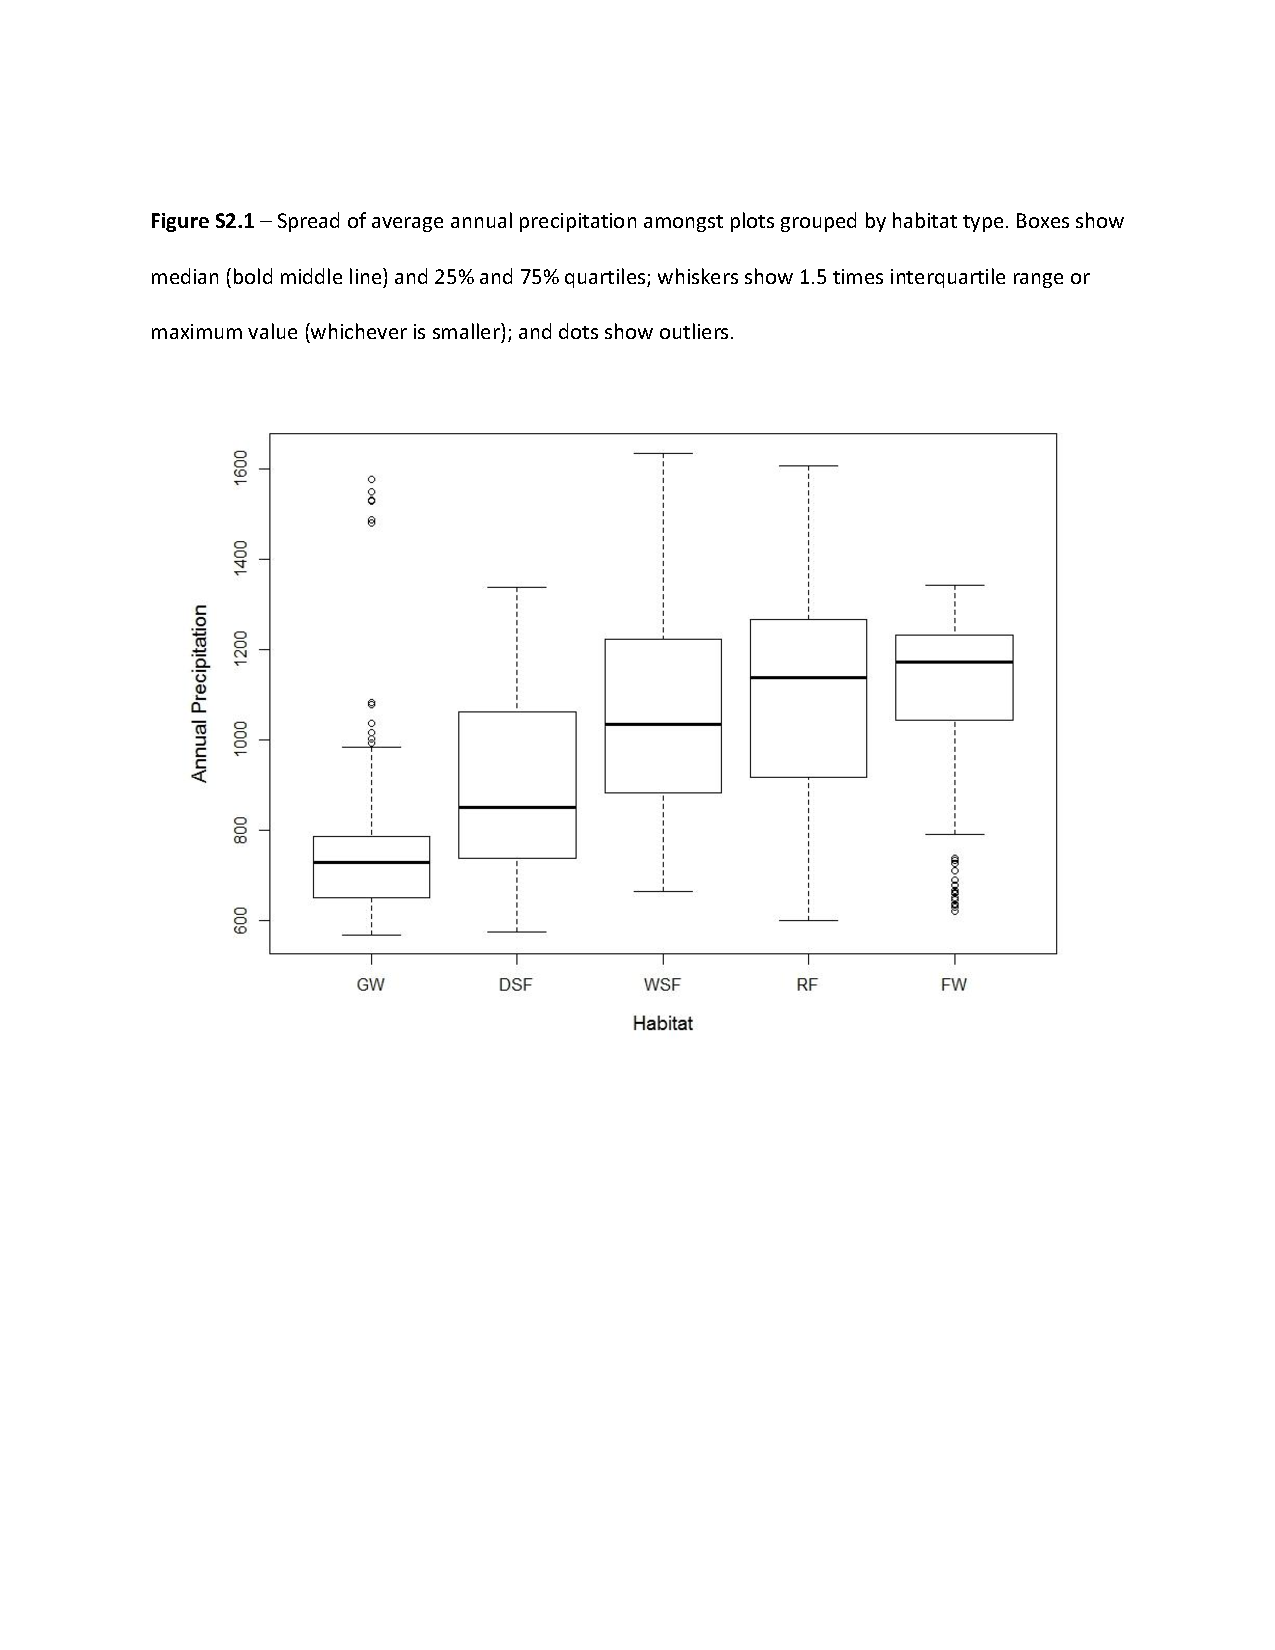
\includepdf[pages={-}, rotateoversize, offset=0.4cm 0cm, addtotoc= {1,section,1,Supplementary figures and tables,hlabel}]{Appendix1/suppmat.pdf}

%!TEX root = ../template.tex
%%%%%%%%%%%%%%%%%%%%%%%%%%%%%%%%%%%%%%%%%%%%%%%%%%%%%%%%%%%%%%%%%%%%
%% appendix2.tex
%% NOVA thesis document file
%%
%% Chapter with example of appendix with a short dummy text
%%%%%%%%%%%%%%%%%%%%%%%%%%%%%%%%%%%%%%%%%%%%%%%%%%%%%%%%%%%%%%%%%%%%
\chapter{Appendix 2 Lorem Ipsum}
\label{app:lorem_ipsum_2}

\lipsum[1-5]

% ******************************* Thesis Appendix B ********************************

\chapter{Supporting information: Chapter 4} 

\graphicspath{{Appendix3/Figs/}}

\section{Phylogeny construction details}

The community phylogeny was constructed using the program phyloGenerator (Pearse and Purvis 2013) and its dependency programs as follows. DNA sequence data for two commonly used plastid gene regions (rbcL and matK) was searched for on GenBank (Benson et al. 2011). Of the 49 taxa in the pool, 30 species were represented, with a further 16 represented by congeneric taxa. Sequences were aligned using MAFFT (Katoh et al. 2005), and the community phylogeny (with divergence times) was estimated under a Bayesian framework using BEAST (Drummond and Rambaut 2007). A constraint tree, generated in Phylomatic (Webb and Donoghue 2005), and dated using the BLADJ algorithm of Phylocom (Webb, Ackerly, and Kembel 2008), was used to place strong priors on the ages and topology of existing highly supported clades. Four independent runs were performed using a GTR model assuming a lognormal relaxed clock with four rate categories, with each run comprising an MCMC chain run for 50,000,000 generations and sampled every 1,000 generations. After checking parameter statistics in TRACER (http://tree.bio.ed.ac.uk/software/tracer/) and removing burnins of 10-20\%, the four independent runs were combined to generate a maximum clade credibility tree. Those taxa represented by congeners were then manually added to the tree, as were the three unrepresented taxa on the basis of their position on the Phylomatic derived constraint tree. 

\newpage

\textbf{Phylogeny for all 49 species in Newick tree format}

\footnotesize((((Gonocarpus micranthus: 32.78964725, Gonocarpus tetragynus: 32.78964725): 124.9441371, ((((Drosera peltata: 19.27769113, Drosera auriculata: 19.27769113): 19.27769113, Drosera pygmaea: 38.55538226): 73.73868839, Drosera spatulata: 112.2940706): 20.52500615, (Stylidium lineare: 112.3064351, (Goodenia stelligera: 74.95393085, Goodenia dimorpha: 74.95393085): 37.35250429): 20.51264166): 24.91470752): 35.6884448, (Burchardia umbellata: 150.2255016, (((((Hypolaena fastigiata: 45.02808262, (((Baloskion gracile: 23.43160533, Eurychorda complanata: 23.43160533): 6.005965644, (Empodisma minus: 12.79282614, Leptocarpus tenax: 12.79282614): 16.64474484): 9.335195904, Lepyrodia scariosa: 38.77276688): 6.25531574): 14.99415044, ((((Plinthanthesis paradoxa: 14.96742327, Aristida warburgii: 14.96742327): 10.6327861, (Themeda australis: 10.795227, Entolasia stricta: 10.795227): 14.80498236): 12.42401627, Tetrarrhena turfosa: 38.02422563): 7.018168824, Austrostipa pubescens: 45.04239445): 14.9798386): 16.64744303, (((Tricostularia pauciflora: 42.6973992, ((Lepidosperma neesii: 11.2529451, Tetraria capillaris: 11.2529451): 18.2730358, (Ptilothrix deusta: 12.26655391, (Schoenus brevifolius: 6.133276955, Schoenus ericetorum: 6.133276955, Schoenus imberbis: 6.133276955, Schoenus lepidosperma: 6.133276955, Schoenus moorei: 6.133276955): 6.133276955): 17.25942698): 13.17141831): 13.29991705, Cyathochaeta diandra: 55.99731626): 10, Xyris gracilis: 65.99731626): 10.67235984): 38.0120084, Haemodorum corymbosum: 114.6816845): 14.17530244, ((Blandfordia nobilis: 105.2018214, (((Thysanotus juncifolius: 31.32190603, (Sowerbaea juncea: 15.35052634, (Lomandra obliqua: 7.67526317, (Lomandra glauca: 4, Lomandra cylindrica: 4): 3.67526317): 7.67526317): 15.97137969): 15.40653782, (Xanthorrhoea resinosa: 31.31985316, (Thelionema umbellatum: 15.65992658, Caesia parviflora: 15.65992658): 15.65992658): 15.40859068): 28.21501178, (Patersonia sericea: 46.94615343, Patersonia fragilis: 46.94615343): 27.9973022): 30.25836574): 9.576595384, (Prasophyllum brevilabre: 106.9427746, Cryptostylis subulata: 106.9427746): 7.835642119): 14.07857018): 21.36851467): 43.1967275): 1.625295448, (Cassytha glabella: 24.29827518, Cassytha pubescens: 24.29827518): 170.7492493);


\normalsize
\subsubsection*{References}

Pearse, W. D. \& Purvis, A. 2013 phyloGenerator: an automated phylogeny generation tool for ecologists. Methods in Ecology and Evolution, 4(7), 692-698.

Drummond, A. J. \& Rambaut, A. 2007 BEAST: Bayesian evolutionary analysis by sampling trees. BMC evolutionary biology, 7(1), 214.

Benson, D. A., Karsch-Mizrachi, I., Lipman, D. J., Ostell, J. \& Sayers, E. W.
GenBank. Nucleic acids research, 39(Database issue), D32-7.

Katoh, K., Kuma, K.-i., Toh, H. \& Miyata, T. 2005 MAFFT version 5: im648
provement in accuracy of multiple sequence alignment. Nucleic acids research,
33(2), 511-8.

Webb, C. O. \& Donoghue, M. 2005 Phylomatic: tree assembly for applied
phylogenetics. Molecular Ecology Notes, 5(1), 181-183.

Webb, C. O., Ackerly, D. D. \& Kembel, S. W. 2008 Phylocom: soft654
ware for the analysis of phylogenetic community structure and trait evolution. Bioinformatics (Oxford, England), 24(18), 2098-100.

\section{Equations for calculating \textit{D}$_{nn}$ and \textit{D}$_{pw}$}

Phylogenetic and functional nearest-neighbour dissimilarity (\textit{D}$_{nn}$, the beta diversity analogue of MNTD) is given by:

$$D_{nn} = f_{A}\sum_{i=1}^{S_{A}}f_{i} min \delta _{ib} + f_{B}\sum_{j=1}^{S_{B}}f_{j}min \delta _{jb}$$

where \textit{SA} is the number of species in the community at time A, \textit{SB} is the number of species in the community at time B, $\mathrm{min \delta _{\mathit{ib}}}$ is the phylogenetic or functional distance of species \textit{i} at time B to its nearest neighbour at time A, $\mathrm{min \delta _{\mathit{ja}}}$ is the phylogenetic or functional distance of species \textit{j} at time B to its nearest neighbour at time A, $\mathit{f_{i}}$  is the relative abundance of species \textit{i} in the community at time A, and finally $\mathit{f_{j}}$ is the relative abundance of species \textit{j} in the community at time B. 

Similarly, pairwise dissimilarity (\textit{D}$_{pw}$, the beta diversity analogue of MPD) is given by:

$$D_{pw} = f_{A}\sum_{i=1}^{S_{A}}f_{i}\overline{\delta _{ib}} + f_{B}\sum_{j=1}^{S_{B}}f_{j}\overline{\delta _{ja}}$$

where terms shared with \textit{D}$_{nn}$ are equivalent, and $\overline{\delta _{ib}}$ is the mean pairwise phylogenetic or functional distance between species i in the community at time A and all species in the community at time B, and $\overline{\delta _{jb}}$ is the mean pairwise phylogenetic of functional distance between species j in the community at time B and all species in the community at time A. Note that as for MNTD and MPD, phylogenetic distance was first square-root transformed before input into both \textit{D}$_{nn}$ and \textit{D}$_{pw}$.

\subsubsection*{References}

Ricotta, C. \& Burrascano, S. 2009 Testing for differences in beta diversity
with asymmetric dissimilarities. Ecological Indicators, 9(4), 719-724.

Swenson, N. G., Stegen, J. C., Davies, S. J., Erickson, D. L., Forero-Monta~na,
J., Hurlbert, A. H., Kress, W. J., Thompson, J., Uriarte, M. et al. 2012
Temporal turnover in the composition of tropical tree communities: functional
determinism and phylogenetic stochasticity. Ecology, 93(3), 490-499.

\section{Phylogenetic signal in traits}


\footnotesize Table S4.1. Phylogenetic signal in functional traits quantified using either Blomberg's \textit{K} statistic for continuously defined traits or the `Fixed Tree, Character Randomly Reshuffled' model of Maddison \& Slatkin (1991) for traits coded ordinally.
\begin{table}[H]
\centering
\begin{tabular}{lcc}
\hline Trait & \textit{K} statistic & p-value\\
\hline log$_{10}$(seed weight)
 & 0.385 & 0.001 \\ 
log$_{10}$(maximum height)
 & 0.647 & 0.001 \\ 
Fire response & - & $<$ 0.001 \\ 
Raunki\ae r life-form
 & - & 0.005 \\ 
Fecundity & - & 0.003 \\ 
Longevity
 & - & $<$ 0.001 \\ 
Seedbank persistence
 & - & $<$ 0.001 \\ 
\hline 
\end{tabular} 
\end{table}

\pagebreak

\section{Temporal change in phylogenetic and functional community structure: supplementary figures}
\sectionmark{Temporal change in community structure: supp. figs.}

The following figures, which correspond with Figure 2 in the main article, show phylogenetic and functional community structure through time when the species pool is constrained to only include monocots or only Polaes. Trendlines correspond to models of MNTD/MPD/F-MNTD/F-MPD vs. time for all plots/sites through the first four years of sampling (solid line); plots/sites that only burnt in 1994 (dashed line) and plots that burnt in 1994 and 2001 (dotted lines). Trend lines shaded black indicate significant slope coefficients at p $<$ 0.05; grey lines indicate insignificant slopes.

\begin{figure}[H]
\centering
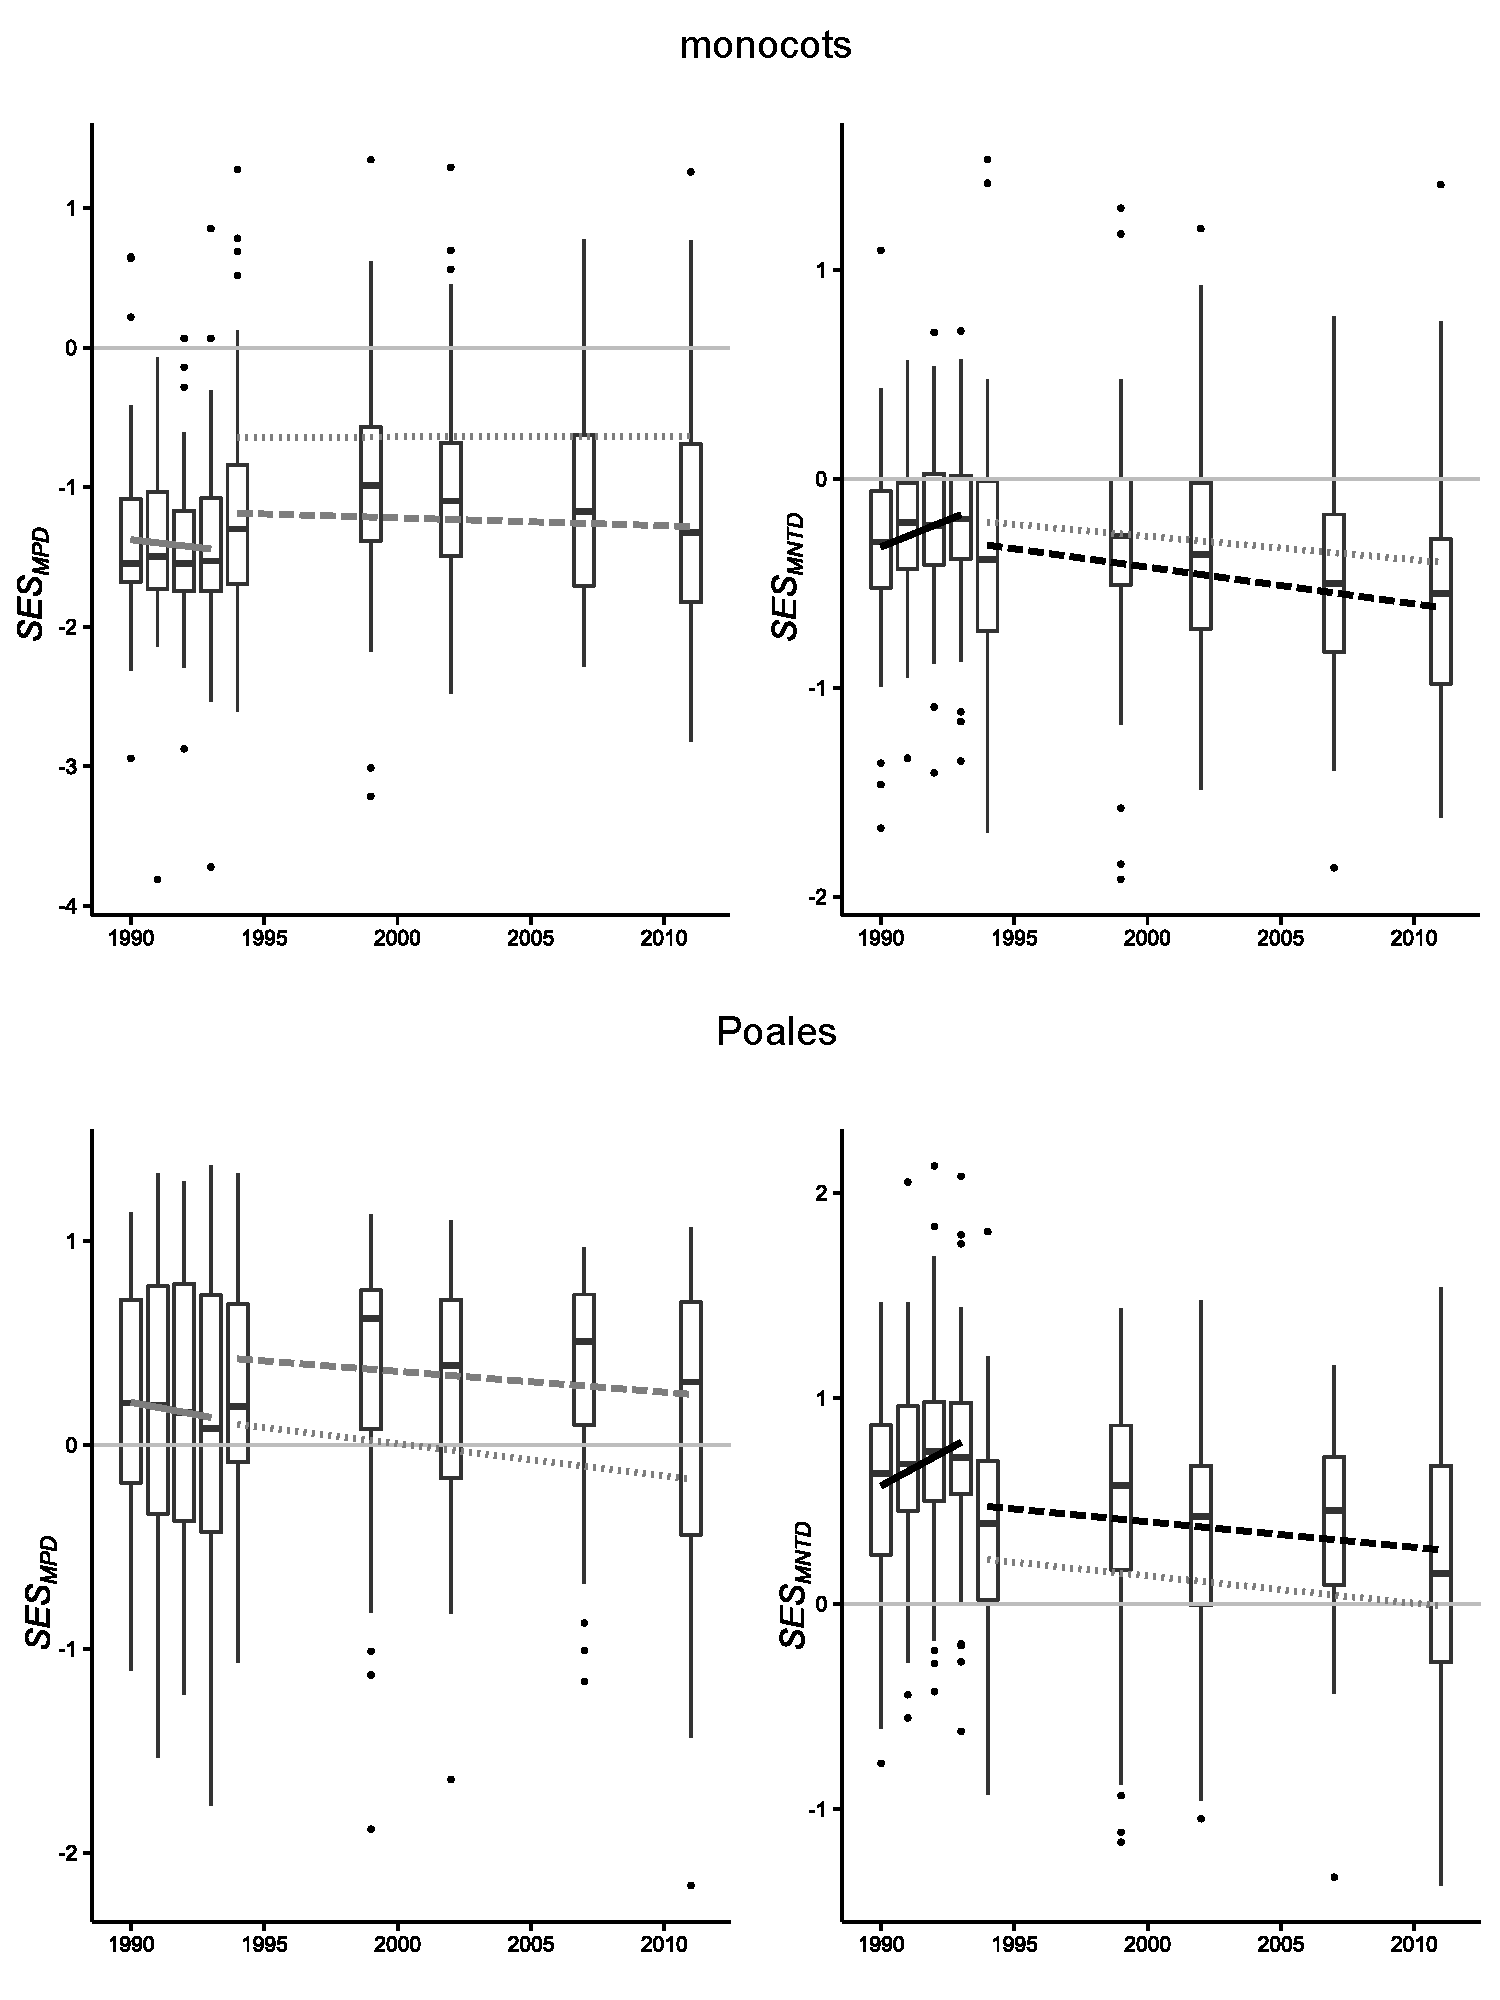
\includegraphics[width=0.7\linewidth]{phy_poales_mono_alphadiv}\\
\footnotesize Figure S4.1. Phylogenetic community structure of monocots and Poales through time at the plot scale.
\end{figure}

\begin{figure}[H]
\centering
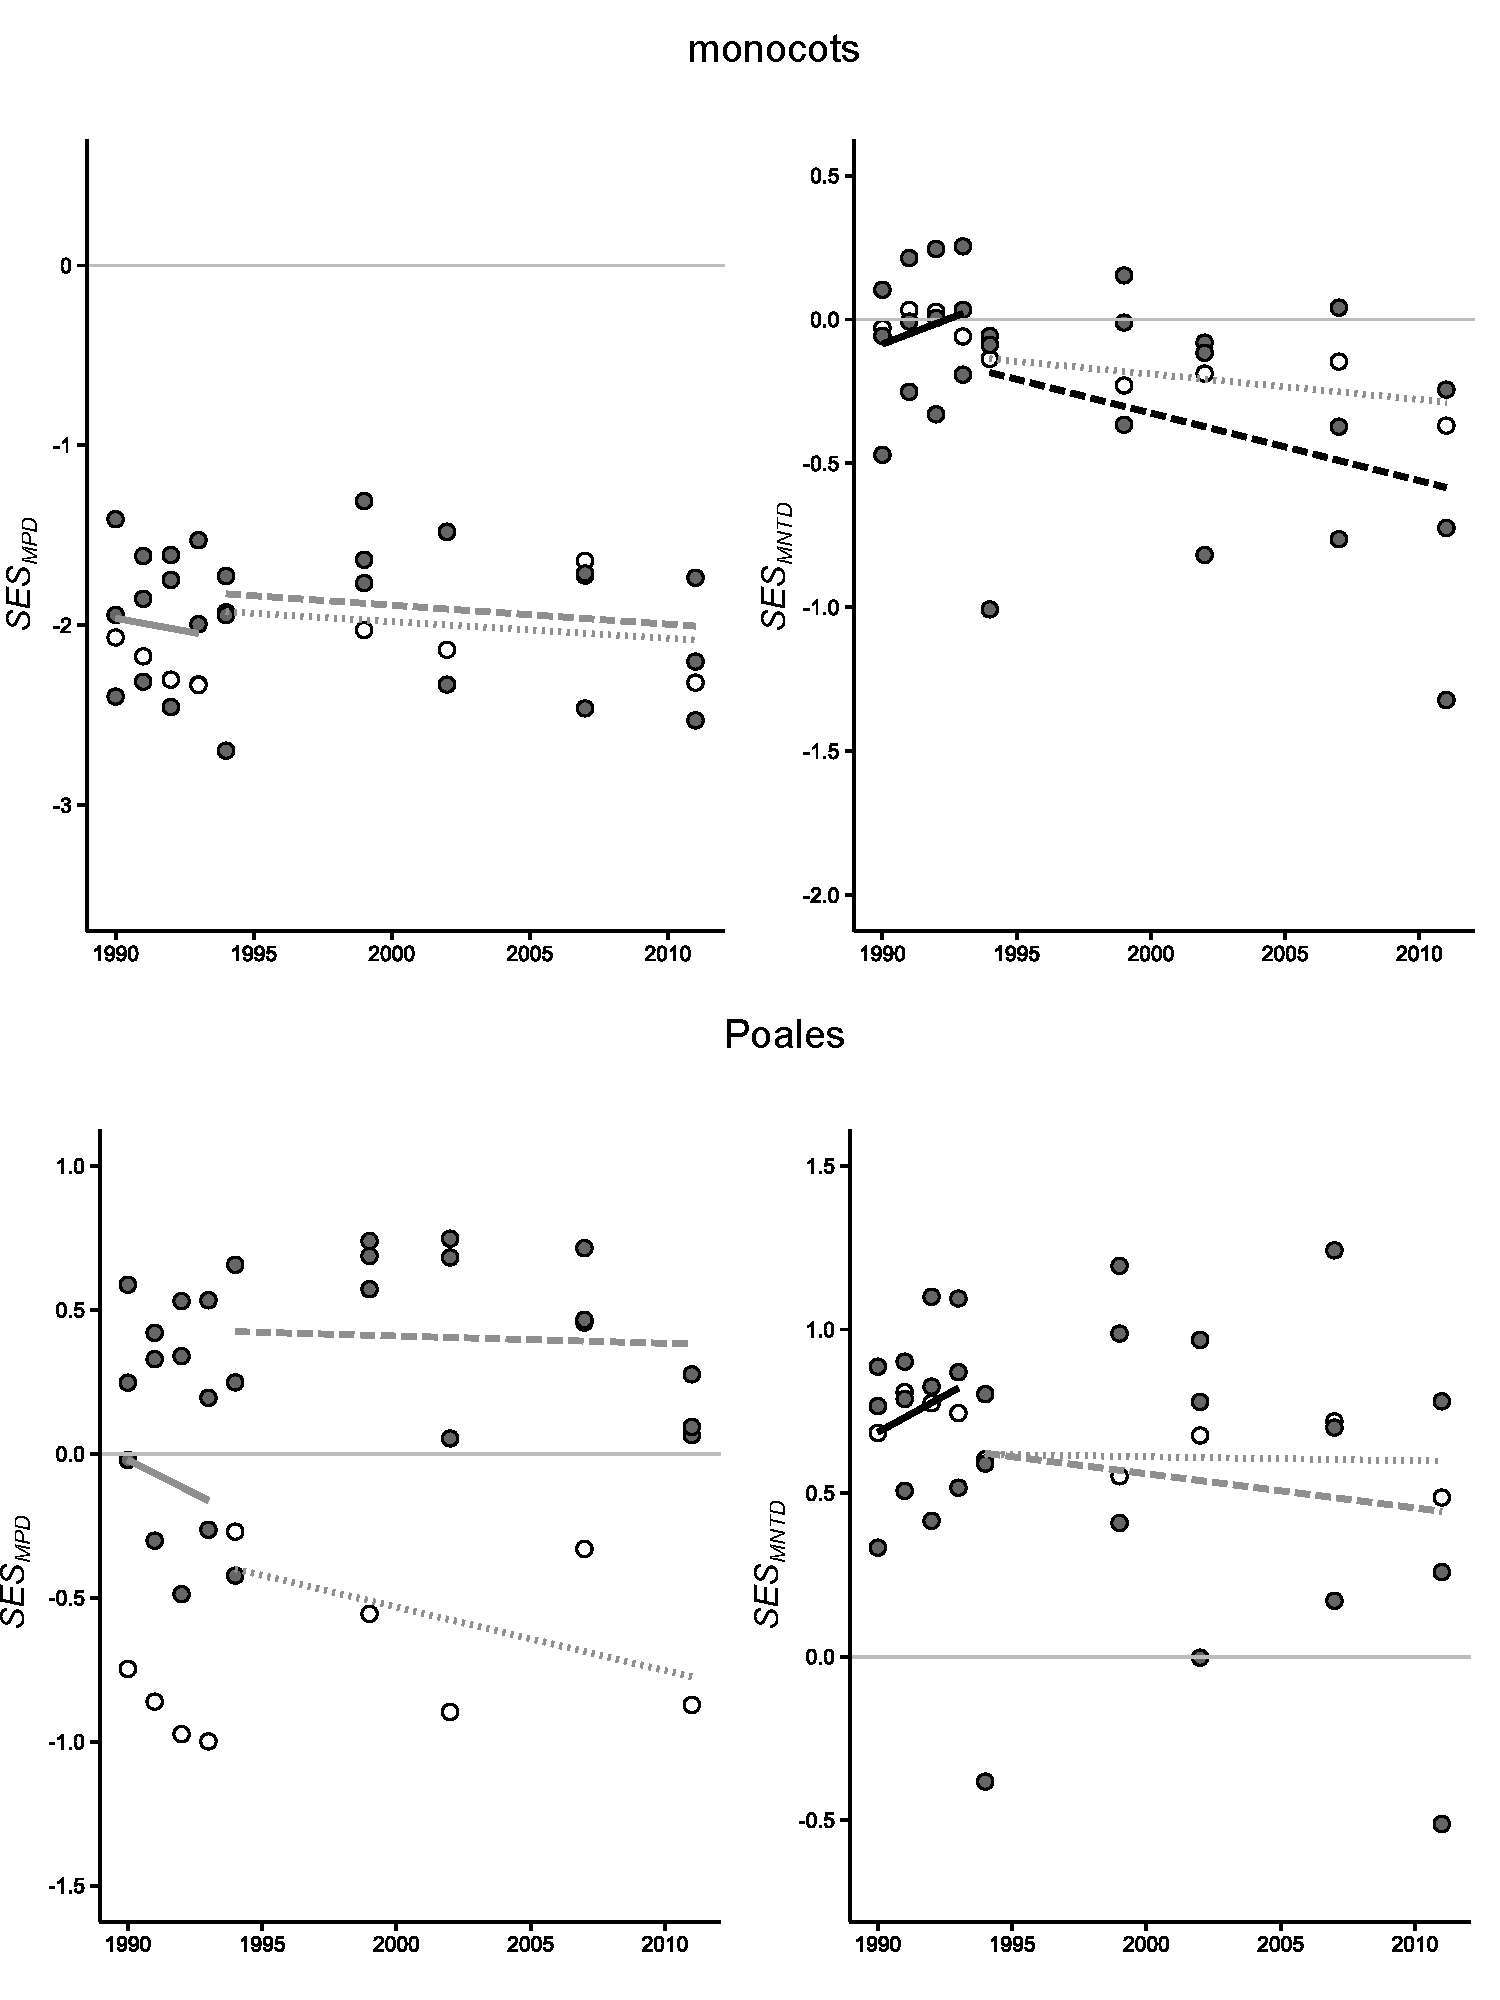
\includegraphics[width=0.7\linewidth]{phy_poales_mono_alphadiv_transectscale_points}\\
\footnotesize Figure S4.2. Phylogenetic community structure of monocots and Poales through time at the site scale.
\end{figure}

\begin{figure}[H]
\centering
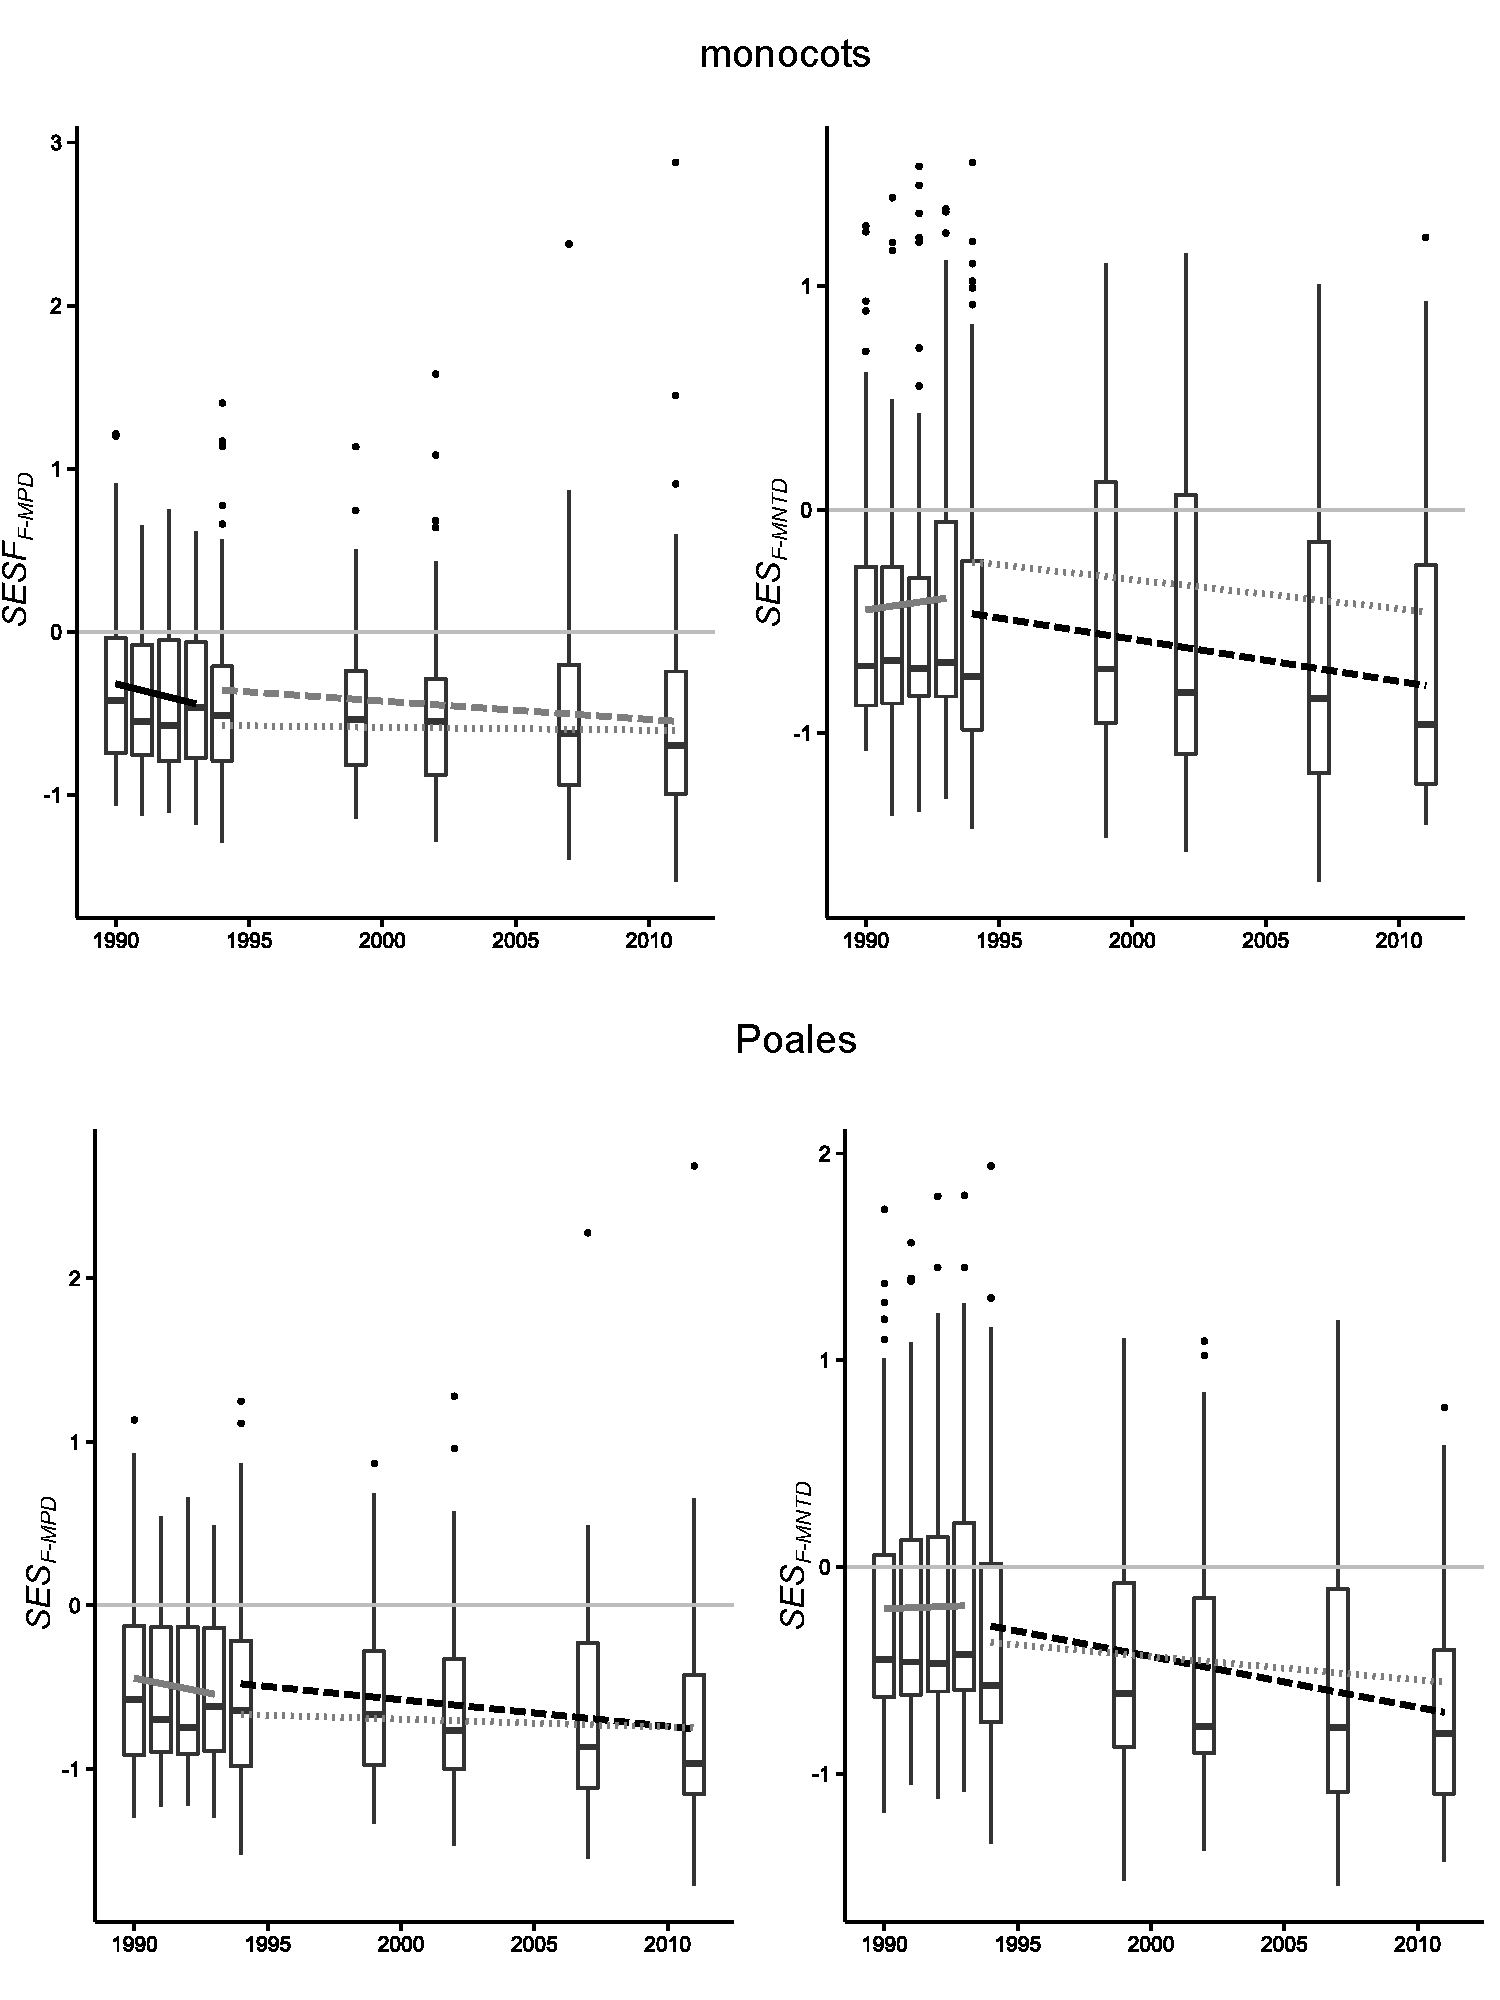
\includegraphics[width=0.7\linewidth]{func_poales_mono_alphadiv}\\
\footnotesize Figure S4.3. Functional community structure of monocots and Poales through time at the plot scale.
\end{figure}

\begin{figure}[H]
\centering
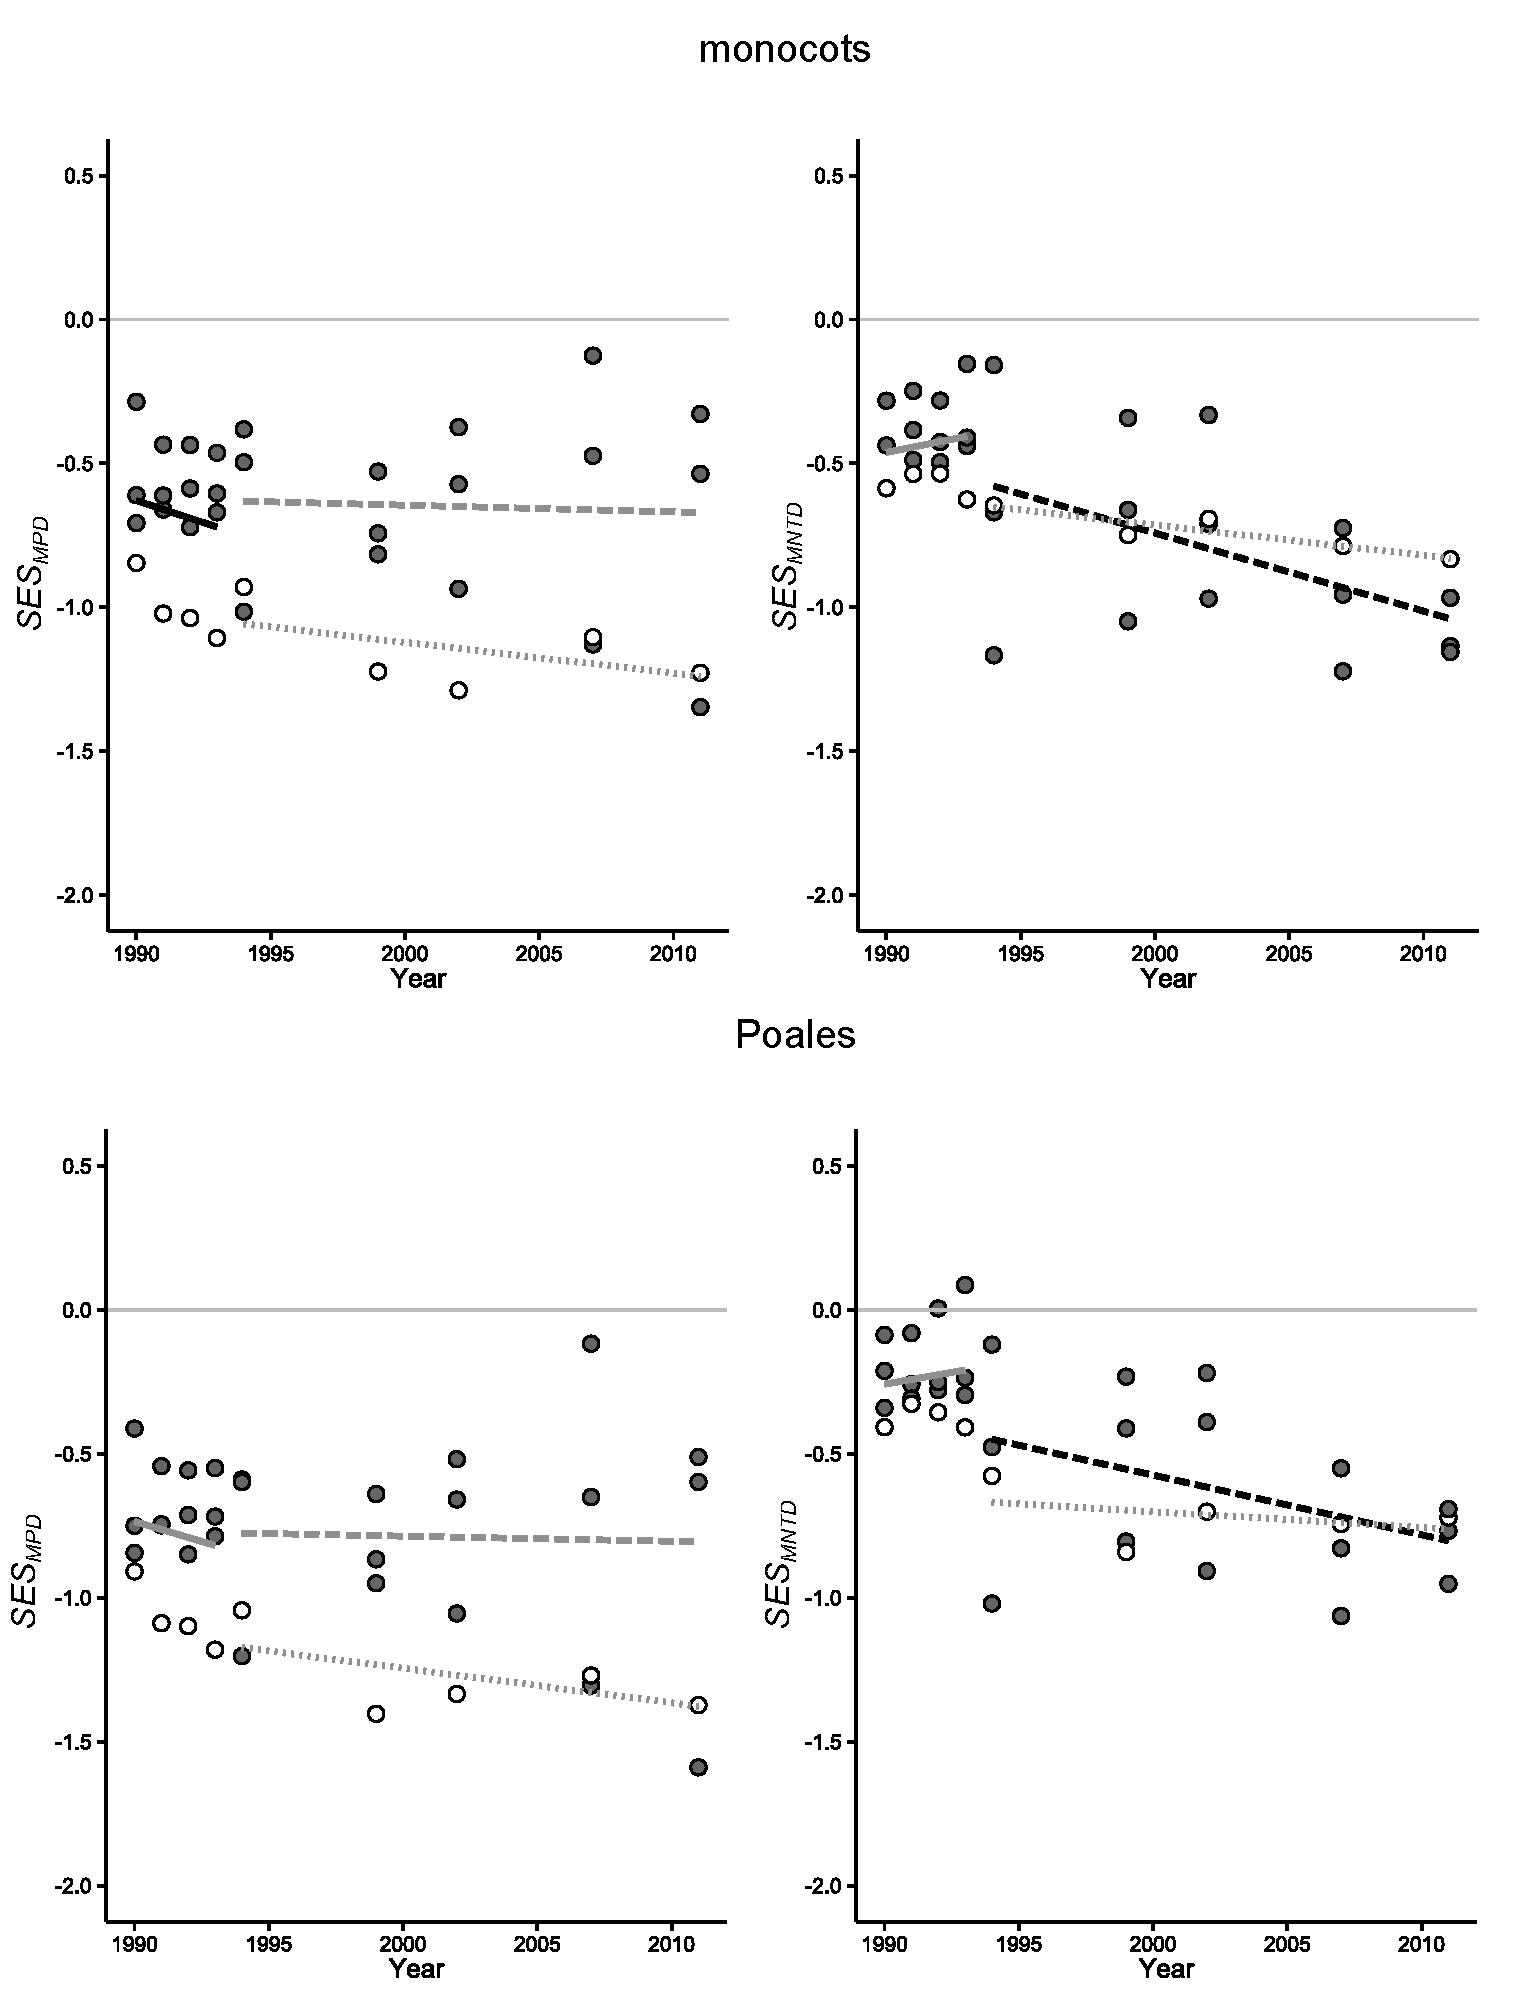
\includegraphics[width=0.7\linewidth]{func_alphadiv_poales_mono_scatter_transectscale}\\
\footnotesize Figure S4.4. Functional community structure of monocots and Poales through time at the site scale.
\end{figure}

\clearpage

\section{Temporal phylogenetic and functional beta turnover: supp. figs.}
\sectionmark{Temporal beta turnover: supp. figs.}

\begin{figure}[H]
\centering
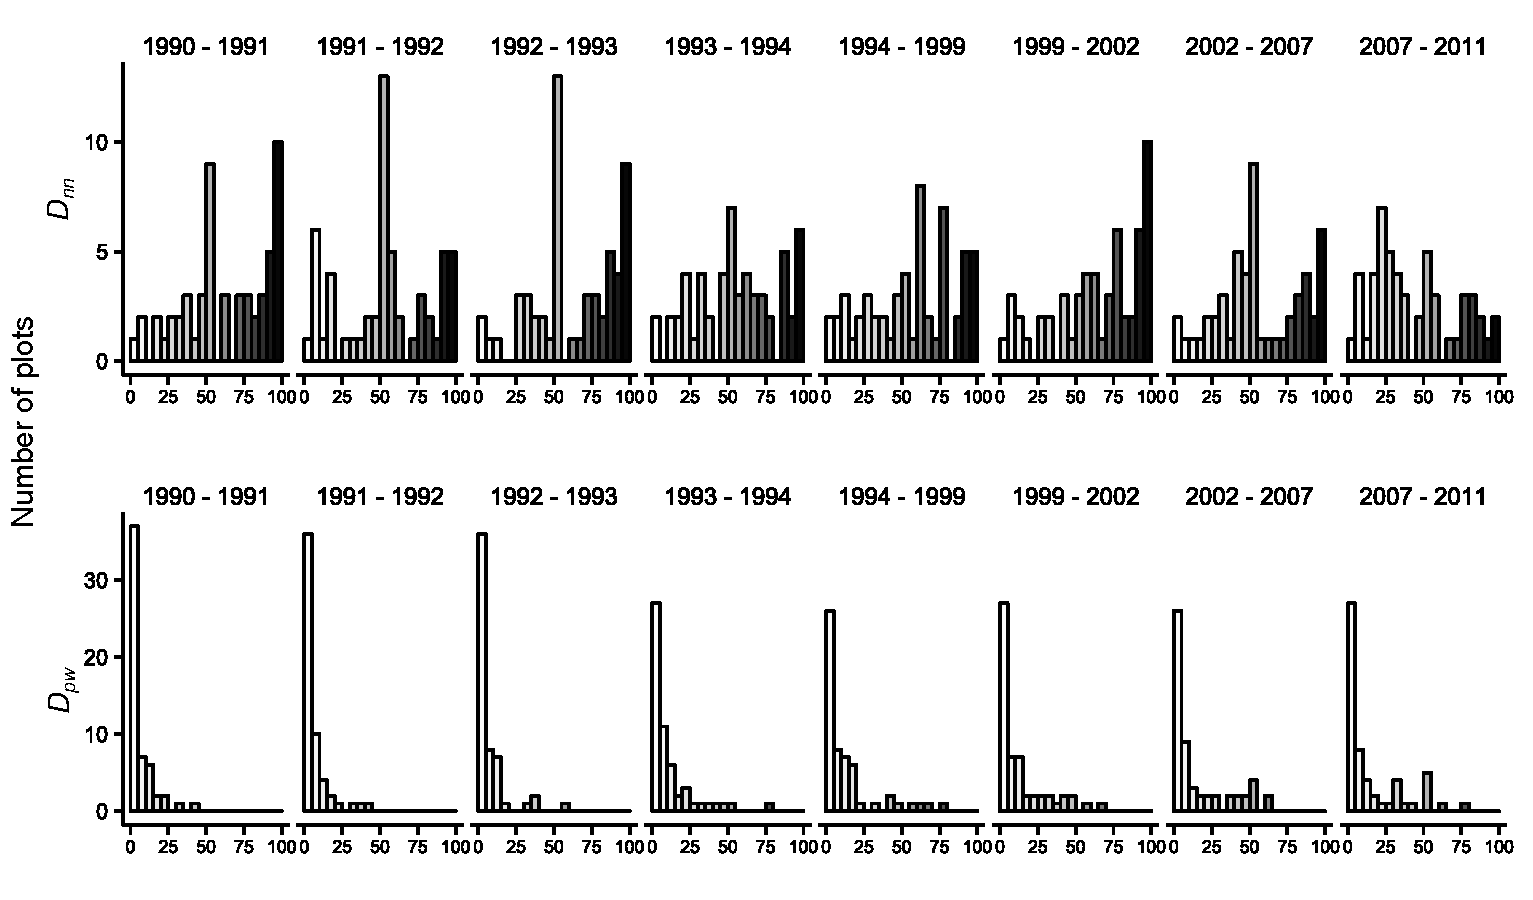
\includegraphics[width=1.0\linewidth]{full_phybeta_int}\\
\footnotesize Figure S4.5. Temporal phylogenetic beta turnover quantified by \textit{D}$_{nn}$ and  \textit{D}$_{pw}$ relative to the immediately preceding census point. Low quantile scores (white) indicate low turnover in phylogenetic composition relative to the observed rate of taxonomic turnover; high quantile scores (black) indicate high turnover in phylogenetic composition relative to the observed rate of taxonomic turnover. Values $<$2.5 or $>$97.5 are significant at the 0.05 level.
\end{figure}

\begin{figure}[H]
\centering
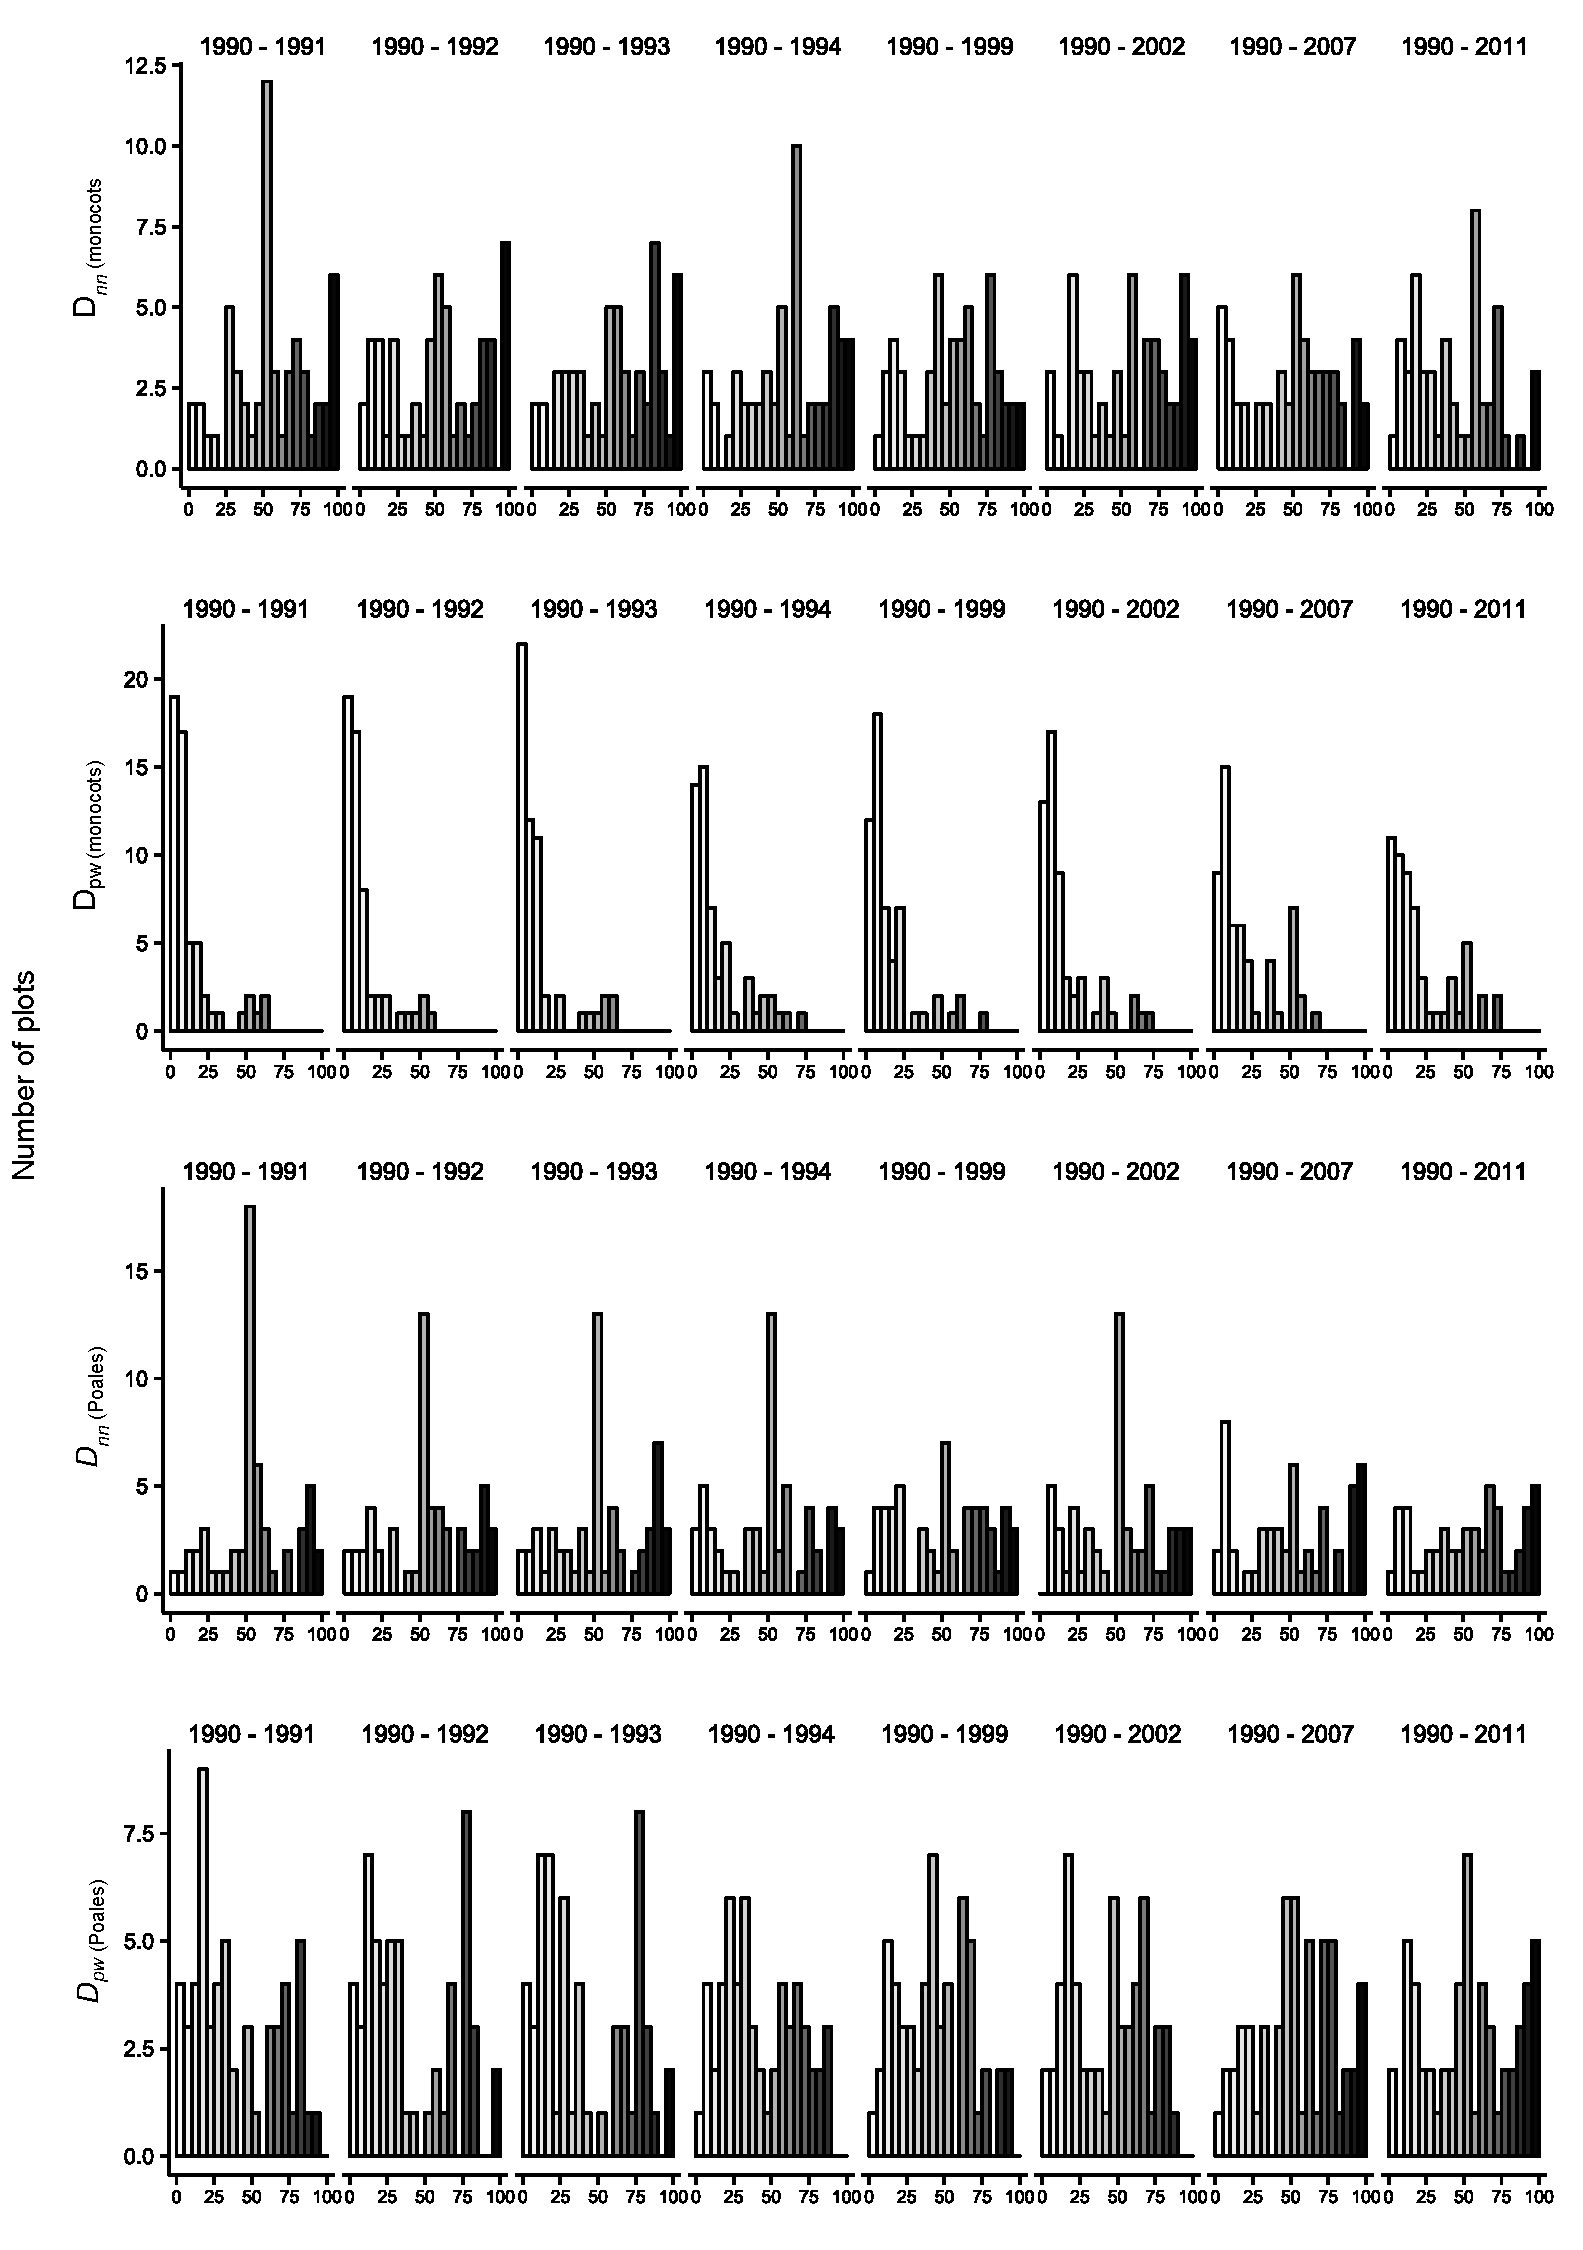
\includegraphics[width=0.8\linewidth]{mono_poales_phybeta}\\
\footnotesize Figure S4.6. Temporal phylogenetic beta turnover (monocots and Poales) quantified by \textit{D}$_{nn}$ and \textit{D}$_{pw}$ relative to the first census point. Low quantile scores (white) indicate low turnover in phylogenetic composition relative to the observed rate of taxonomic turnover; high quantile scores (black) indicate high turnover in phylogenetic composition relative to the observed rate of taxonomic turnover. Values $<$2.5 or $>$97.5 are significant at the 0.05 level.
\end{figure}


\begin{figure}[H]
\centering
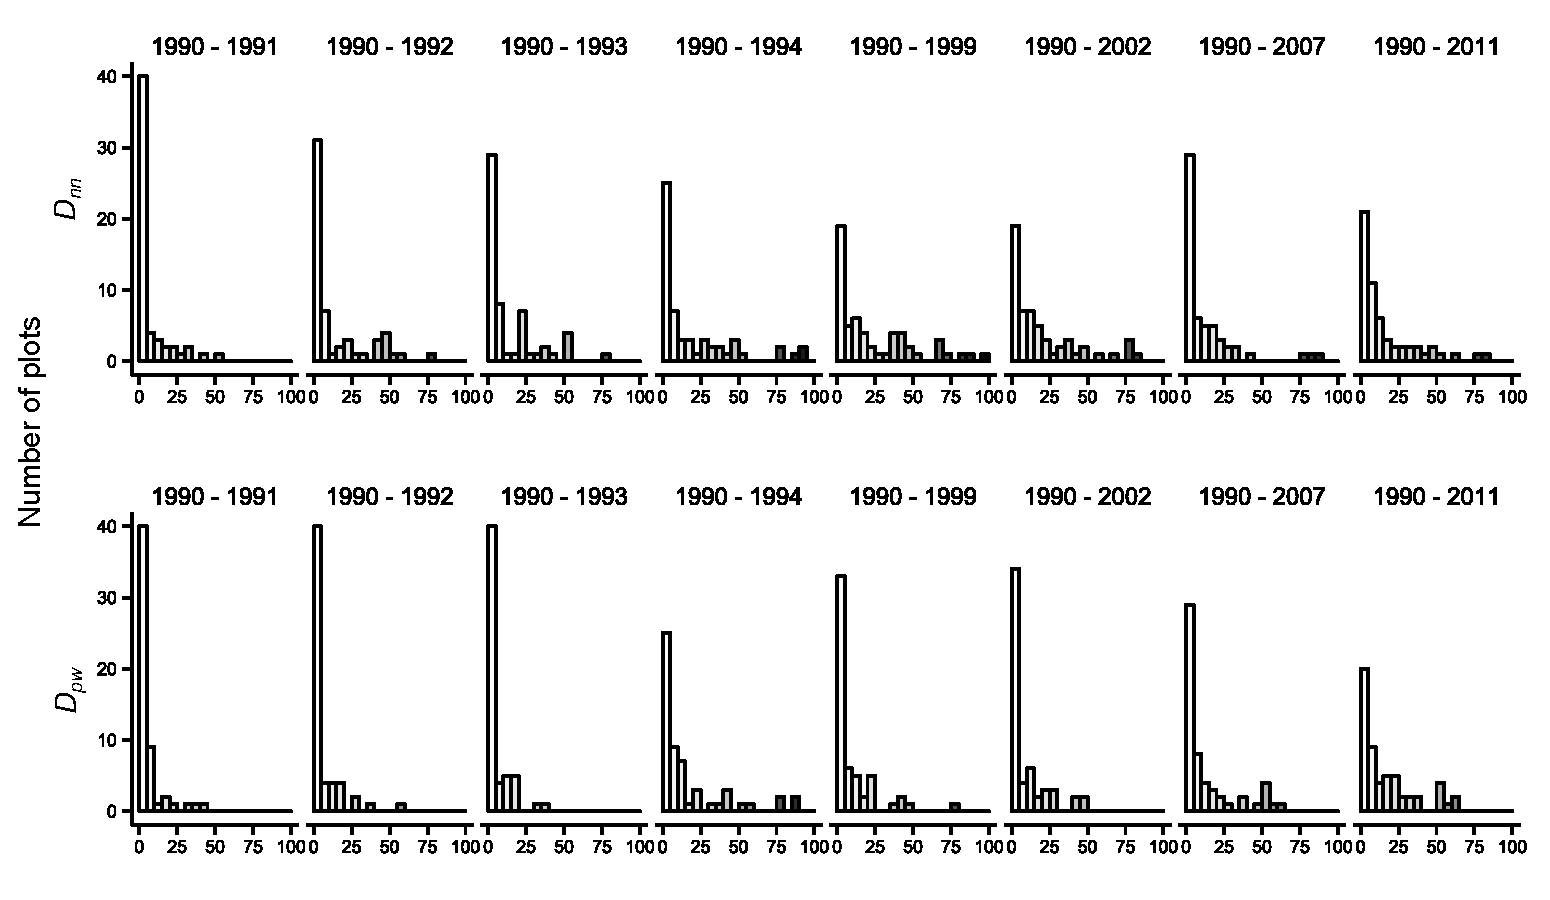
\includegraphics[width=1.0\linewidth]{full_funcbeta}\\
\footnotesize Figure S4.7. Temporal functional beta turnover quantified by \textit{D}$_{nn}$ and  \textit{D}$_{pw}$ relative to the first census point. Low quantile scores (white) indicate low turnover in phylogenetic composition relative to the observed rate of taxonomic turnover; high quantile scores (black) indicate high turnover in phylogenetic composition relative to the observed rate of taxonomic turnover. Values $<$2.5 or $>$97.5 are significant at the 0.05 level.
\end{figure}



\begin{figure}[H]
\centering
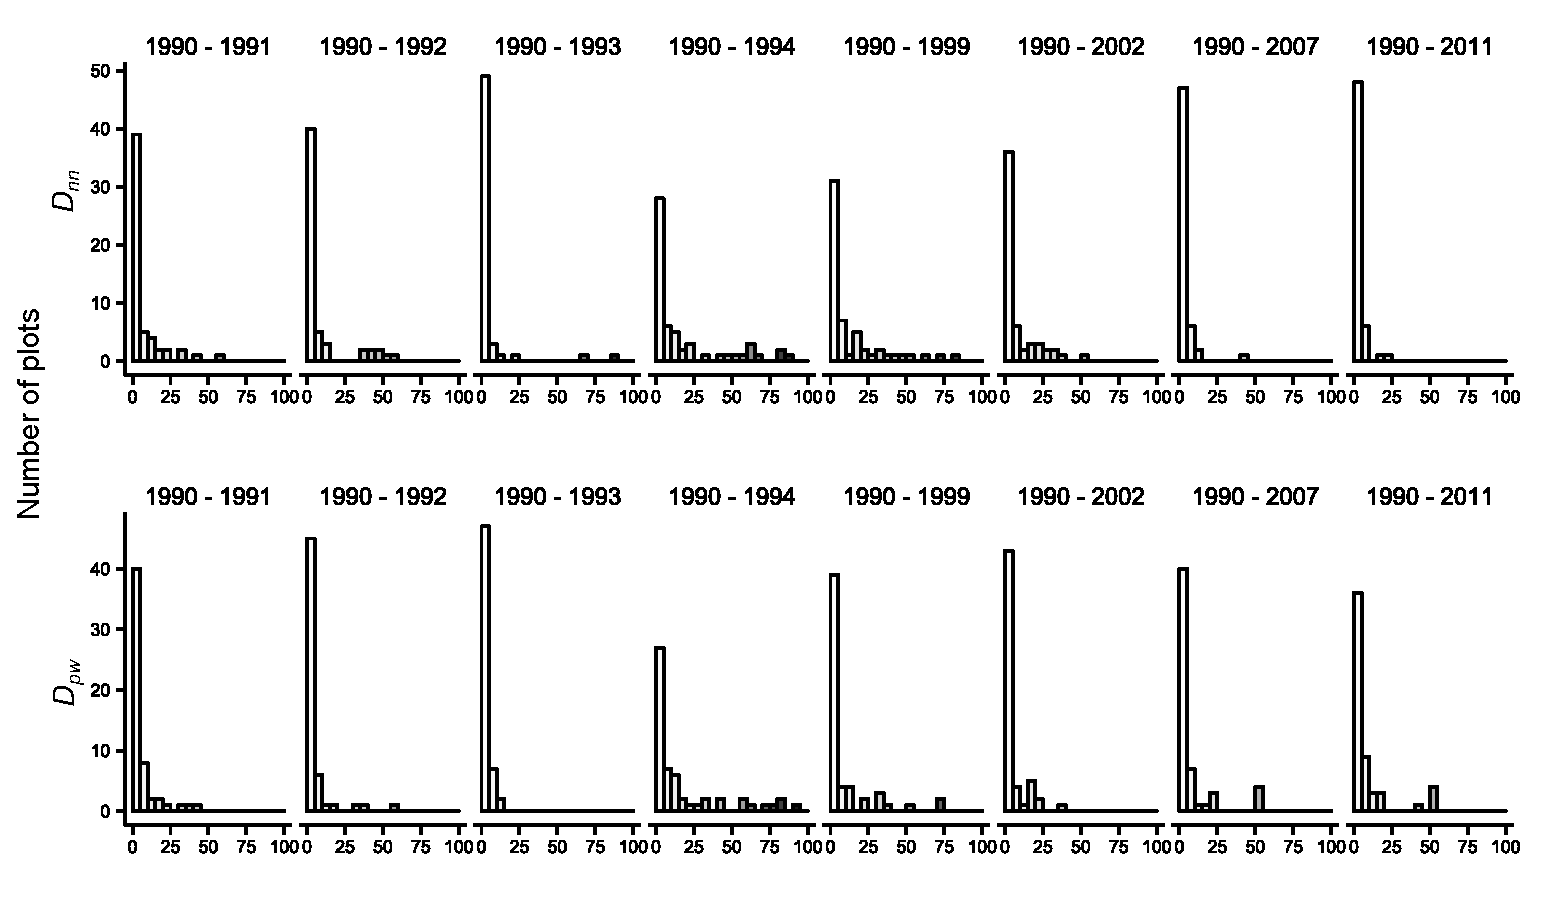
\includegraphics[width=1.0\linewidth]{full_funcbeta_int}\\
\footnotesize Figure S4.8. Temporal functional beta turnover quantified by \textit{D}$_{nn}$ and  \textit{D}$_{pw}$ relative to the immediately preceding census point. Low quantile scores (white) indicate low turnover in phylogenetic composition relative to the observed rate of taxonomic turnover; high quantile scores (black) indicate high turnover in phylogenetic composition relative to the observed rate of taxonomic turnover. Values $<$2.5 or $>$97.5 are significant at the 0.05 level.
\end{figure}

\begin{figure}[H]
\centering
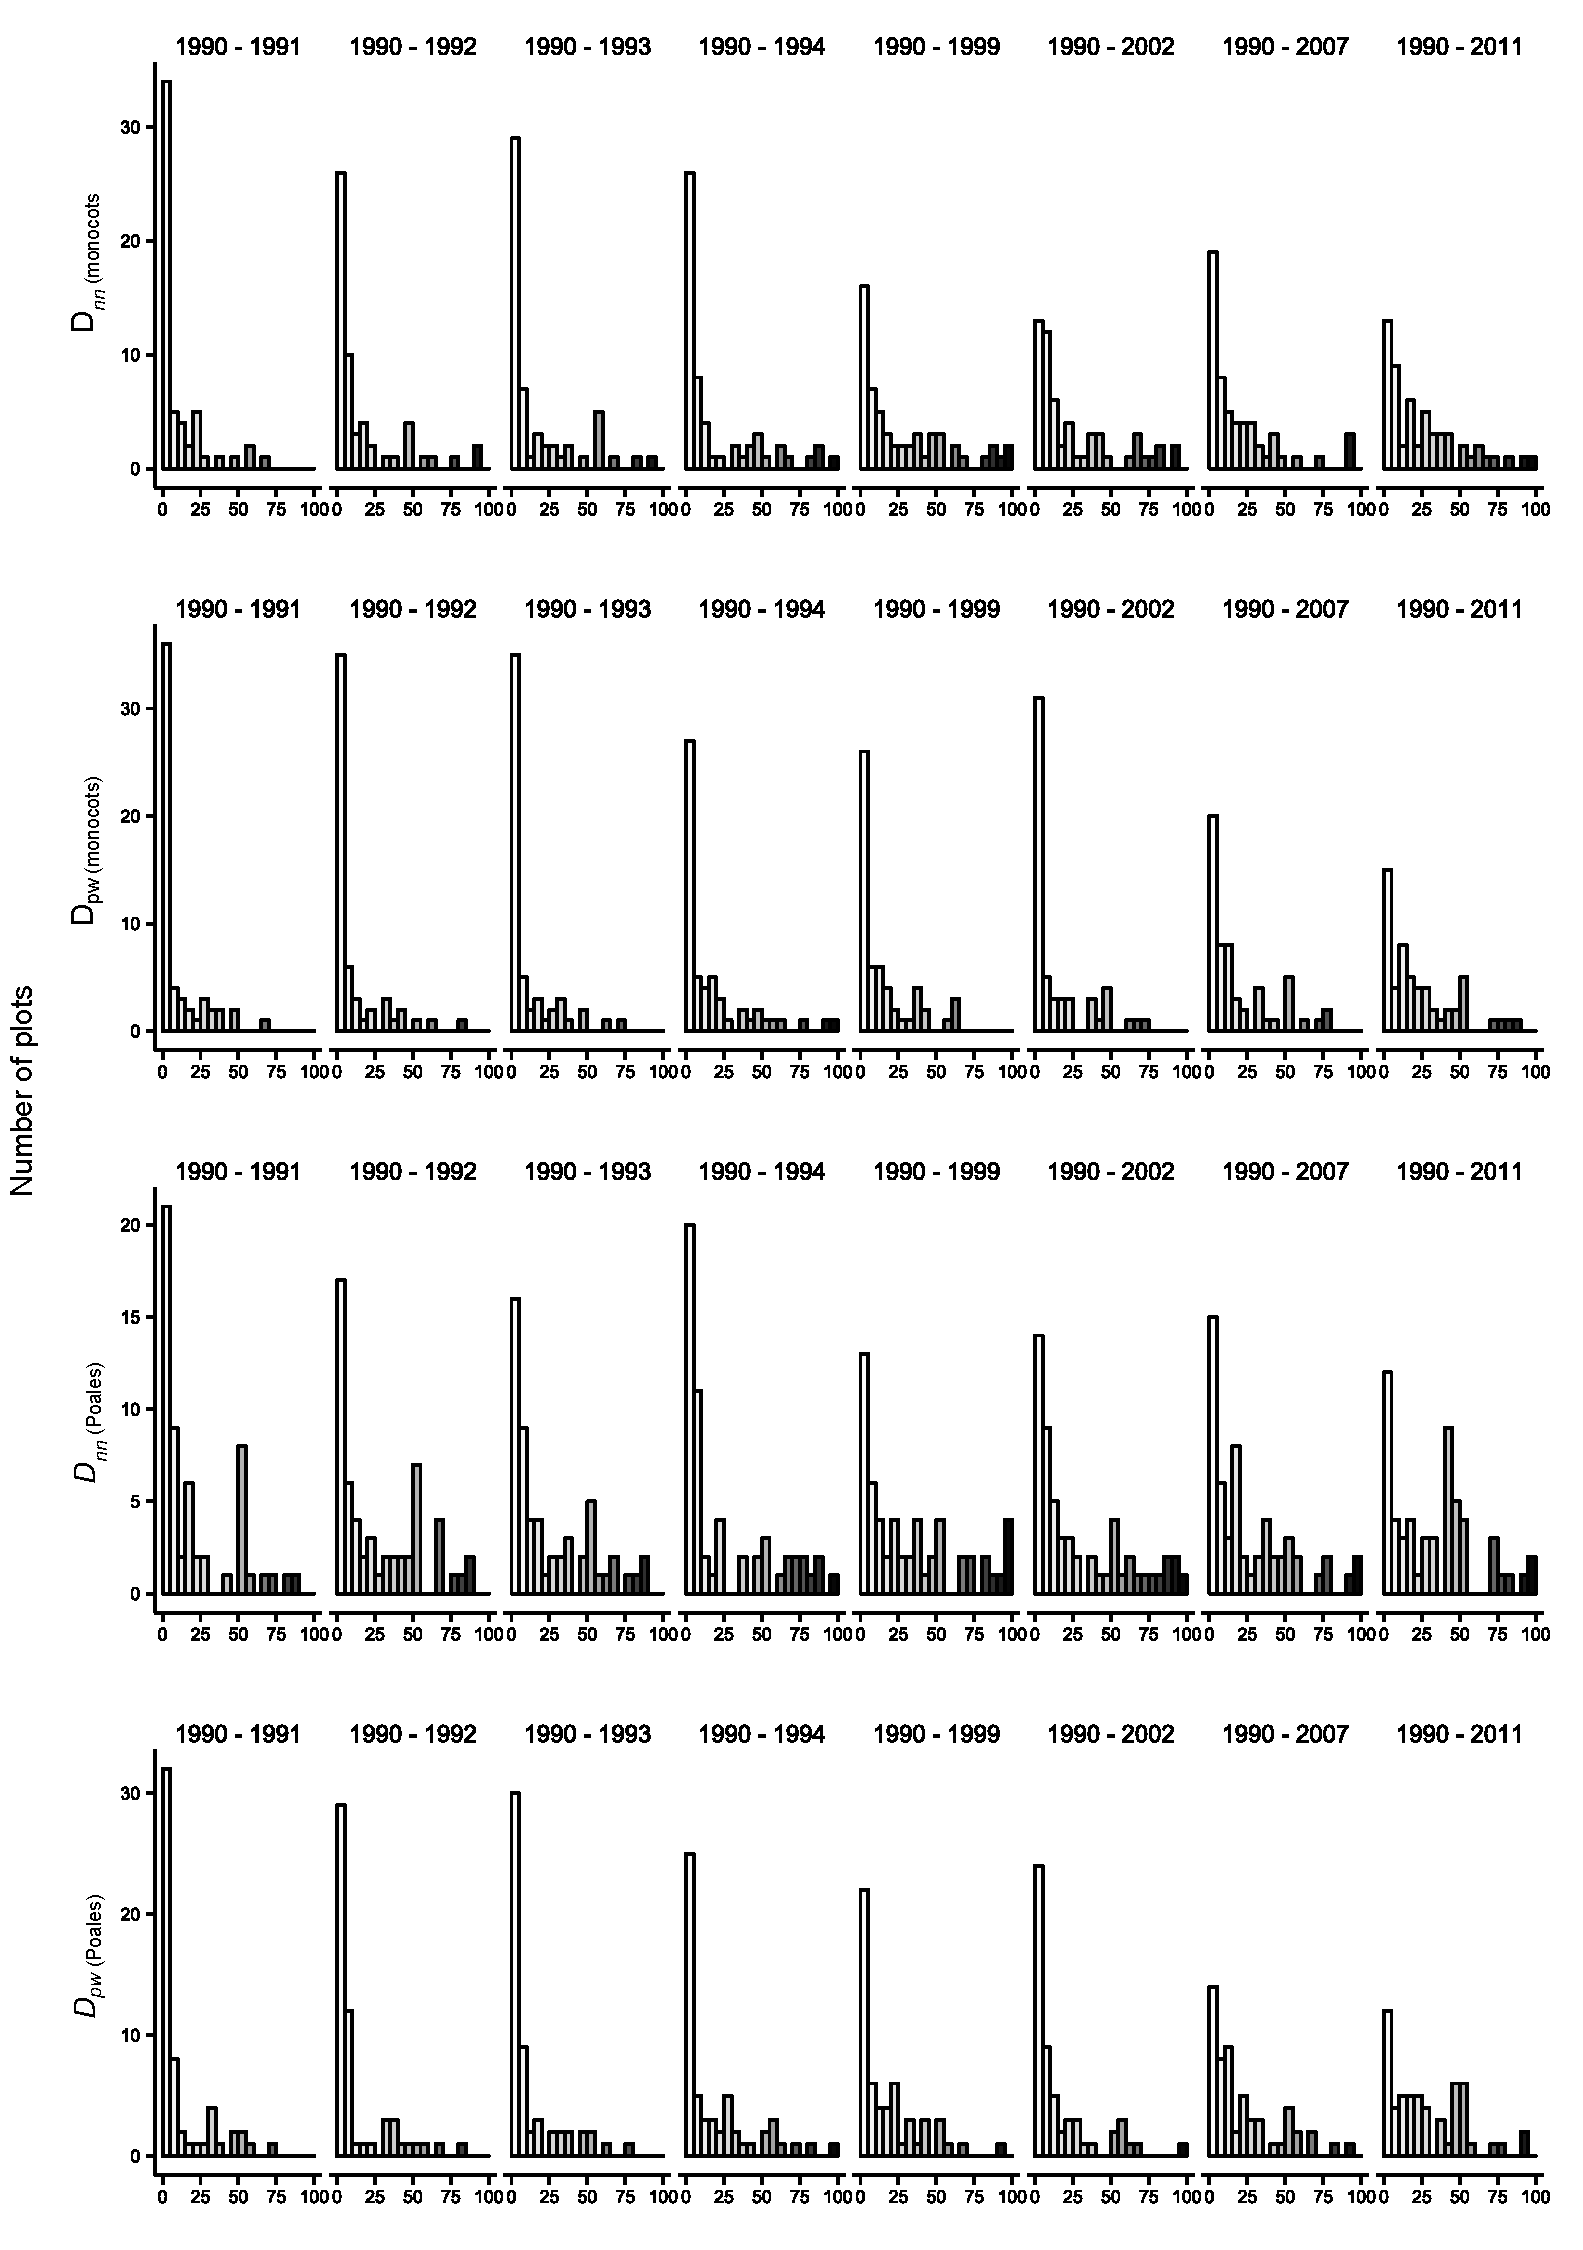
\includegraphics[width=0.8\linewidth]{mono_poales_funcbeta}\\
\footnotesize Figure S4.9. Temporal functional beta turnover (monocots and Poales) quantified by \textit{D}$_{nn}$ and \textit{D}$_{pw}$ relative to the first census point. Low quantile scores (white) indicate low turnover in phylogenetic composition relative to the observed rate of taxonomic turnover; high quantile scores (black) indicate high turnover in phylogenetic composition relative to the observed rate of taxonomic turnover. Values $<$2.5 or $>$97.5 are significant at the 0.05 level.
\end{figure}

\section{Species accumulation curve}

\begin{figure}[H]
\centering
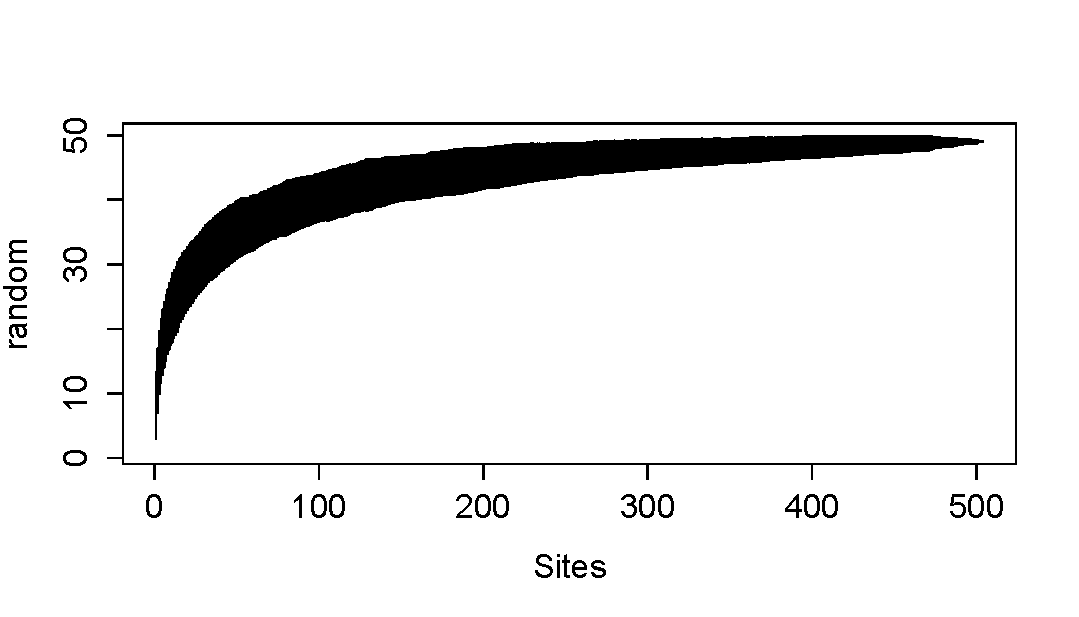
\includegraphics[width=1.0\linewidth]{sppaccum-sites}\\
\footnotesize Figure S4.10. Species accumulation curve obtained from 100 permutations of site in random order. Width denotes standard error.
\end{figure}




% bibliography.tex should include either 
% \bibliographystyle{...}
% \bibliography{mythesis}
% or some other way of doing the bibliography
\printbibliography

\end{document}

